\documentclass[ngerman,twoside, a4paper,12pt]{scrreprt}
\usepackage[T1]{fontenc}
\usepackage[latin1]{inputenc}
\usepackage{psfrag}		 % Um Formeln in Bilder zu schreiben
%\usepackage{graphfig}
\usepackage{makeidx}
\usepackage{amsmath}
\usepackage{textcomp}
\usepackage{pifont}
\usepackage{floatflt}
%\usepackage{pst-pdf}
%\usepackage{pst-all}
%\usepackage{pst-add}
%\usepackage{picins}
\usepackage{makebox}
\usepackage{fancybox}
\usepackage{listings}   %n�tig zum Einbinden von Listings (Quellcode)
\usepackage{vmargin}  %Bestimmt die Seitengeometrie
%\setmargins{2.5cm}{1.5cm}{16.2cm}{22.5cm}%
\setmarginsrb{2.5cm}{1.5cm}{2.5cm}{1.5cm}%
							{7mm}{1.2cm}{4mm}{1.5cm}
% Setzen der geometrischen Gr��en: {links}{oben}{rechts}{unten}%
%																	 {kopfh�he}{kopfabstand}{fu�h�he}{fu�abstand}
\setkomafont{sectioning}{\normalfont \bfseries}
\usepackage{fancyhdr}


\usepackage{hyperref}
\usepackage{booktabs}

\hypersetup{
	pdftitle={Skript ADS-Praktikum},
	pdfauthor={\textcopyright\ LTE Andreas Schedel \& Daniel Glaser},
	bookmarksopen=true,
	bookmarksopenlevel=1
}

\usepackage[svgnames, table, hyperref]{xcolor}
\usepackage{marvosym}
\usepackage{graphicx}

\usepackage[ngerman]{babel}
% Legt fest, wie viele Ebenen tief die Nummerierung bei Aufz�hlungen sind
\setcounter{secnumdepth}{3}

\usepackage{multido}

\usepackage{shorttoc}

\usepackage{ifthen}

% Are we producing colored output
\newcommand{\printcolor}{\boolean{true}}

% true --> Musterl�sung, false --> Studentenskript
% Are we as perfect that we know the solution ;-)
\newcommand{\printsolution}{\boolean{true}}

% Do we use XEmacs or the integrated something
\newcommand{\xemacs}{\boolean{false}}

% Include notes for developing the script
\newcommand{\shownotes}{\boolean{false}}

% The relative path to the VHDL Source while tex-compiling
\newcommand{\texpathtovhdl}[1]{../ispLEVER/}

% This command is useful for changing the root of the students
\newcommand{\pathtoadsp}[1]{\begin{quote}\texttt{P:\textbackslash #1}\end{quote}}
\newcommand{\pathtoisp}[1]{\pathtoadsp{ispLEVER\textbackslash #1}}
\newcommand{\pathtomatlab}[1]{\begin{quote}\texttt{MATLAB\_src\textbackslash #1}\end{quote}}

% The question and answer game
% Arg 1: Count of lines to be insertet
% Arg 2: The answer to the question
\newcommand{\answergame}[2]{%
  \paragraph{}
	\begin{samepage}
		\ifthenelse{\printsolution}
		{
			\fbox
			{
				\begin{minipage}{0.85\linewidth}
					#2
				\end{minipage}
			}
		}
		{
			%else
			\begin{minipage}{0.94\linewidth}
				%\textbf{L�sung:}\\
				\multido{\i=0+1}{#1}{
					\begin{minipage}{\linewidth}
						\hrulefill
					\end{minipage}
				}
			\end{minipage}
		}
	\end{samepage}
}

\newcommand{\answerfig}[3]{%
	\ifthenelse{\printsolution}{	
		\begin{center}
			\includegraphics{#3}
			\vspace{#2}
		\end{center}
	}{%
		\vspace{#1}
	}
}
% Something for design
\newcommand{\graphbox}[2]{%
	\shadowbox{%
		\begin{minipage}{0.90\linewidth}
			\begin{minipage}{0.18\linewidth}
				\includegraphics[width=50pt,height=50pt]{#1}
			\end{minipage}
			\begin{minipage}{0.80\linewidth}
				#2
			\end{minipage}
		\end{minipage}
	}
}

\newcommand{\pargraphbox}[2]{%
	\par
	\setlength{\parindent}{4ex}
	\setlength{\parskip}{0.5ex}
	\setlength{\fboxsep}{0.3em}
	\graphbox{#1}{#2}
}

\newcommand{\advise}[1]{\pargraphbox{bilder/global/advice.eps}{#1}}

\newcommand{\prohibit}[1]{\pargraphbox{bilder/global/prohibition.eps}{#1}}

\newcommand{\keybutton}[1]{\ovalbox{#1}}
\newcommand{\specialbutton}[1]{\Ovalbox{#1}}


\newcommand{\develnote}[1]{%
	\ifthenelse{\shownotes}
	{
		\fbox{
			\begin{minipage}{0.90\textwidth}
				\textcolor{red}{#1}
			\end{minipage}
		}
	}{ }
}

% Definition der Fourier-Transformations-Symbole
\def\ifouriersymb {\bullet \mkern-7mu - \mkern-8mu - \mkern-7mu \circ~}
\def\fouriersymb {\circ \mkern-7mu - \mkern-8mu - \mkern-7mu \bullet~}




\makeatletter
\makeindex

\DeclareInputText{128}{\EUR}

\makeatother

\begin{document}

	\pagenumbering{roman}
	%\singlespacing
	\pagestyle{empty}
	%\title{Praktikum zu Architekturen der digitalen Signalverarbeitung}
	%\maketitle
	
	
	% Titelseite
	\begin{center}
		\large{Friedrich-Alexander-Universit�t Erlangen-N�rnberg\\%
				Lehrstuhl f�r Technische Elektronik\\%
				Prof.~Dr.-Ing.~Dr.-Ing.~habil.~Robert~Weigel\\}
		\vspace{5.5cm}
		\LARGE{\textbf{\textsc{Praktikum zur Vorlesung}\\%
									 \textit{Architekturen der Digitalen Signalverarbeitung}\\%
									 \textsc{ADS}}}\\
		\ifthenelse{\printsolution}%
				{
					\vspace{1cm}
					\LARGE{\textbf{\textsc{Musterl�sung}}}\\
					\vspace{9.0cm}
				}%
				{
					\vspace{11.1cm}
				}
		\large{\textbf{Realisierung einer digitalen �bertragungsstrecke von der %
		 							 Systemsimulation bis zur fertigen Hardware}}\\
		\vspace{0.5cm}
		\large{A. Schedel / D. Glaser}
		
	\end{center}
	
	\clearpage
	
%	\large{Wichtige TODO}
%	
%	\begin{itemize}
%		\item Modelsim Beschreibung und Screenshots
%	\end{itemize}
%	
%	\clearpage
	
	\pagestyle{fancy}
	\fancyhf{}   %L�scht Kopf- und Fu�zeilen-Vorbelegung
	% Fu�zeilenformatierung
	\fancyfoot[EL,OR]{\thepage}
	% Kopfzeilenformatierung
	\fancyhead[EL]{\small \nouppercase{\leftmark}}
	\fancyhead[OR]{\small \nouppercase{\rightmark}}
	%\renewcommand{\chaptermark[1]}{\markboth{\thechapter \textsc{#1}{}}{}}
	%\renewcommand{\sectionmark[1]}{\markboth{\thesection \ \textsc{#1}{}}{}}
	\renewcommand{\headrulewidth}{0.4pt} % Linie unter der Kopfzeile
	
	
	%Legt fest, bis zu welcher Tiefe das Inhaltsverzeichnis aufgebaut werden soll.
	\setcounter{tocdepth}{3}

	% Baut ein Inhaltsverzeichnis
	\cleardoublepage
	\shorttoc{�bersicht}{0}
	\cleardoublepage
	\tableofcontents{}
	\thispagestyle{empty}
	
	%\mainmatter
	
	\cleardoublepage
	\pagenumbering{arabic}
	
	% Einf�hrung
	\cleardoublepage
	\part{Einf�hrung}\label{part:introduction}
	
	
\chapter{Aufbau}\label{chap:composition}

Im Rahmen dieses Praktikums soll der Entwurf eines �bertragungssystems von der grundlegenden Idee bis hin zur fertigen Hardware-Implementierung erarbeitet werden. Am Ende steht eine �bertragungsstrecke, die einen einfachen Bitstrom �ber einen Lautsprecher im h�rbaren Bereich �bertr�gt. Die Signale sollen �ber ein Mikrofon aufgenommen und von der nachfolgenden Schaltung demoduliert werden. Sie werden die Strecke zu gro�en Teilen mit dem Simulationstool Matlab beschreiben und simulieren. Nach erfolgreicher Simulation werden sie das beschriebene Modell in geeigneter Weise in Hardware auf einem FPGA umsetzen, um die tats�chliche Funktion zu validieren.
 Um das Praktikum abwechslungsreicher zu gestalten wurde vom gewohnten Ablauf

\begin{itemize}
 	\item Simulation
 	\item Verifizierung
	\item Implementierung auf der Zielhardware
\end{itemize}

des Systementwurfs abgewichen und alle drei Entwurfs-Schritte zusammenh�ngend f�r jedes Modul einzeln durchgef�hrt. 

%
%
%
\chapter{Konventionen}\label{chap:conventions}
\thispagestyle{empty}
%
%
%

\section{Vorbereitung}\label{sec:preparation}

 Als Grundlage f�r dieses Praktikum dient die Vorlesung ``Architekturen der digitalen Signalverarbeitung''. Allerdings ist es nicht zwingend notwendig diese besucht zu haben, da der zur erfolgreichen Durchf�hrung des Praktikums notwendige Stoff in den jeweiligen Grundlagenkapiteln der einzelnen Versuche noch einmal aufgearbeitet wird. Sie sollten aber in jedem Fall die entsprechenden Kapitel vor Beginn des Praktikums aufmerksam durcharbeiten, damit sie die eigentliche Versuchszeit zur Realisierung nutzen k�nnen. 

Sollten sie bisher noch keinen Kontakt mit MATLAB gehabt haben, sollten sie das MATLAB-Tutorial im Anhang \ref{chap:tutorial:matlab} durcharbeiten.

\section{Warnungen und Hinweise}\label{sec:warningsadvices}

Warnungen und Hinweise werden im Skript hervorgehoben.

\prohibit{\textbf{Warnungen} Hier besteht Gefahr, etwas zu besch�digen oder sich zu verletzen.}

\advise{\textbf{Hinweise} Hier wird auf Fehlerm�glichkeiten hingewiesen}

%
%
%
\chapter{Zur Struktur}\label{chap:structure}
\thispagestyle{empty}
%
%
%

Das Skript beinhaltet neben der Praktikumsanleitung ein MATLAB-Tutorium im Anhang \ref{chap:tutorial:matlab} und folgt in der Regel der nachstehenden Struktur.

\begin{enumerate}
	\item Vor�berlegungen
		\begin{itemize}
			\item Konzepte
			\item Realisierungsm�glichkeiten finden
			\item Auswahl einer geeigneten Variante
			\item Gliederung in Teilprobleme
		\end{itemize}
	\item MATLAB
		\begin{itemize}
			\item Programmierung der Module
			\item Aufbau des Modells/der Simulation
			\item Simulation des Entwurfs
		\end{itemize}
	\item VHDL
		\begin{itemize}
			\item Verhaltensmodelle der Module entwerfen
			\item Simulation der einzelnen Module
			\item Simulation des Gesamtentwurfs
			\item Beschreibung der Hardware (RTL)
			\item Simulation des RTL Entwurfs
			\item Implementierung in Hardware
			\item Praxistest und Fehlersuche
			\item Versuchsdurchf�hrung
		\end{itemize}
\end{enumerate}

Gegen Mitte des Praktikums wurde der MATLAB-Teil zusammengefasst und die Struktur nur f�r VHDL beibehalten. Die theoretische Simulation steht am Anfang und kann komplett vollzogen werden. Bei VHDL ist es wichtig, die einzelnen Module getrennt zu verifizieren, da die fehlerfreie Funktion erheblich schwieriger am Gesamtsystem nachzuweisen ist. 

%
%
%
\chapter{Die Hardware}\label{chap:Hardware}
\thispagestyle{empty}
%
%
%

\section{Kurzbeschreibung}\label{sec:HWdesc}


Beim SPATES\footnote{\textbf{SPATES} abk. Signal Processing And Transmission Experiments System} handelt es sich um ein Entwicklungssystem f�r FPGAs der Serie ECP\cite{dsecp} von Lattice. Weiterhin befinden sich noch Komponenten auf der Leiterplatte, die einerseits f�r die Funktion des FPGA (Schaltregler f�r die verschiedenen Versorgungsspannungen, Taktversorgung, usw.), andererseits f�r die Versuche (AD-, DA-Wandler, Mikrofonverst�rker, usw.) notwendig sind.


\section{Vorbereitung der Hardware}\label{sec:HWprep}


Das SPATES besitzt nur relativ wenige Anschlussm�glichkeiten (vgl. Abb. \ref{fig:ADS-Praktikum Leiterplatte} \ifthenelse{\printcolor}{gelb hinterlegt.}{grau hinterlegt.})

\begin{figure} [ht]
	\centering
		\ifthenelse{\printcolor}%
			{\includegraphics[scale=0.80]{Einfuehrung/bilder/ADS-Praktikum_Leiterplatte.eps}}%
			{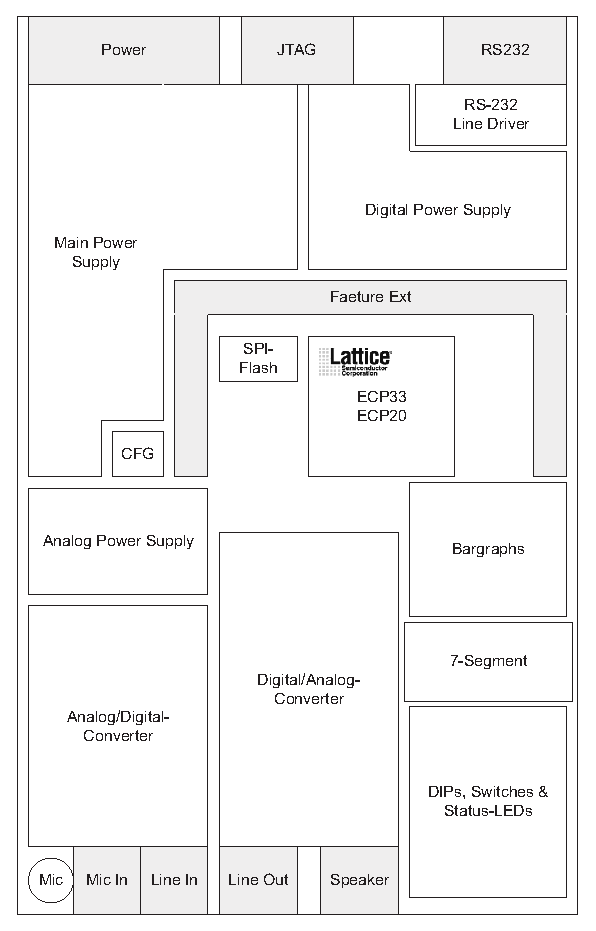
\includegraphics[scale=0.80]{Einfuehrung/bilder/ADS-Praktikum_Leiterplatte_BW.eps}}
	\caption{ADSP-SPATES}
	\label{fig:ADS-Praktikum Leiterplatte}
\end{figure}

\pargraphbox{bilder/global/esd.eps} {Bei der Handhabung ist Vorsicht geboten. Es handelt sich fast ausschlie�lich um Bauteile in	CMOS Technologie.	Zwar besitzen die Schaltkreise inzwischen sehr gute ESD-Schutzschaltungen, dennoch k�nnen diese durch unsachgem��e Handhabung zerst�rt werden. Da die Bauteile teuer sind,	bitte vorher das PC-Geh�use anfassen und sich entladen. Dann sollte nichts passieren.}

Zuerst schalten sie Ihr Netzger�t ein und stellen beide Spannungen auf 15V. Wieder ausmachen und eine Br�cke wie in Abb. \ref{fig:power-short} einstecken, so dass 30V Versorgungsspannung anliegen. Mit dem Adapterkabel (vgl. Abb. \ref{fig:power-cable}) verbinden sie das Netzger�t mit dem SPATES. Der Stecker geht manchmal etwas schwerer, allerdings sollte man keine Gewalt oder ein Messer anwenden m�ssen.


\begin{figure}[ht]
	\centering
	\begin{minipage}[b]{.4\linewidth}
		\centering
		\includegraphics[height=20ex]{Einfuehrung/bilder/power_short.eps}
		\caption{Netzteil-Br�cke}
		\label{fig:power-short}
	\end{minipage}
	\begin{minipage}[b]{.4\linewidth}
	  \centering
		\includegraphics[height=10ex]{Einfuehrung/bilder/power_cable.eps}
		\caption{Power cable}
		\label{fig:power-cable}
	\end{minipage}
\end{figure}

Anschlie�end k�nnen sie das Netzteil wieder einschalten. Zuerst sollten ihnen die verschiedenen Versorgungsspannungs-LEDs auffallen, die eine Funktion der einzelnen Spannungsebenen signalisieren (oder eben auch nicht, dann beim Betreuer melden). Nach einem kurzen Bootvorgang, der durch 2 LEDs direkt neben dem FPGA signalisiert wird, startet auch schon das Diagnose-Programm. Hierbei werden alle LEDs, die 7-Segment-Anzeigen und die Bargraphs kurz angesteuert. Falls der Lautsprecher schon angeschlossen ist, m�sste danach ein kurzer Sweep\footnote{Durchfahren eines Frequenzbereichs z.B. 20Hz bis 20kHz} zu h�ren sein. Ist dieser Test abgeschlossen, so kann man interaktiv alle weiteren Bedienelemente testen. Dabei gilt die Zuordnung aus Tabelle \ref{tab:s2led-assignment}.

\begin{table}
	\centering
	\begin{tabular}{|c|c|}\hline
		\textbf{Schalter/Taster} & \textbf{Anzeigeelement}\\\hline
		S1 & Alle Segmente LD1 \\\hline
		S2 & Alle Segmente LD2 \\\hline
		S3 & Alle Segmente LD3 \\\hline
		S4 & Alle Segmente LD4 \\\hline
		S5 & Alle Segmente Bargraph 1,2 \\\hline
		S6 & Status 1R, 1Y, 1G \\\hline
		S7 & Status 2R, 2Y, 2G \\\hline
		S8 & Status 3R, 3Y, 3G \\\hline
		DIP 1-8 & Bargraph 1,2 LEDs 1-8 \\\hline
	\end{tabular}
	\caption{Zuordnungen der Taster und Schalter}
	\label{tab:s2led-assignment}
\end{table}
	
%	\part{Grundlegendes}\label{part:Basics}
%		\include{Basics/Basics}
	
% Sender
	
	\cleardoublepage

\part{Versuche}\label{part:Exercises}
	\thispagestyle{empty}
	\cleardoublepage
	
	\chapter{Sender}\label{chap:sender}
	\thispagestyle{empty}

	\begin{figure}
		\centering 
		%\psfrag{01}{MATLAB Workspace}
		\includegraphics[width=10cm]{bilder/sender/sender_blockschaltbild}
		\caption{Sender Blockschaltbild}
		\label{abb:sender_blockschaltbild}
		\index{Sender Blockschaltbild}
	\end{figure}

Mittels des in Abb. \ref{abb:sender_blockschaltbild} dargestellten Systems werden die zu �bertragenden Signale erzeugt. Es besteht aus einem Pseudo-Zufallszahlen-Generator, dessen Ausgangssignal mit Hilfe eines einfachen FSK-Modulators moduliert werden soll. Eine detailliertere Beschreibung der einzelnen Komponenten wird in den folgenden Kapiteln erarbeitet.
	% Die �bung Erste Schritte stellt einen einfachen Multiplexer dar

\section{Versuch 1: Erste Schritte}\label{sec:firststeps}
	\develnote{In diesem Teil bauen wir einen einfachen Multiplexer}

\subsection{Konzept}\label{subsec:firststeps:concept}

In diesem Versuch soll eine einfache Umschaltung von verschiedenen Quellen auf eine Senke realisieren. Es soll ein Signal aus 2 Sinusschwingungen, dem AD-Umsetzer und Stumm ausgew�hlt und dies auf den DA-Umsetzer durchgeschaltet werden k�nnen (vgl. Abb. \ref{fig:8-bit-4-to-1-mux}).

\begin{figure}[ht]
	\centering
		\includegraphics{bilder/sender/8-bit-4-to-1-mux}
	\caption{8-bit 4-zu-1-Multiplexer}
	\label{fig:8-bit-4-to-1-mux}
\end{figure}

\subsection{Realisierungsm�glichkeiten}\label{subsec:firststeps:possibilities}

Gruns�tzlich hat man in VHDL M�glichkeiten, getaktete (synchrone) und nicht getaktete (asynchrone) Vorg�nge zu beschreiben. Dazu ben�tigen wir wenige grundlegende Konstrukte. In vielen F�llen ist eine asynchrone Schaltung einfach durch ein Register am Ausgang in eine synchrone Schaltung umzuwandeln (vgl. Abb. \ref{fig:asynchron-synchron}). Man sollte allerdings bedenken, dass die Optimierung nur innerhalb einer Hierarchieebene effizient funktioniert. Wegen der besseren Testbarkeit wird der gesamte Code in Module gegliedert und eine Hierarchie aufgebaut. Die ist g�nstig f�r die Synthese und die Optimierungsalgorithmen die dieser zugrunde liegen. Werden nun lange Signalwege ohne Register �ber mehrere Modulgrenzen hinweggef�hrt, so kann der Algorithmus der Synthese nicht so effizient arbeiten. Daher sollten an den Grenzen der Module nach M�glichkeit Register verwendet werden. F�r weitere Informationen zur effizienten Programmierung, siehe \cite{hbecp}, Abschnitt "`HDL Synthesis Coding Guidelines for Lattice Semiconductor FPGAs"'. Diese Empfehlungen treffen nicht nur auf die FPGAs von Lattice zu, sondern sind allgemein anwendbar.

\begin{figure}[ht]
	\centering
		\includegraphics{bilder/sender/asynchron_synchron}
	\caption{Synchrone Schaltung}
	\label{fig:asynchron-synchron}
\end{figure}


\subsection{VHDL: Realisierung}\label{subsec:firststeps:vdhl:realisations}

\subsubsection{VHDL-Basics: Libraries}\label{subsec:vhdl:basics:libraries}

Libraries in VHDL dienen haupts�chlich zur Definition von Typen, Funktionen und f�r die Definition der Resolution Functions. Typen geben an, wie die Informationen eines Signals oder einer Variablen dargestellt werden und welchen Wertebereich diese besitzen. Funktionen sind vergleichbar den Funktionen in Software. Es ist m�glich sie mit Parametern aufzurufen und einen Wert zur�ck zu erhalten. Dies kommt beispielsweise bei der Umwandlung von Typen in andere zum Einsatz. Der meistgebr�uchlichste Typ bei der Beschreibung f�r FPGAs ist der std\_ulogic-\index{std\_ulogic} bzw. der std\_logic-Datentyp\index{std\_logic}, wobei der std\_ulogic unresolved\index{unresolved} und der std\_logic resolved\index{resolved} ist. Resolved bedeutet, dass es m�glich ist, ein Signal von mehreren Treibern ansteuern zu k�nnen, wie es bei einem Bussystem der Fall ist, unresolved Typen k�nnen hierzu nicht verwendet werden. Die m�glichen Werte der beiden genannten Typen sind Tabelle \ref{tab:std-logic} zu entnehmen.

\begin{table}[ht]
	\centering
	\begin{tabular}{|c|c|l|} \hline
		\textbf{Wert} & \textbf{Bezeichnung} & \textbf{Erkl�rung} \\ \hline
		\textbf{'U'} & Not initialized 	& Dem Signal wurde noch kein Wert zugewiesen \\
		\textbf{'X'} & Forcing Unknown 	& Das Signal wird gegenl�ufig getrieben \\
		\textbf{'0'} & Forcing 0 				& Dies entspricht einem LOW-Pegel \\
		\textbf{'1'} & Forcing 1 				& Dies entspricht einem HIGH-Pegel \\
		\textbf{'Z'} & High Impedance 	& Das Signal wird nicht getrieben \\
		\textbf{'W'} & Weak Unknown 		& Das Signal wird schwach auf Unknown gehalten \\
		\textbf{'L'} & Weak 0 					& Das Signal wird schwach auf LOW-Pegel gehalten \\
		\textbf{'H'} & Weak 1 					& Das Signal wird schwach auf HIGH-Pegel gehalten \\
		\textbf{'-'} & Don't care 			& Der Wert des Signals ist zu ignorieren \\\hline
	\end{tabular}
	\caption{Der Typ std\_logic}
	\label{tab:std-logic}
\end{table}

Diese Werte sind in der Library \texttt{ieee.std\_logic\_1164} definiert. Einige weitere wichtige Libraries werden im Folgenden in die Projekte eingebunden:

\begin{verbatim}
library ieee
use ieee.std_logic_1164.all;
use ieee.std_logic_arith.all;
use ieee.std_logic_signed.all;
use ieee.numeric_bit.all;
\end{verbatim}

Teilweise kann deren Quellcode in den Dateien, welche vom Herstellertool mitgeliefert wurden, eingesehen werden. Bei ispLEVER sind diese im Verzeichnis \\ \verb|C:\ispTOOLS5_1\synpbase\lib\vhd\| \\ zu finden.

Weitere Typen lernen Sie zu gegebener Zeit kennen.

\subsubsection{VHDL-Basics: Die Entity}\label{subsec:vhdlbasics:entity}

Da der Multiplexer angeschlossen werden muss, definieren wir eine entity, die gerne mit dem Sockel eines ICs verglichen wird. Eine Entity wird folgenderma�en beschrieben:

\begin{verbatim}
entity <NAME> is
	
	[generic ( <VARNAME>: <VARTYPE> := <STD_VALUE>[; <VARNAME> ...]);]
	port ( <SIGNAL>: <DIRECTION> <TYPE>[; <SIGNAL>:]);

end;		
\end{verbatim}

F�r die \textit{DIRECTION}\footnote{Signalrichtung} sind vorl�ufig nur \texttt{in} und \texttt{out} interessant.

Damit ist festgelegt, wie ein Modul aussieht und einzubinden ist. Die Generics dienen dazu, das Modul konfigurierbar zu machen und sind nicht notwendig, der \textit{port} hingegen beschreibt die Pins und ist somit unabdingbar. Um nicht jedes Bit einzeln verdrahten zu mussen, wirde ein weiterer Typ eingef�hrt: std\_logic\_vector

Dabei handelt es sich um ein Array von std\_logic mit dem ein einfacher Bus dargestellt werden. Die Gr��e dieses Arrays kann folgenderma�en festgelegt werden:

\begin{verbatim}
...
  my_bus: in std_logic_vector(31 downto 0);
...
\end{verbatim}

\advise{�blicherweise werden Vektoren immer absteigend definiert (MSB soll links sein, auch bekannt als \textit{little endian}). Im Praktikum wollen wir uns deshalb auf \texttt{downto} beschr�nken.}

\subsubsection{VHDL-Basics: Die Architecture}\label{subsec:vhdlbasics:architecture}

Die \textit{architecture} wird ben�tigt, um der Entity Leben einzuhauchen. Mit VHDL beschreibt man, wie sich das Modul verhalten soll. Bisher wurden nur die Anschl�sse definiert.

\begin{verbatim}
architecture <NAME> of <ENTITYNAME> is
  [DECLARATIONS]
begin
  [INSTANTIATIONS]
end;
\end{verbatim}

In Fall des Multiplexers bekommt diese den Namen \textit{multiplexer\_behavioral} und die Entity \textit{my\_multiplexer}. F�r die Simulation sind hier in der Beschreibung keine Grenzen gesetzt, solange es sich um korrekte VHDL-Syntax handelt. Will man die Beschreibung jedoch synthetisieren und implementieren\footnote{Abrebitsschritte vom VHDL-Code zur lauff�higen Hardwarearchitektur}, so m�ssen bestimmte Regeln eingehalten werden. Diese Regeln sind jedoch von Tool zu Tool unterschiedlich. Unter Umst�nden ist es mit manchen Tools m�glich, eigentlich unerlaubte Anweisungen dennoch mit vielen Tricks in lauff�hige Hardware umzusetzen. Es sollte jedoch unbedingt auf diese Tricks verzichtet werden, da die Portabilit�t, Zuverl�ssigkeit und auch die Geschwindigkeit stark darunter leiden k�nnen.

\subsubsection{VHDL-Basics: Concurrent Statements}\label{subsec:vhdlbasics:concurrent}

Generell gibt es, wie weiter oben erw�hnt, bei digitaler Hardware zwei Vorgehensweisen: Asynchron und synchron. Der Multiplexer ist im einfachsten Fall eine asynchrone Schaltung. Diese ansynchronen Teile bezeichnet man in VHDL als \texttt{concurrent statement}, da diese nebenl�ufig, also alle gleichzeitig, abgearbeitet werden.

Ein solches Statement schreibt man direkt in die architecture. Dem linken Teil wird das Ergebnis des rechten Teils zugewiesen.

\begin{samepage}
\begin{verbatim}
...
  OUT_1 <= IN_1;           -- Einfache Verbindung
  OUT_2 <= IN_1 or IN_2;   -- Logische ODER-Verkn�pfung
  OUT_3 <= not IN_3;       -- Invertierung
...
\end{verbatim}
\end{samepage}

Weiterhin stehen Ihnen alle nachfolgenden logischen Operationen zur Verf�gung.

\begin{description}
	\item[xor] Verkn�pft den linken mit dem rechten Ausdruck �ber die XOR-Funktion
	\item[and] Eine UND-Verkn�pfung des linken und rechten Ausdrucks
	\item[or] Die ODER-Verkn�pfung
	\item[not] Invertiert den rechts stehenden Ausdruck
\end{description}

\advise{Auch \textit{concurrent statements} haben eine Verz�gerung, wenn Logik im rechten Anweisungsteil enthalten ist.}	

In Concurrent Statements k�nnen auch Multiplexer realisiert werden.

\begin{samepage}
\begin{verbatim}
...
  OUT_1 <= IN_1 when SEL_1 = '1' else 
           IN_2 when SEL_2 = '1' else '0';
...
\end{verbatim}
\end{samepage}

\subsection{VHDL: Beschreibung der Hardware}\label{subsec:firststeps:HWdesc}

\paragraph{Aufgabe 1}

Zun�chst soll ein Multiplexer in VHDL implementiert werden. Sie finden einen vorbereiteten Code-Rahmen im Verzeichnis \verb|01_Multiplexer\my_multiplexer.vhd|.
Der Abschnitt, der in der Datei mit \verb|--WRITE HERE| bezeichnet ist, soll durch Ihren Code ersetzt werden.

\develnote{cordic durch DSS in Abb. \ref{fig:multiplexer-toplevel} ersetzen}

\begin{figure}[ht]
	\centering
		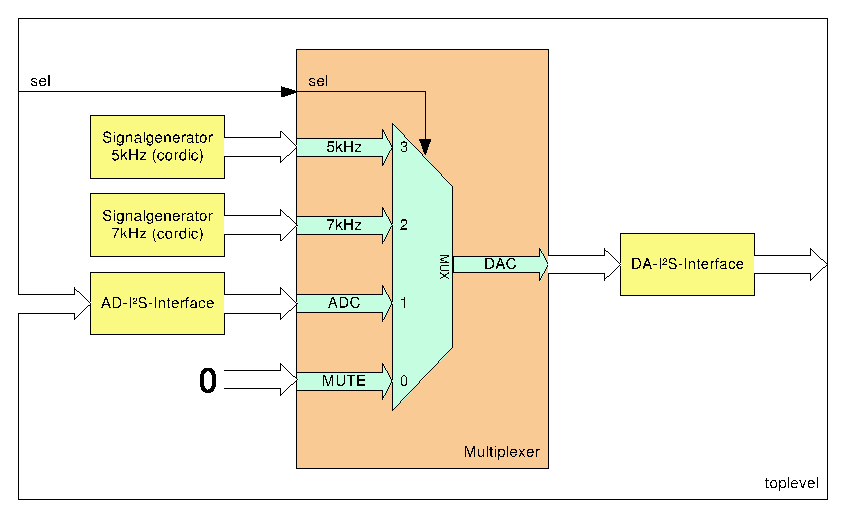
\includegraphics[width=0.85\textwidth]{bilder/sender/Multiplexer_toplevel.eps}
	\caption{Der Toplevel des Multiplexers}
	\label{fig:multiplexer-toplevel}
\end{figure}

\subsection{VHDL: Implementierung in Hardware}\label{subsec:firststeps:HWimplement}

Um den VHDL-Code auf dem FPGA auszuf�hren, muss die Beschreibung auf die FPGA-spezifische Technologie abgebildet, also �bersetzt werden. Dies erledigt das Synthese-Tool von ispLEVER.

\paragraph{Aufgabe 2:}

Speichern sie alle ge�ffneten Dateien. Anschlie�end lassen sie das Projekt synthetisieren, indem sie das Toplevel ausw�hlen und den Prozess \\

\includegraphics{bilder/sender/ispLeverSynthesize} im Aktionsbereich der Oberfl�che starten. Synplify erzeugt eine Netzliste, mit der ispLEVER weiterarbeiten kann. Sind keine Fehler aufgetreten, w�hlen sie im Hierarchie-Fenster das FPGA 
\includegraphics{bilder/sender/hirarchy_fpga.eps} aus. F�r die Programmierung wird ein Bitstream ben�tigt, den sie auf die Hardware �bertragen k�nnen. W�hlen sie die Aktion \includegraphics{bilder/sender/process_generate_bitstream_data.eps} aus, so f�hrt ispLEVER alle notendigen Prozesse in der richtigen Reihenfolge aus, und erzeugt das Bitfile.

\subsection{TEST: Praxis}\label{subsec:firststeps:test}

\paragraph{Aufgabe 3:}

�bertragen sie das Bitfile in das FPGA. Dazu starten sie das Programm ispVM  (Symbol  \includegraphics[width=1.5em]{bilder/sender/ispVM_symbol.eps} in der Toolbar). (s. Abb \ref{fig:ispVM-window})

\begin{figure}[ht]
	\centering
		\includegraphics[width=0.85\textwidth]{bilder/sender/ispVM_window.eps}
	\caption{Das ispVM-Fenster}
	\label{fig:ispVM-window}
\end{figure}

\develnote{TODO}

	\section{Versuch 2: Zufallsfolgengenerator}\label{sec:randomize}

%
%
%\subsection{PRN-Schieberegister}
%
%

\subsection{Konzept}\label{subsec:randomize:idea}

Zur Validierung von digitalen Schaltungen ist es oft w�nschenswert, die Stimuli\footnote{Steuernde Eingabe eines Systems} m�glichst zuf�llig aber dennoch reproduzierbar zu erzeugen. Durch die zuf�lligen Folgen wird so eine m�glichst gleichm��ige Verteilung �ber den Wertebereich erreicht, der eine gute Testabdeckung\footnote{Testabdeckung beschreibt das Verh�ltnis von m�glichen Fehlern zu den getesteten Zust�nden}\index{Testabdeckung} erm�glicht. Durch Verwendung von Pseudo-Zufallsfolgen-Generatoren k�nnen somit die zu erwartenden Ergebnisse allein durch Kenntnis des Startwertes ermittelt werden.


\subsection{Realisierungsm�glichkeiten}\label{subsec:randomize:possibilities}

Es gibt verschiedene M�glichkeiten eine sich st�ndig wiederholende Zufallsfolge zu erzeugen. Im einfachsten Fall generiert man einen Vektor, der die gew�nschte Folge enth�lt und ruft ihn immer wieder auf. Zugegebenerma�en ist diese Methode alles andere als elegant. Im Praktikum werden wir eine sch�nere M�glichkeit verwenden, indem wir PRN-Sequenzen\footnote{Pseudo-Random-Noise Sequenzen}\index{PRN-Sequenz} durch ein Schieberegister erzeugen lassen.

\subsubsection{PRN-Schieberegister}\index{PRN-Schieberegister}\label{subsec:randomize:prnshiftreg}

PRN-Sequenzen sind keine echten Zufallszahlen, sondern pseudo Zufallszahlen. Es sind Signale, die den Anschein einer zuf�lligen Folge von Nullen und Einsen erwecken, aber - bei der gleichen Anfangsbelegung der Schieberegister - reproduzierbare Ergebnisse liefern. Diese Tatsache kann man sich sp�ter zur Validierung der empfangenen Daten zunutze machen.

Zur Erzeugung der PRN-Folgen greifen wir auf ein N-Bit-Schieberegister zur�ck, bei dem der Eingang durch eine XOR-Verkn�pfung aus beliebigen Bits des Schieberegisters gebildet wird (vgl. Abb. \ref{abb:prnschieberegister}).

\begin{figure}[ht]
	\centering 
	%\psfrag{01}{MATLAB Workspace}
	\includegraphics[width=10cm]{bilder/sender/prn_register}
	\caption{PRN-Schieberegister}
	\label{abb:prnschieberegister}\index{PRN-Schieberegister}
\end{figure}

Auf diese Weise l�sst sich mit einem N-Bit-Schieberegister eine $2^N-1$ Bit lange Folge erzeugen. Wie man gut im Beispiel auf Seite \pageref{abb:prnschieberegisterbsp} erkennen kann, beginnt das Register nach einem vollst�ndigen Durchlauf wieder von vorne (siehe Abb. \ref{abb:prnschieberegisterbsp}). Anwendung in der Praxis findet diese Technik zum Beispiel beim Satellitenortungssystem GPS\footnote{GPS - Global Positioning System} zur Erzeugung der CA-Codes\footnote{Verwendet zur Identifizierung einzelner Satelliten} der einzelnen Satelliten (Detailierte Informationen zur Verwendung in GPS \cite{satnav}). 

\begin{figure}[ht]
	\centering 
	\psfrag{01}{Initialisierung}
	\psfrag{02}{Schritt 1}
	\psfrag{03}{Schritt 2}
	\psfrag{04}{Schritt $2^N-1$}
	\psfrag{05}{t}
	\includegraphics[width=10cm]{bilder/sender/prn_register_bsp}
	\caption{PRN-Schieberegisterdurchlauf}
	\label{abb:prnschieberegisterbsp}
\end{figure}

%
%
\subsection{MATLAB: Programmierung}\label{subsec:randomize:matlab:prn}
%
%

\paragraph{Vorbemerkung zur MATLAB-Programmierung:}
Um ein Gef�hl f�r MATLAB zu bekommen werden sie in den ersten Versuchen den Gro�teil der Skripte und Funktionen vorgegeben bekommen und nur die wichtigen Stellen selbst programmieren m�ssen. Da sie aber den Umgang mit MATLAB erlernen sollen, werden sie im weiteren Verlauf des Praktikums immer mehr dazu angehalten werden, die notwendigen Skripte und Funktionen selbst zu erstellen. Die ersten Versuche sollen ihnen hierf�r als anschauliches Beispiel dienen.

\paragraph{Los geht�s mit den ersten Gehversuchen in MATLAB:}
Vervollst�ndigen sie die im Verzeichnis \pathtomatlab{sender\textbackslash PRNSequenzgenerator} vorliegende MATLAB-Funktion \textit{PRNseq.m}, mit deren Hilfe - wie oben beschrieben - ein pseudozuf�lliger Datenstrom erzeugt werden kann.

�berpr�fen sie die Arbeitsweise ihrer Funktion, indem sie diese in einem MATLAB-Skript aufrufen, ihr die n�tigen Parameter �bergeben und sich den ausgegebenen Vektor als Balkendiagramm darstellen lassen. Dies erreichen sie in MATLAB mit der Plot-Funktion \textit{bar.m}. 

Lassen sie sich au�erdem die Anzahl der ausgegebenen Einsen und Nullen im Com\-mand-Win\-dow anzeigen.

\subsection{VHDL: Realisierung}\label{subsec:randomize:vhdl}

%
%
\subsubsection{VHDL-Basics: Signale}\label{subsec:vhdlbasics:signals}
%
%

Bisher wuden ausschlie�lich Signale verwendet, die durch die Entity bereits vorgegeben bzw. deklariert waren. Sogenannte Signale erm�glichen es, neue Namen zu definieren, die dann mit Werten belegt werden k�nnen. F�r den Anfang werden lediglich die zwei schon bekannten Typen ben�tigt.

\advise{Bei der Bezeichnung der Signale empfiehlt es sich, dem Signalnamen ein K�rzel voranzustellen, welches Auskunft �ber dessen Typ gibt. Alle Signale sollten klein geschrieben werden, um sie besser von Ports unterscheiden zu k�nnen.}

\begin{table}[hb]
	\centering
	\begin{tabular}{|cl|}\hline
		\emph{Pr�fix} & \emph{Bedeutung} \\ \hline
		sl & \textbf{\textcolor{red}{S}}ignal std\_\textbf{\textcolor{red}{l}}ogic \\
		sv & \textbf{\textcolor{red}{S}}ignal std\_logic\_\textbf{\textcolor{red}{v}}ector \\ \hline
	\end{tabular}
	\label{tab:typeprefixes}
	\caption{Vorgeschlagene Pr�fixe der bisher bekannten Typen}
\end{table}

Um einem Vektor einen Wert zuweisen zu k�nnen, wird eine M�glichkeit ben�tigt, Arrayelemente verkn�pfen zu k�nnen, um nicht jedem Element in einer eigenen Anweisung einen Wert zuweisen zu m�ssen. Hierzu gibt es mehrere M�glichkeiten, von denen je nach Anwendungsfall die geeignete auszuw�hlen ist.

\begin{verbatim}
...
architecture ...
...
  signal sv_bus: std_logic_vector(2 downto 0);
begin
...
  sv_bus(0) <= '1';
  sv_bus <= (others => '1'); -- Allen Elementen wird '1' zugewiesen
  sv_bus <= "010";           
  sv_bus <= '1' & '0' & '1';
  sv_bus <= '0' & "01"
  sv_bus(2 downto 1) <= "01";
...
end;
\end{verbatim}

Signale haben in der gesamten architecture G�ltigkeit. 

\subsubsection{VHDL-Basics: Sequentielle Prozesse}\label{subsec:vhdlbasics:seqprocesses}

Prozesse sind Teile des Sourcecodes, die synchron ablaufen sollen. Bisher wurden lediglich asynchrone Konstrukte (concurrent statements) verwendet. Besagte Prozesse sind im Grunde nichts anderes als ein gro�es concurrent statement. Mehrere Prozesse sind daher zueinander nebenl�ufig, werden also gleichzeitig ausgef�hrt.

\advise{Prozesse sind nicht vergleichbar mit Programmteilen aus dem Software-Sektor, in denen jeder Befehl nacheinander abgearbeitet wird. In Prozessen passiert alles gleichzeitig!}

Ein Prozess wird wie folgt beschrieben:

\begin{verbatim}
...
  [<name> :] process [(<SIGNAL1>, <SIGNAL2>)]
  begin
...
    -- CODE
...
  end;
...
\end{verbatim}

Der Name des Prozesses ist optional. Die sogenannte \textit{sensitivity list}\footnote{sensitivity list: Signalnamen in Klammern hinter \emph{process}. Bedingte Abarbeitung des Prozesses in der Simulation, bedingt durch die aufgef�hrten Signale.} gibt die Signale an, auf die der Prozess reagieren soll. Dies ist lediglich f�r die Simulation von Bedeutung, die den Prozess nur dann abarbeitet, wenn eines der genannten Signale seinen Wert �ndert, die Synthese beachtet diese Liste nicht sondern orientiert sich am Code im Prozess selbst.

Um den Prozess synchron auszuf�hren, ben�tigt man noch ein Clock- und ggf. ein Reset-Signal. Jeder sequentielle Prozess reagiert zumindest die Flanken�nderung des Clock-Signals. Ein Reset ist optional, sollte aber verwendet werden, um einen definierten Zustand nach dem Einschalten zu erhalten.

Ein typischer sequentieller Prozess sieht folgenderma�en aus:

\begin{verbatim}
...
  seq_proc : process (CLK, nRESET)
  begin
    if nRESET = '0' then
      -- CODE
    elseif rising_edge(CLK) then
      -- CODE
    end if;
  end;
\end{verbatim}

\advise{Meist verwendet man einen invertierten RESET. Dies folgt daraus, dass alle Signale im Einschaltzustand �blicherweise '0'-Pegel besitzen. Diese Invertierung kennzeichnet man gew�hnlich durch das "`n"' vor dem Signalnamen. Es stellt eine weitere freiwillige, aber sinnvolle Konvention f�r die Programmierung in VHDL dar.}

Alternativ f�r das oben verwendete \textit{rising\_edge}-Makro, wird manchmal folgendes schlechter lesbare Konstrukt eingesetzt:

\begin{verbatim}
...
    elsif CLK'event and CLK = '1' then
...
\end{verbatim}

Dies folgt daraus, dass einige Tools das \textit{rising\_edge}-Marko nicht kennen. Sollte bei der Synthese aufgrund dieses Makros ein Fehler auftreten, wenden sie sich bitte an den Betreuer. Die Meldung m�sste aussagen, dass die Synthese diese Funktion nicht kennt.

\advise{Wir verwenden in unserem Praktikum das Makro \textit{rising\_edge} um die Lesbarkeit des Codes zu verbessern.}

\subsubsection{VHDL-Basics: if-then-else}\label{subsec:vhdlbasics:ifthenelse}

Im vorherigen Abschnitt wurde bereits das if-then-else-Konstrukt verwendet. Dies ist nicht nur f�r die Clock-Flanken-Erkennung n�tzlich sondern erm�glicht auch das Programmieren bedingter Zuweisungen. Allerdings ist es nur in Prozessen zul�ssig. In concurrent statements muss man sich auf when-else, wie beim Multiplexer verwendet wurde.

Das if-then-else-Konstrukt ist wie folgt definiert:

\begin{verbatim}
...
  if <BEDINGUNG> then
    -- CODE
  [elsif <BEDINGUNG> then
    -- CODE ]
  [else
    -- CODE ]
  end if;
...
\end{verbatim}

\advise{Immer alle F�lle abdecken, ansonsten \emph{else} verwenden. Ausnahme: Clock-Flankenerkennung.}

\subsection{VHDL: Beschreibung der Hardware}\label{subsec:randomize:HWdesc}

\paragraph{Aufgabe 1: PRN-Schieberegister}

Es soll ein PRN-Schieberegister verwirklicht werden. In der Datei\\ \verb|02_Randomize\prn_shifter.vhd| \\
finden sie den ben�tigten, vorgefertigten Sourcecode, um ein solches PRN-Schieberegister zu programmieren. Das Register soll 16 Bit lang sein, und das XOR-Element soll zwischen Ausgang und der 6. Stelle eingef�gt werden (vgl. \ref{fig:PRN16}).

\begin{figure}
	\centering
		\includegraphics{bilder/sender/PRN16}
	\caption{16-stufiges Schieberegister mit XOR-R�ckkopplung}
	\label{fig:PRN16}
\end{figure}
\develnote{TODO: 16-Bit PRN-Schieberegister Grafik PRN16 einf�gen}

Als kleine Hilfestellung sei noch erw�hnt, dass sie Ausgabe-Ports (out) nur zuweisen, nicht jedoch lesen k�nnen. Es ist daher n�tig, ein Signal zu definieren, mit dem sie im Code arbeiten k�nnen und dem Ausgangs-Port dann den Wert dieses Signals zuzuweisen.

\paragraph{Aufgabe 2: Anfangszustand}

Welchen Anfangswert muss das Schieberegister haben bzw. darf es nicht haben, um die Funktion sicherzustellen
\answergame{5}{Nicht (others => '0'), um die Verifikation zu vereinfachen, sollte der Betreuer bei Fehlern die Studenten anweisen, den Anfangswert auf (others => '1') zu setzen. Dann ergibt sich die Folge: TODO

%\paragraph{Aufgabe 2: Definierter Anfangswert}
% Diese Aufgabe flog zugunsten des besseren Lerneffekts.
%
%Was passiert, wenn Sie den Anfangswert des Schieberegister auf \\ 
%\verb|(other => '0')|\\
%setzen?

\subsection{MODELSIM: Simulation der Beschreibung}\label{subsec:randomize:behavesim}

\subsubsection{Einf�hrung in Modelsim}\label{subsubsec:modelsim:introduction}

Modelsim ist ein Simulationstool, mit dessen Hilfe sie eine VHDL-Be\-schrei\-bung in praktisch jeder Abstraktionsebene durchf�hren k�nnen. Es unterst�tzt die be\-ha\-vioral-Be\-schrei\-bung, die syntetisierte Neztliste und auch die implementierte Beschreibung auf Gatterebene mit allen Timings. Es ist also eine vollst�ndige Simulation eines Moduls m�glich. Die Simulation der kompletten Hardware kann jedoch nur selten erfolgen, da einerseits die Stimuli oft nicht hinreichend genau bekannt sind und die Simulation selbst �u�erst viel Zeit und Rechenaufwand beanspruchen w�rde.

\advise{Einzelne Module k�nnen schnell mit der Simulation verifiziert werden. Komplette Hardware nur eingeschr�nkt bzw. gar nicht}

F�r die Simulation muss eine sogenannte Testbench generiert werden. Viele Hersteller-Tools besitzen daf�r ein grafisches Frontend mit, das jedoch bei weitem nicht die M�glichkeiten einer VHDL-Testbench bietet. Daher werden im Praktikum ausschlie�lich eine VHDL-Dateien verwendet, die keinerlei Ports nach au�en haben und das DUT\footnote{DUT: Device Under Test}, also unser Modul, als Komponente einbindet. Die Generierung der Stimuli und auch ggf. die Auswertung der Antworten erfolgt ebenfalls in VHDL. In der Simulation sind im Gegensatz zur Synthese alle VHDL-Konstrukte erlaubt, was es uns gestattet, auf einer sehr hohen Abstraktionsebene zu programmieren.

\ifthenelse{\xemacs}{% XEmacs wird verwendet !!!
Da wir als Editor XEmacs verwenden, k�nnen wir praktisch in wenigen Sekunden eine komplette Testbench bauen, da dieser Editor, wie beinahe f�r alle gr��eren Aufgabe, ein Template bereit stellt. Hierzu klicken wir in unserem Sourcefile mit der rechten Maustaste auf die Port-Deklaration und w�hlen im Men� \emph{Port$\rightarrow$Copy}. Anschlie�end erstellen wir die Testbench mit \emph{Port$\rightarrow$Paste as Testbench}

XEmacs erzeugt darufhin ein neues File mit dem Namen der Entity mit dem Zusatz \verb|_tb|, was auf deren Natur als Testbench hinweisen soll. Nach einigen Fragen, die von XEmacs gestellt werden, ist die Testbench fertig und bereit zur Verwendung. Einige kleine Korrekturen k�nnen noch n�tig sein. Meist ist das CLK-Signal zweimal deklariert. XEmacs generiert f�r jeden gemappten Port ein eigenes Signal. Das CLK-Signal ist jedoch intern auch schon in der Testbench deklariert und wird als globaler Clock verwendet. Durch auskommentieren einer dieser Deklarationen haben wir diesen Fehler schon beseitigt. Er tritt auf, weil man im Normalfall nicht den Namen CLK f�r den Clock in einem Modul verwendet sondern diesem besser einen aussagekr�ftigeren Namen gibt, der andeutet, woher dieser stammt (z.B. CLK\_ADC\_SCLK: Der Source-Clock f�r unseren ADC).
}{% XEmacs wird nicht verwendet!!!
Um nicht f�r jede zu testende Datei eine eigene Testbench bauen zu m�ssen, bietet die Entwicklungsumgebung von ispLEVER einen Testbench-Generator an, mit dessen Hilfe schnell eine eigene Testbench erzeugt werden kann. Dazu das zu testende VHDL-Modul im Hierarchie-Fenster von ispLEVER anw�hlen und im Aktionsfenster den Punkt 

\includegraphics{bilder/sender/ispLeverGenTestbench} ausw�hlen. Die Ausgabe im Fenster ist anschlie�end in eine Datei zu kopieren und mit geeigneten Stimuli zu versehen.}

Importieren sie nun die Testbench-Datei in ispLever,wobei sich diese unter dem zu testenden VHDL-File einordnet. Um Modelsim zu starten, w�hlen sie die Testbench in ispLever aus und starten sie die Aktion 
\includegraphics{bilder/sender/ispLeverSimulate}
wie in Abb. \ref{fig:simtestbench}

\begin{figure}
	\centering
		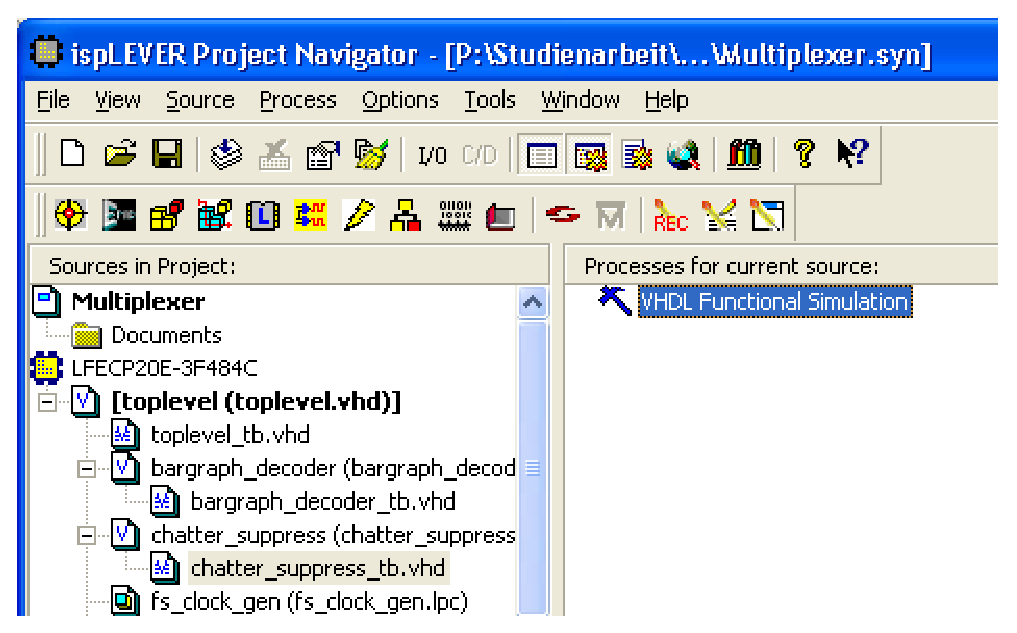
\includegraphics{bilder/sender/sim_testbench}
	\caption{Testbench simulieren}
	\label{fig:simtestbench}
\end{figure}

Nun startet Modelsim (vgl. Abb \ref{fig:modelsim}) und sie k�nnen anfangen, ihre Beschreibung zu simulieren. Mit den Standardeinstellungen gestartet, wird bereits $1 \mu s$ simuliert, sofern keine syntaktischen Fehler in der Beschreibung vorhanden sind. Sollte dies der Fall sein, so korrigieren sie die fehlerhafte VHDL-Datei und lassen sie diese erneut von Modelsim compilieren. Entweder sie schlie�en Modelsim und starten es �ber ispLEVER erneut oder sie recompilieren in Modelsim die Datei neu (vgl. Abb. \ref{fig:recompile}). Sie finden die Datei im Reiter \textbf{Work} im linken Teil des Modelsim-Fensters und mittels der rechten Maustaste erhalten sie ein Kontexmen� mit dem entsprechenden Befehl \textbf{recompile}. Anschlie�end sollten sie den Befehl \textbf{restart} ausw�hlen um die compilierten Versionen in den Speicher zu laden und erneut einen Zeitschritt mittels \textbf{run} simulieren lassen.

\begin{figure}
	\centering
		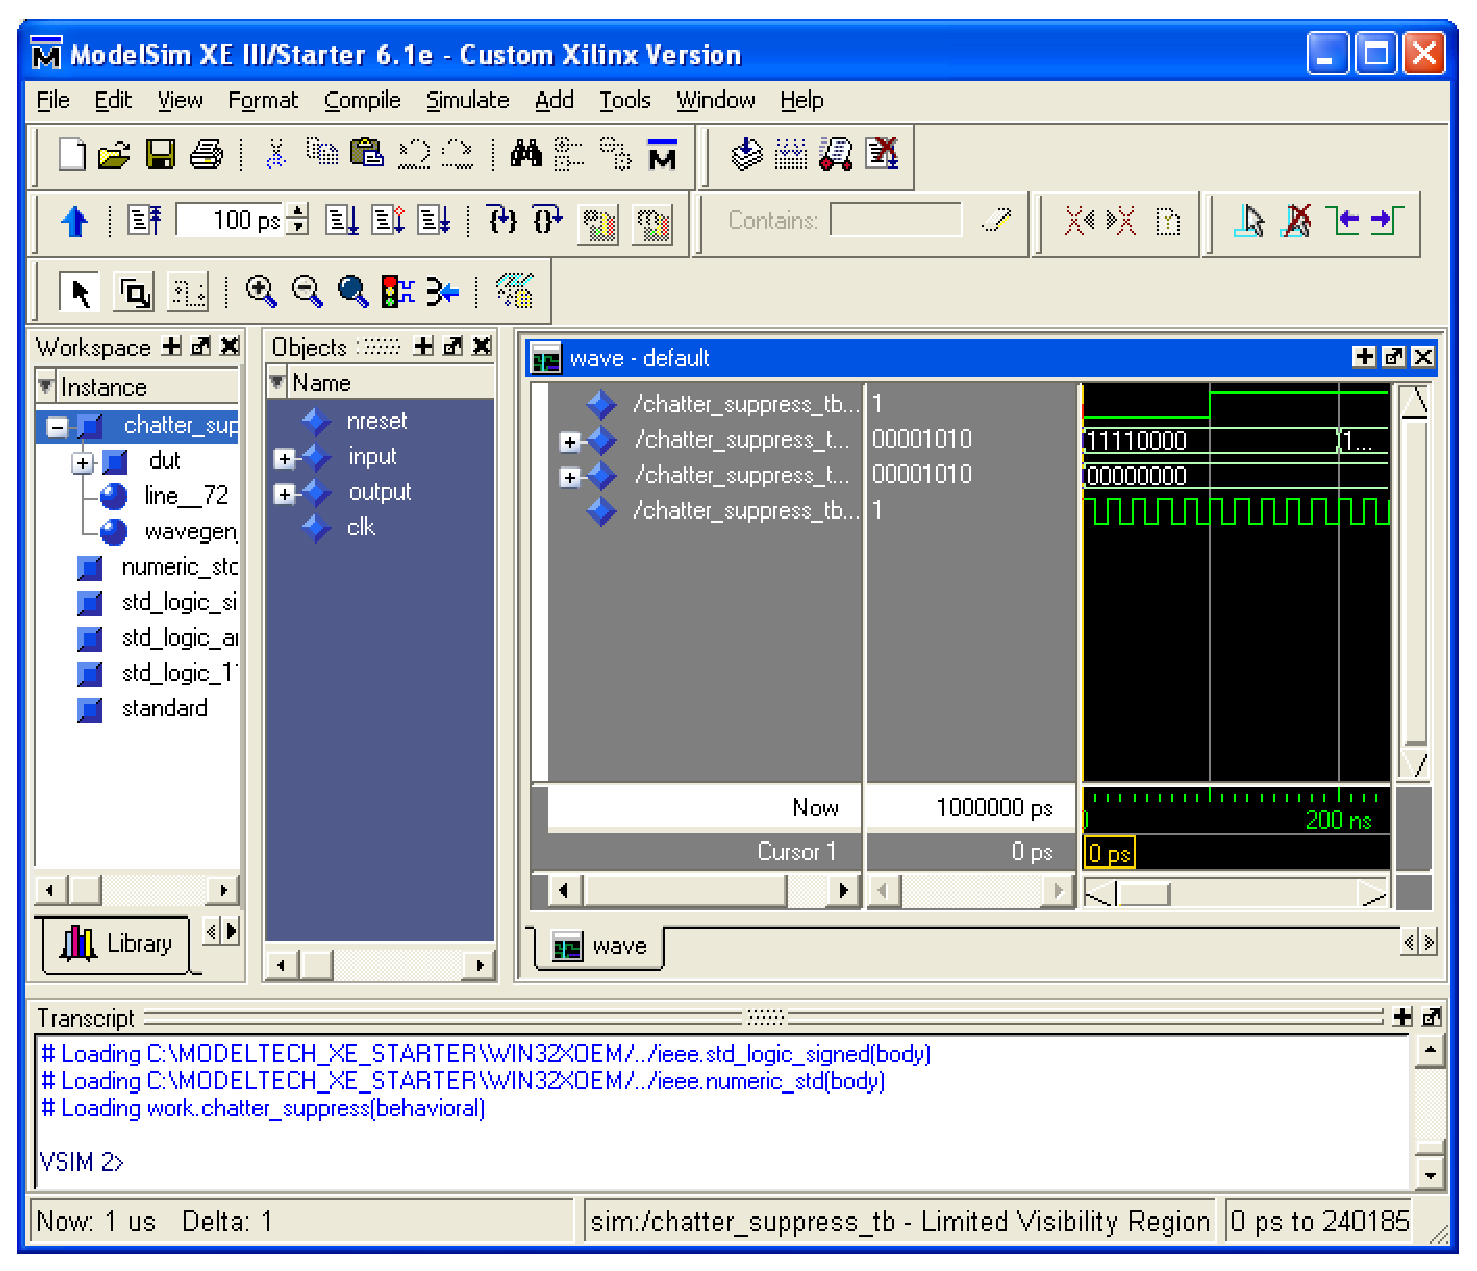
\includegraphics[width=0.95\textwidth]{bilder/sender/modelsim.eps}
	\caption{Modelsim nach dem Start mittels ispLEVER}
	\label{fig:modelsim}
\end{figure}

\begin{figure}
	\centering
		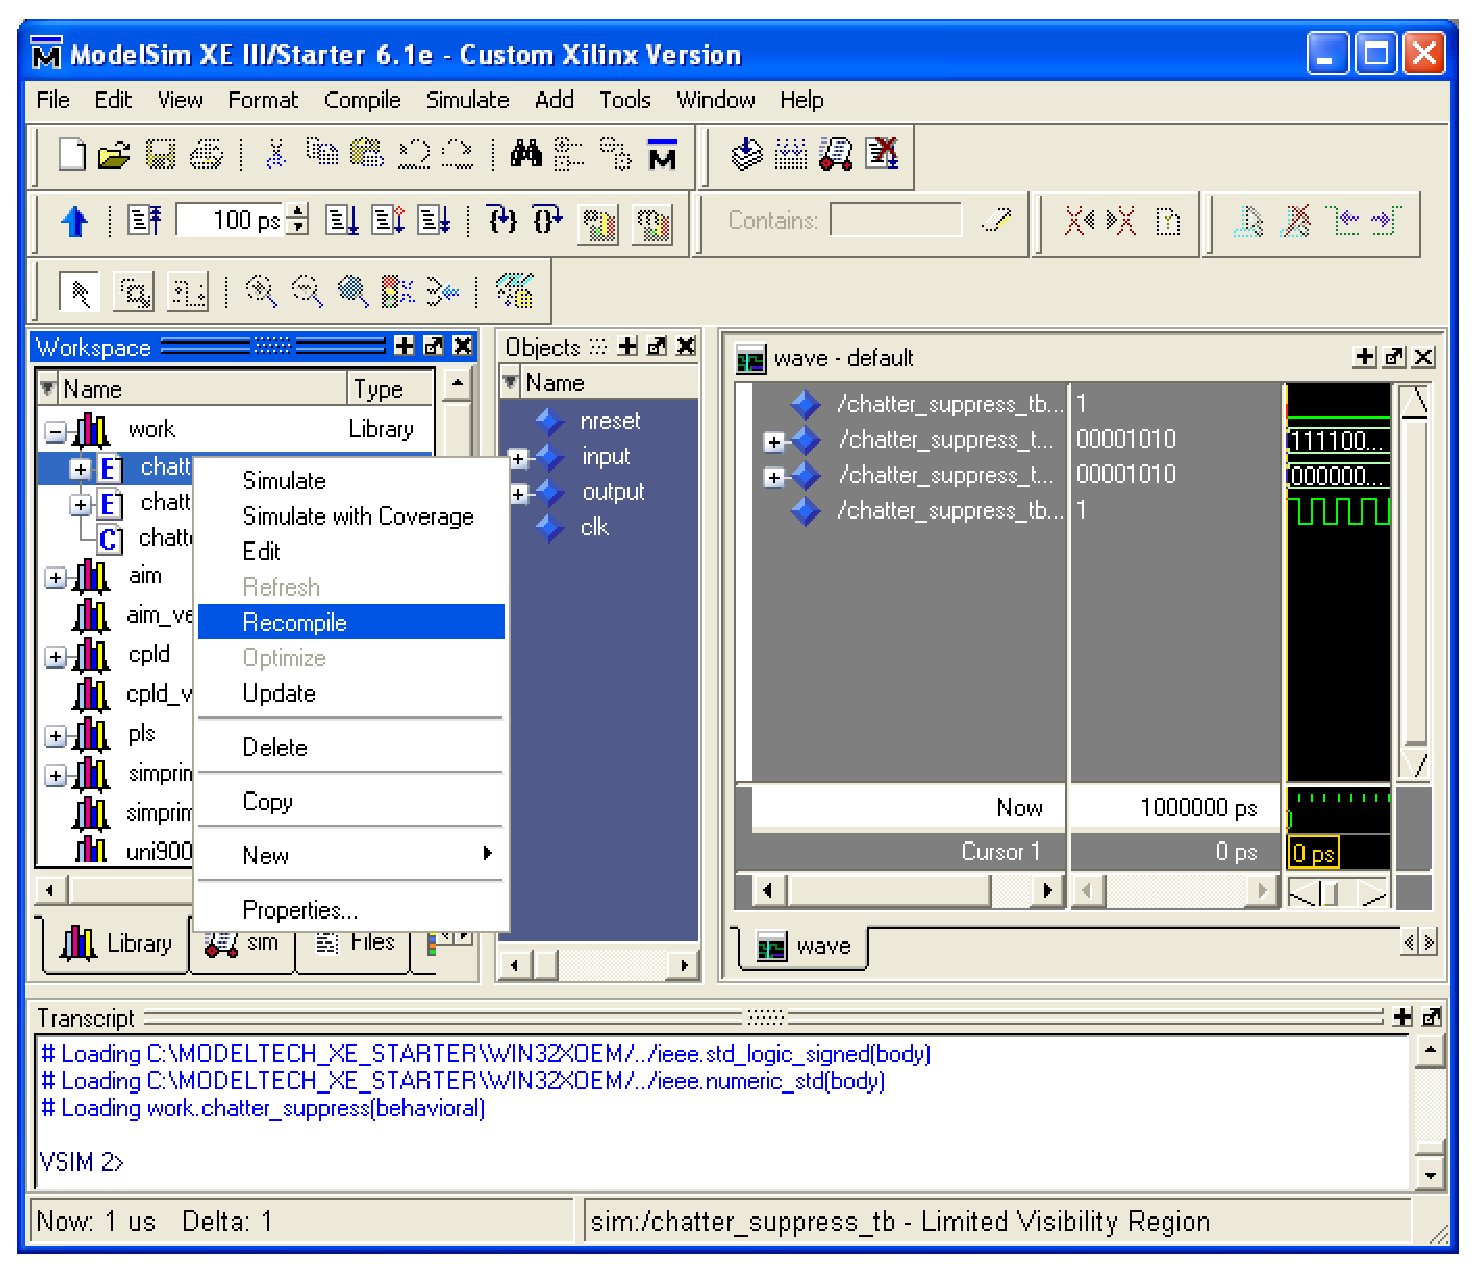
\includegraphics[width=0.95\textwidth]{bilder/sender/recompile.eps}
	\caption{Erneutes Compilieren einer VHDL-Datei}
	\label{fig:recompile}
\end{figure}

Alternativ k�nnen sie die Befehle auch in das Kommandofenster eintragen und mit Enter best�tigen bzw. mit \verb|;| mehrere Befehle voneinander Trennen. Mit der \keybutton{$\uparrow$}-Taste k�nnen sie die Historie der Befehle durchbl�ttern. So sind wiederkehrende Befehlsfolgen sehr einfach mit wenigen Tastendr�cken zu wiederholen. Beispielsweise mittels \\
\verb|vcom ...; restart; run 10 us| \\
mit einem Befehl, der in der Historie auch schnell wieder gefunden werden kann. 

Sollten sie noch weitere Fragen zu Modelsim haben, so wenden sie sich an den Betreuer. Eigentlich sollten keine Probleme mit der Bedienung von Modelsim entstehen. Behalten sie jedoch stets im Hinterkopf, dass Simulation und Hardware nur dann �bereinstimmen, wenn einerseits die Timings von der Synthese eingehalten werden k�nnen und andererseits die Simulation die von ihr ben�tigten Parameter auch erh�lt (z.B. die sensitivity list). W�rde man beispielsweise das Taktsignal nicht in die sensitivity list eintragen, dan w�re die Sumlation nicht funktionsf�hig, die Hardware w�rde allerdings ohne Einschr�nkungen funktionieren.

\paragraph{Aufgabe 3: Simulation}

Simulieren sie nun mit Hilfe der oben beschriebenen Prozedur den von ihnen programmierten Zufallszahlengenerator.

\subsection{TEST: Praxis}\label{subsec:randomize:test}

\paragraph{Aufgabe 4: Digitales Rauschen}

War ihre Simulation erfolgreich, so synthetisieren sie ihre Beschreibung und generieren sie das Bitfile.

Nun wird das generierte File in das FPGA geladen. Mit Hilfe des Tasters S1 kann ein Takt erzeugt werden, w�hrend der Inhalt des Schieberegisters HEX-Codiert auf den LED-7-Segment-Anzeigen dargestellt wird. Es besteht alternativ zum Taster die M�glichkeit, einen langsamen, automatisch generierten Takt mittels des Schalters 0 des 8-Dip-Switch zu aktivieren.

Jeweils 4 bit (ein BDC-Wort) wurden zu einer Stelle zusammengefasst. Die Anzeige stellt somit Werte zwischen 0 und F dar. Zus�tzlich werden alle Bits auf den Pegelanzeigen dargestellt. Die Linke bildet die niederwertigen (7 downto 0) Bits, die Rechte die h�herwertigen (15 downto 8).

\paragraph{Aufgabe 5: Qualit�t des Rauschens}

Schalten sie nun den automatischen Takt ein. Wie w�rden sie die Qualit�t des Rauschens beurteilen? Nur die letzte LED hat hierf�r eine Relevanz.

\answergame{4}{Das Rauschen ist gleichverteilt und der Zeitabstand zweier Wiederholungen sehr gro�. Somit ist das Rauschen von guter Qualit�t.}

	\section{Versuch 3: Signalgenerator}\label{sec:siggen}

\subsection{Konzepte}\label{subsec:siggen:concepts}

Um den erzeugten Bitstrom auf die �bertragung vorzubereiten muss man ihn, wie in Abbildung \ref{abb:sender_blockschaltbild} dargestellt, noch mit zwei Sinusschwingungen modulieren. Diese k�nnen im digitalen Bereich auf verschiedene Arten erzeugt werden. 

\subsection{Realisierungsm�glichkeiten}\label{subsec:siggen:possibilities}

Beispielhaft soll hier die Signalgenerierung mittels Direkter Digitaler Synthese (DDS)\index{DDS} und die Generation per CORDIC-Algorithmus\footnote{\underline{Co}ordinate \underline{Ro}tation \underline{Di}gital \underline{C}omputer}\index{CORDIC} besprochen werden. Beide Ans�tze f�hren zu unterschiedlichen Ergebnissen, worauf im Verlauf dieser Einf�hrung eingegangen werden soll.


%
\subsubsection{Direkte Digitale Synthese}\label{subsubsec:siggen:dds}
%

Die Direkte Digitale Synthese (DDS) ist ein Verfahren zur Erzeugung einer (meist periodischen) Funktion, deren Funktionswerte in einem Speicher, der Look-Up-Table\index{Look-Up-Table}(LUT\index{LUT}) abgelegt sind.

\paragraph{Einfache Variante:}
Die einfachste Variante besteht aus einem Z�hler oder S�gezahngenerator\index{S�gezahngenerator}, mit dessen Hilfe nacheinander die Zellen eines Speichers adressiert werden, in dem die Wertetabelle der einzelnen Signalwerte abgelegt ist. In Abbildung \ref{abb:dds01} ist der prinzipielle Aufbau dargestellt.
\begin{figure}[ht]
	\centering 
	%\psfrag{01}{MATLAB Workspace}
	\includegraphics[width=10cm]{bilder/sender/dds01}
	\caption{Direkte Digitale Synthese (DDS)}
	\label{abb:dds01}
\end{figure}

 Die Funktionswerte sind in der LUT abgelegt. Die Z�hlvariable $n$ adressiert den Speicher $i[n]=n+i_0$ und der ausgelesene Inhalt ergibt den gew�nschten Funktionswert $y[n]$. Ist die Z�hlvariable \textit{n} durch $w_{in}$ Bits und der Funktionswert \textit{y[n]} durch $w_{out}$ Bits repr�sentiert, so ben�tigt man (maximal)
\begin{equation}
	N_{Sp} = w_{out}2^{w_{in}}
\end{equation}
Speicherpl�tze. Mit jedem Takt der Abtastfrequenz $f_s$ wird der Z�hler inkrementiert. Kommt es zu einem �berlauf wird ein Statusbit gesetzt, worauf die Variable $n$ erh�ht wird und somit auf eine andere Speicherzelle zugegriffen wird.

\medskip Mit der oben beschriebenen Struktur sind 
\begin{itemize}
	\item nichtlineare Kennlinien (Anregung mit reinem Aufw�rtsz�hler) sowie 
	\item periodische Kennlinien (Anregung mit einer S�gezahnfunktion: Z�hler mit �berlauf)
\end{itemize}
realisierbar. 

\paragraph{Erweiterung:}
Will man Signale mit variablen Abtastfrequenzen und Periodendauern erzeugen ist es n�tig, die einfache Schaltung aus Abbildung \ref{abb:dds01} zu erweitern. Die modifizierte Schaltung ist in Abbildung \ref{abb:dds02} dargestellt.
\begin{figure}[ht]
	\centering 
	\psfrag{01}{$\Delta x$}
	\psfrag{02}{$x[n]$}
	\psfrag{03}{$i[n]$}
	\psfrag{04}{$y[n]$}
	\includegraphics[width=10cm]{bilder/sender/dds02}
	\caption{Erweiterte DDS}
	\label{abb:dds02}
\end{figure}

\subparagraph{Block 'Adresszuordnung':}\index{Adresszuordnung}
Der Block Adresszuordnung generiert zum diskreten Zeitpunkt $n$ eine Adresse $i[n]$, die angibt, welcher Funktionswert $y[n]$ von der LUT an den Ausgang gelegt werden soll. Die Adresse $i[n]$ wird durch das Intervall $\Delta x_i$ bestimmt, in dem sich der akkumulierte Phasenwert $x[n]$ befindet. 

\medskip Bei $2^{w_{in}}$ St�tzstellen kann man die Adresse unter der Annahme, dass das Argument $x[n]$ im Fractional-Format vorliegt folgenderma�en berechnen:
\begin{equation}
	i[n]=Q_{w_{in}}\left(2^{w_{in}-1}x[n]\right)+i_0
\end{equation}
$x[n]$ wird hierbei auf $w_{in}$ Stellen abgeschnitten. $i_0$ ist der Adressoffset und $Q_{w_{in}}$ die Quantisierungsfunktion, die das Argument auf $w_{in}$ Stellen vor dem Komma abschneidet.\\
\medskip \textbf{Beispiel zur Adresszuordnung:}
\begin{flushleft}
$w_{in}=4; x[n]=0.0010110, i_0=00001000$\\
$i[n]=0001. +00001000 = 00001001 (dezimal: i[n]= 1+8 = 9)$
\end{flushleft}

\subparagraph{Taktquelle:}\index{Taktquelle}
Die Taktquelle bestimmt die Abtastfrequenz des DDS-Systems. Die h�chste hier erzeugbare Signalfrequenz\footnote{vgl. Abtasttheorem} ist $\cfrac{f_s}{2}$.

\subparagraph{Phaseninkrement $\delta x$:}\index{Phaseninkrement}
Das Phaseninkrement bestimmt Phase und Frequenz des Ausgangssignals. Aufgrund der endlichen Wortbreite ($x_Q$) (LSB) k�nnen auch nur endliche Phasen-/ Frequenzaufl�sungen erreicht werden.
\begin{equation}
	\frac{\delta x}{N\delta x_i}=\frac{T_s}{T_0} \\
	\Longrightarrow T_{0Q}=\frac{\delta x_i}{\delta x_Q}NT_s \\
	\Longrightarrow f_{0Q}=\frac{\delta x_Q}{\delta x_i}\cdot\frac{1}{NT_s} 
\end{equation}

$N$ beschreibt hier die Anzahl der gespeicherten Abtastwerte pro Periode.

\subparagraph{Phasenakkumulator:}\index{Phasenakkumulator}
Der Phasenakkumulator ist nichts weiter als ein Addierer, der in jedem Taktzyklus einen vorgegebenen Wert $\Delta x$  aufaddiert. Die aktuelle Phasenlage berechnet sich zu
\begin{equation}
	x[n] = x[n-1] + \Delta x
\end{equation}
Der Wert Null steht hier f�r eine Phasenlage von 0\textdegree, sein Maximalwert f�r 360\textdegree. Somit liegt mit jedem Taktzyklus eine neue Phasenlage vor, die dann nur noch in einen Amplitudenwert umgerechnet werden muss.

\advise{Die Akkumulatorwortbreite muss stets gr��er oder gleich der Phaseninkrement-Wortbreite sein! Ist das nicht der Fall kommt es mit jeder Addition zu ungewollten �berl�ufen.}

\subparagraph{Signaltabelle -- Look-Up-Table (LUT):}\index{LUT}\index{Look-Up-Table}
Die Look-Up-Table ist ein Speicher, der eine endliche Anzahl Funktionswerte des zu generierenden, (oft) periodischen Signals in quantisierter Form enth�lt (Wortbreite $w_{out}$). Wegen der endlichen Wortbreite kommt es zu Quantisierungsfehlern. Ist die Phasenakkumulatorwortbreite gr��er als die Adressbreite der Signaltabelle, muss das Argument (die Phase) $x[n]$ gerundet werden. Als allgemeine Faustregel kann man sich merken, dass $w_{out}$ 2 Bit breiter als $w_{in}$ sein muss. 
Fehler treten auch auf, wenn zwischen den Tabellenwerten interpoliert wird, um die Ausgangswerte zu berechnen (Vorteil: Speicherplatzreduktion).

\medskip

Nachfolgend ein kurzes Beispiel zur erweiterten DDS: \\
Es soll mittels DDS ein Sinussignal ($y=\sin(\pi x)$ f�r $x\in[-1,1[$) erzeugt werden. Die verwendete LUT ist in Tabelle \ref{tab:dds_lut} dargestellt.

\begin{table}[ht]
	\centering		
	\begin{tabular}{|l|l|}\hline

			\textbf{x} & \textbf{y}\\\hline
			-1.0000 & 				0\\
			-0.8750	& -0.38269042968750\\
			-0.7500	& -0.70709228515625\\
			-0.6250	& -0.92388916015625\\
			-0.5000	& -1.00000000000000\\
			-0.3750	& -0.92388916015625\\
			-0.2500	& -0.70709228515625\\
			-0.1250	& -0.38269042968750\\
			 0			& 				0\\ 
			 0.1250	&  0.38269042968750\\
			 0.2500	&  0.70709228515625\\
			 0.3750	&  0.92388916015625\\
			 0.5000	&  1.00000000000000\\
		 	 0.6250	&  0.92388916015625\\
	 		 0.7500	&  0.70709228515625\\
 			 0.8750	&  0.38269042968750\\\hline																
	\end{tabular}
	\caption{DDS Look-Up-Table}
	\label{tab:dds_lut}
\end{table}

\develnote{Hier bitte das Beispiel auf Page210ff im ADS Skript noch einf�gen}

%
\subsubsection{CORDIC}\label{subsubsec:siggen:cordic}\index{CORDIC}
%

Wie sie im vorhergehenden Abschnitt erkennen konnten liefert die DDS zwar eine speicherplatzeffiziente, aber aufgrund der begrenzten Anzahl von Tabellenwerten relativ ungenaue L�sung. Daher wollen wir uns im Folgenden mit einer eleganteren und vielseitigeren Methode besch�ftigen: dem \textbf{CORDIC-Algorithmus}\footnote{CORDIC steht f�r ``Coordinate Rotation Digital Computer''}. Mit ihm lassen sich viele Berechnungen l�sen:
\begin{itemize}
	\item Im CORDIC-Basisverfahren\index{Basisverfahren} ist
	\begin{itemize}	
		\item die Berechnung der Drehung eines Vektors in einem kartesischen Koordinatensystem und die
		\item Berechnung von Betrag und Phase eines Vektors m�glich.
	\end{itemize}
	\item Im erweiterten CORDIC-Basisverfahren sind \index{erweitertes Basisverfahren}
	\begin{itemize}
		\item Multiplikation,
		\item Division und 
		\item Berechnung hyperbolischer Funktionen durchf�hrbar.
	\end{itemize}
\end{itemize}

Um eine Sinusschwingung zu erzeugen gen�gt es, sich mit dem CORDIC-Ba\-sis\-ver\-fah\-ren im Rotation-Mode\index{Rotation-Mode} auseinanderzusetzen. F�r erg�nzende Informationen zu den anderen Verfahren sei auf \cite{ADS} verwiesen.

\paragraph{Das CORDIC-Basisverfahren im Rotation Mode:}

Die Drehung eines Vek\-tors\\ $[x_0,y_0]^T$ um den Winkel $\theta$ in einem kartesischen Koordinatensystem f�hrt auf den Vektor $[x_n,y_n]^T$:
\begin{equation}
		\begin{bmatrix} x_n\\y_n\\ \end{bmatrix} = \begin{bmatrix} cos(\theta) & -sin(\theta)\\ sin(\theta) & cos(\theta)\\\end{bmatrix}\begin{bmatrix} x_0\\y_0\\ \end{bmatrix}
\end{equation}
In Abbildung \ref{abb:rot01} wird dies graphisch dargestellt.
\begin{figure}[ht]
	\centering 
	\psfrag{01}{$\theta$}
	\psfrag{02}{$(x_0,y_0)$}
	\psfrag{03}{$(x_n,y_n)$}
	\psfrag{04}{x}
	\psfrag{05}{y}
	\includegraphics[width=7cm]{bilder/sender/rot01}
	\caption{Drehung eines Vektors um den Winkel $\theta$}
	\label{abb:rot01}
\end{figure}
Unter Verwendung der Identit�t (aus Formel (\ref{math:ident}))
\begin{equation}
cos(\theta)=\cfrac{1}{\sqrt{1+tan^2(\theta)}} \textnormal{  und  } tan(\theta)=\cfrac{sin(\theta)}{cos(\theta)}
\label{math:ident}
\end{equation}
erh�lt man die Beziehung:
\begin{equation}
	\begin{bmatrix}x_n\\y_n\\\end{bmatrix}=\cfrac{1}{\sqrt{1+tan^2(\theta)}}\begin{bmatrix} 1 & -tan(\theta)\\ tan(\theta) & 1\\\end{bmatrix}\begin{bmatrix} x_0\\y_0\\ \end{bmatrix}
\end{equation}

Beim CORDIC-Verfahren wird die Drehung um $\theta$ durch mehrere Teilrotationen\index{Teilrotationen} mit bekanntem Teilwinkel $\alpha_i$ realisiert. Durch das festzulegende Vorzeichen $\sigma_i$ n�hert man die Summe der Teilwinkel $\alpha_i$ dem Winkel $\sigma$ an:
\begin{equation}
	\theta\approx\sum_{i=0}^{n-1}\sigma_i\alpha_i  \textnormal{ mit } \sigma_i \in\{-1,1\}
\end{equation}
Dies f�hrt zu der Beziehung
\begin{equation} 
	\begin{bmatrix}x_{i+1}\\y_{i+1}\\\end{bmatrix}=\cfrac{1}{\sqrt{1+tan^2(\alpha_i)}}\begin{bmatrix} 1 & 	-\sigma_i tan(\alpha_i)\\ \sigma_i tan(\alpha_i) & 1\\\end{bmatrix}\begin{bmatrix} x_i\\y_i\\ 					\end{bmatrix}
\end{equation}
f�r $i=0,1,...,n-1$.\\
Dabei wird $\alpha_i$ mit zunehmendem $i$ abnehmen. Zur Vereinfachung des Matrixprodukts und zur vereinfachten Umsetzung (in Hard- und Software) werden die $\alpha_i$ so gew�hlt, dass
\begin{equation}
	tan(\alpha_i)=2^{-i} \qquad i=0,1,...,n-1  \qquad (\alpha_i=arctan(2^{-i}))
\end{equation}
Damit werden die Multiplikationen mit $tan(\theta)$ zu Schiebeoperationen vereinfacht. Diese lassen sich in digitaler Hardware ohne gro�en Aufwand realisieren. \\Somit kann man schreiben:
\begin{equation}
 	\begin{bmatrix}x_{i+1}\\y_{i+1}\\\end{bmatrix}=k_i\begin{bmatrix} 1 & -\sigma_i 2^{-i}\\ \sigma_i 2^{-i} & 1\\\end{bmatrix}\begin{bmatrix} x_i\\y_i\\ \end{bmatrix} \textnormal{ mit } k_i=\cfrac{1}{\sqrt{1+2^{-2i}}}
\end{equation}
Die $\alpha_i$ werden positiv bewertet, bis die Summe den Wert von $\theta$ �berschreitet. Danach werden sie negativ bewertet, bis die Summe den Wert von $\theta$ wieder unterschreitet. Dies wird entsprechend fortgesetzt. Das Vorzeichen der Differenz
\begin{equation}
	z_{i+1}=\theta-\sum_{k=0}^i\sigma_k \alpha_k 
\end{equation}
steuert somit das Vorzeichen $\sigma_i$ der Teilwinkel. Die Hilfsvariable $z_i$ soll w�hrend des Iterationsprozesses gegen Null konvergieren (vergleiche Abb. \ref{abb:rot02}).

\begin{figure}[ht]
	\centering 
%	\psfrag{05}{y}
	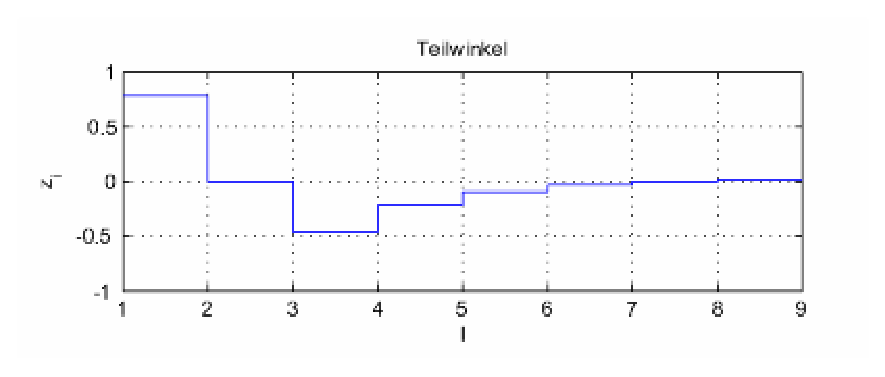
\includegraphics[width=11cm]{bilder/sender/rot02}
	\caption{Schrittweite der Variable $z_i$	}
	\label{abb:rot02}
\end{figure}

Die Werte f�r $\alpha_i=arctan(2^{-i})$ werden �blicherweise in Tabellenform abgelegt und werden schon im Vorfeld je nach gew�nschter Genauigkeit berechnet. Ein Beispiel ist in Tabelle \ref{tab:alphaiklut} angegeben.

\medskip Fasst man die Teilfaktoren $k_i$ f�r alle Iterationen zusammen, so ben�tigt man nur noch einen einzigen, abschlie�enden Skalierungsschritt, anstatt einzelner Multiplikationen nach jedem Iterationsschritt: 
\begin{equation}
 k=\prod_{i=0}^{n-1}\cfrac{1}{\sqrt{1+2^{-2i}}}
\end{equation}
Auch der gew�nschte Skalierungsfaktor k kann vorab berechnet und abgelegt werden (vgl. Tabelle \ref{tab:alphaiklut}).

\begin{table}[ht]
	\centering		
	\begin{tabular}{|l|c|l|l|l|}\hline

			i & $\alpha_i=arctan(2^{-i})$ & $\alpha_i \textnormal{ in [�]}$ & $k_i$ & k\\\hline
			0 & 0.7854 & 45				&	0.7071	&	0.7071	\\
			1	& 0.4636 & 26.5651	&	0.8944	&	0.6325	\\
			2	& 0.2450 & 14.0362	&	0.9701	&	0.6136	\\
			3	& 0.1244 & 7.1250		&	0.9923	&	0.6076	\\
			4	& 0.0624 & 3.5763		&	0.9981	&	0.6074	\\
			5	& 0.0312 & 1.7899		&	0.9995	&	0.6073	\\
			6	& 0.0156 & 0.8952		&	0.9999	&	0.6073	\\
			7	& 0.0078 & 0.4476   &	1.0000	&	0.6073	\\
			8	& 0.0039 & 0.2238		&	1.0000	&	0.6073	\\ 
			9	& 0.0020 & 0.1119		&	1.0000	&	0.6073	\\
		 10	& 0.0010 & 0.0560		&	1.0000	&	0.6073	\\\hline																
	\end{tabular}
	\caption{Look-Up-Table f�r $\alpha_i$ und Skalierungsfaktor k}
	\label{tab:alphaiklut}
\end{table}

\clearpage
Mit den bisherigen Vereinbarungen gilt f�r die Iterationsgleichungen:

\begin{itemize}
	\item Initialisierung: \[ z_0=\theta \]

	\item F�r $i=0,1,...,n-1$:
		
		\begin{equation} 
			\sigma_i=\begin{cases} +1 \textnormal{ f�r } z_i\ge 0 \\ -1 \textnormal{ f�r } z_i < 0 									\end{cases}
		\end{equation}
		
		\begin{equation}\begin{split}
			x_{i+1} & =x_i-\sigma_i2^{-i}y_i \\ 
			y_{i+1} & =y_i+\sigma_i2^{-i}x_i \\ 
			z_{i+1} & =z_i-\sigma_i 						arctan(2^{-i})
		\end{split}\end{equation}
		
\end{itemize}

Zur Skalierung auf den korrekten Amplitudenwert ist nun noch eine abschlie�ende Multiplikation durchzuf�hren:

\begin{eqnarray}
	kx_n & \rightarrow & x_n \\ 
	ky_n & \rightarrow & y_n
\end{eqnarray}

\paragraph{Fassen wir zusammen:}

\medskip Wird $\sigma_i$ wie oben beschrieben bestimmt, so konvergiert $z_n \rightarrow 0$ und das Differenzengleichungssystem hat die L�sung:
\begin{equation}\begin{split}
	x_n & =x_0cos(\theta)-y_0sin(\theta) \\ 
	y_n & =y_0cos(\theta)+x_0sin(\theta)
\end{split}\end{equation}
Da dies der Drehung eines Zeigers $(x_0,y_0)$ um den Winkel $\theta$ nach $(x_n,y_n)$ entspricht, spricht man vom sogenannten \textbf{Rotationsmodus}\index{Rotationsmodus} des CORDIC-Algorithmus. 

Durch geeignete Wahl des Startwertes $(x_0,y_0)=(x_0,0)$ kann mit dieser Methode das Produkt eines skalaren Wertes mit dem Sinus bzw. dem Cosinus berechnet werden:
\begin{equation}\begin{split}
	x_n & =x_0cos(\theta)\\ 
	y_n & =y_0sin(\theta)
\end{split}\end{equation}
Mit der Wahl $(x_0,y_0)=(k,0)$ und ohne die sonst notwendige Skalierung mit k am Ende des Iterationsprozesses erh�lt man:
\begin{equation}\begin{split}
	x_n & =cos(\theta)\\ 
	y_n & =sin(\theta)
\end{split}\end{equation}
Der CORDIC-Basisalgorithmus eignet sich also im Rotationsmodus
\begin{itemize}
	\item zur Drehung eines Zeigers um einen vorgegebenen Winkel und
	\item zur Berechnung der Winkelfunktionen $sin$ und $cos$.
\end{itemize}


%
%
\subsection{MATLAB: Programmierung}\label{subsec:siggen:matlab}
%
%

\paragraph{Aufgabe 1: DDS}

\begin{enumerate}
\item Machen sie sich mit dem MATLAB-Skript zur Direkten Digitalen Synthese (\textit{dds.m}) vertraut\footnote{\pathtomatlab{sender\textbackslash Sinusgenerator\textbackslash DDS}}. 
\item Stellen sie verschiedene Schwingungsfrequenzen $f_0$ dar und drucken sie die gelieferten Plots f�r ihre Dokumentation aus.
\end{enumerate}

\paragraph{Aufgabe 2: CORDIC}

\begin{enumerate}
\item Machen sie sich mit der Funktion \textit{CORDIC.m}\footnote{\pathtomatlab{sender\textbackslash Sinusgenerator\textbackslash CORDIC}} vertraut und erg�nzen sie die fehlenden Abschnitte.
\item Schreiben sie ein MATLAB-Skript (\textit{CORDICsim.m}), mit dessen Hilfe sie ihre Funktion mit unterschiedlichen Parametern (Iterationsschritte, Drehwinkel, Startwerte) testen k�nnen. Was f�llt ihnen auf, wenn sie um Winkel gr��er 100� drehen lassen wollen? Wodurch wird dieser Effekt ausgel�st?

\answergame{6}{Bei Teilrotationen �ber 100\textdegree errechnet der CORDIC-Algorithmus einen falschen Wert. Dies liegt daran, dass sich sein maximaler Aktionsradius aus der Summe der m�glichen Einzelrotationen zusammensetzt. \\
So ergibt sich zum Beispiel f�r $n=16$: 
\[ \sum_{i=0}^{15} arctan(2^{-i}) \approx 100^{\circ}\]
Der Aktionsradius des Algorithmus liegt also etwa zwischen\\ $-100^{\circ}...100^{\circ}$.}

\item Stellen sie die Gr��en $\sigma_i$, $\alpha_i$ $(x_0,y_0)$ und $(x_n,y_n)$ mit Hilfe der MATLAB Plot-Funktionen anschaulich dar und drucken sie ihre Ergebnisse aus.
\item Erg�nzen sie die vorliegende Funktion dahingehend, dass auch Winkel >90� richtig verarbeitet werden k�nnen. 
\item Was f�llt ihnen hinsichtlich Rechenaufwand und Genauigkeit auf, wenn sie die beiden Algorithmen (DDS $\leftrightarrow$ CORDIC) miteinander vergleichen?
\answergame{3}{Die direkte digitale Synthese ist Rechenzeit- und Speicherplatzeffizient. Daf�r liefert der CORDIC wesentlich genauere Ergebnisse.}

\end{enumerate}

\paragraph{Aufgabe 3: Sinus-Generator}
\begin{enumerate}
\item Kopieren sie nun ihre Funktion \textit{cordic.m} in das Verzeichnis \pathtomatlab{sender\textbackslash 03\_Sinusgenerator\textbackslash Oszillator} Hier finden sie au�erdem noch das Grundger�st der Funktion \textit{oszillator.m}. Erg�nzen sie diese, um mit Hilfe des CORDIC-Algorithmus eine Sinus- oder Cosinusschwingung zu erzeugen.
\end{enumerate}

\clearpage
%
%
\subsection{Einschub: Maschinenzahlen}\label{subsec:siggen:machinenumbers}\index{Maschinenzahlen}
%
%

Bisher sind wir von einer exakten Darstellung der Abtastwerte (und Filterkoeffizienten) ausgegangen. Reale Anwendungen dagegen besitzen aufgrund der endlichen Wortl�nge eine viel geringere Genauigkeit. Durch die Quantisierung\index{Quantisierung} der Zahlen ergibt sich eine Vielzahl von m�glichen Fehlerquellen. So kommt es zum Beispiel
\begin{itemize}
	\item zu Quantisierungsfehlern bei der AD-Wandlung,
	\item zu Quantisierungsfehlern bei der Darstellung von Filterkoeffizienten wie
	\begin{itemize}
		\item verletzte Entwurfsspezifikationen oder 
		\item instabile Filter
	\end{itemize}
	\item zu Arithmetikfehlern innerhalb des Filters, die sich durch 
	\begin{itemize}
		\item m�gliche Wortl�ngenverk�rzungen innerhalb des Filters oder 
		\item m�gliche �berl�ufe nach einer Addition bemerkbar machen.
	\end{itemize}
\end{itemize}

Um die angesprochenen Fehler verstehen zu k�nnen ist es n�tig, genauer auf die Darstellung digitaler Zahlen einzugehen. 

%
\subsubsection{Zahlendarstellung auf Digitalrechnern}\label{subsec:siggen:representation:numbers}
%

Eine digitale Verarbeitung von Zahlen, Abtastwerten u.a. bedingt die Verwendung eines f�r einen Rechner verst�ndlichen Zahlensystems. Dieses basiert auf einem dualen System mit der Basis zwei - man spricht auch von Maschinenzahlen. Diese k�nnen - je nach Einsatzbereich und gew�nschter Genauigkeit - in unterschiedlichen Formaten dargestellt werden. 

F�r hochgenaue Anwendungen eignet sich das Gleit- oder Flie�komma-Format\footnote{auch Floating-Point-Format\index{Floating-Point-Format}}\index{Gleitkommaformat}\index{Flie�kommaformat}. Es bietet eine sehr genaue Darstellung von Zahlen, kombiniert mit einem gro�en Wertebereich. Da Flie�komma-Prozessoren allerdings wesentlich aufwendiger (und dadurch auch teurer) zu realisieren sind, verwendet man f�r Anwendung, bei denen es auf niedrige Entwicklungs- und Fertigungskosten ankommt, die ungenauere, aber technisch leicht realisierbare Darstellung im Festkommaformat\index{Festkommaformat}\footnote{Fixed-Point-Format\index{Fixed-Point-Format}}.

%
\subsubsection{Darstellung im Zweierkomplement}\label{subsec:siggen:representation:twoscomplemment}\index{Zweierkomplement}
%

In Rechenwerken werden duale Zahlen �blicherweise im Zweierkomplement dargestellt, da dieses eine einfache Realisierung von arithmetischen Operationen vorzeichenbehafteter Zahlen erlaubt:

\begin{eqnarray}
	x & = & a_{B-1}...a_1 a_0 \bullet \\
	  & = & 	2^{B-1}( -a_{B-1}2^0+\sum_{i=1}^{B-1}a_{B-1-i}2^{-i} )\\
	  & \textnormal{mit } a_i\in {0,1}
\end{eqnarray}



Es gibt genau $2^B$ verschiedene Maschinenzahlen, wobei auch die Null eindeutig ausgedr�ckt ist. Das Bit $a_{B-1}$ dient als Vorzeichenbit (0 $\rightarrow$ positiv, 1 $\rightarrow$ negativ). $a_0$ ist das Bit mit der geringsten Wertigkeit\footnote{LSB \index{LSB} $\rightarrow$ least significant bit}. Der fette Punkte hinter dem LSB steht f�r ``point''(Komma). Ist die Wortl�nge zum Beispiel 16, so spricht man von Zahlen im Format 16.0, womit man ausdr�cken will, dass vor dem Punkt 16 und hinter dem Punkt 0 Bits stehen.

\textbf{Beispiele:}
\begin{eqnarray*}
	5 & = & 0101 \\
	7 & = & 0111 \\
	-7 &=	& 1001 
\end{eqnarray*}
Negative Zahlen  berechnen sich im Zweierkomplement aus der positiven Zahl durch Komplementbildung und Addition von Eins. 

\paragraph{Darstellung im Fractional-Format\index{Fractional-Format}:}
Eine weitere g�ngige Darstellung ist die Beschreibung von dualen Zahlen im \textbf{Fractional-Format}. Darunter versteht man eine Zahl zwischen -1 und 1. 
Fractional-Zahlen werden folgenderma�en dargestellt:
\begin{eqnarray}
	x & = & a_{B-1}\bullet a_{B-2}...a_0\\
		& = & -a_{B-1}2^0+\sum_{i=1}^{B-1} a_{B-1-i}2^-i
\end{eqnarray}
mit $a_i\in \{0,1\}$ und $-1 \le x \le 1-LSB$

Eine Unterscheidungsm�glichkeit zur Darstellung einer ganzen Zahl bietet lediglich die Stellung des Punktes, der sich bei Fractional-Zahlen direkt hinter dem Vorzeichenbit befindet. So ist zum Beispiel das Fractional-Format f�r eine 16 Bit breite Dualzahl 1.15. 

Rechnerintern werden ganze und gebrochene Zahlen gleich dargestellt. Die Stellung des Punktes wird allein durch die Vereinbarung festgelegt.

�blich ist das Rechnen mit Fractional-Zahlen, weil i.a. angenommen wird, dass alle Abtastwerte im Intervall $[-1...1[$ liegen. Werden die Abtastwerte mit Koeffizienten multipliziert, die betragsm��ig gr��er als 1 sind, so m�ssen die Koeffizienten vorher entsprechend skaliert werden.

\textbf{Beispiel(mit B=4):}
\begin{equation*}
	0.625_d = 0.101_b
\end{equation*}

Die Negation von Fractional-Zahlen geschieht wie bei ganzen Zahlen auch durch Komplementbildung und Addition eines LSB und ergibt sich beim Fractional-Format zu:
\begin{equation}
	-x = -\bar a_{B-1}2^0 + \sum_{i=1}^{B-1}\bar a_{B-1-i}2^{-i}+2^{-(B-1)}
\end{equation}
mit $a_i \in \{0,1\}$ und $-1\le x\le 1-LSB$.

Ausgehend von der einfachen Negation l�sst sich eine Subtraktion realisieren, indem man zuerst das Zweierkomplement des Subtrahenten bildet und danach die beiden Zahlen einfach addiert.

\paragraph{Darstellbare Zahlen im Zweierkomplement:}
Prinzipiell ist im Zweierkomplement\index{Zweierkomplement} die Darstellung der Zahl -1 m�glich, von +1 dagegen nicht. Verl�sst man (z.B. bei einer Addition) den darstellbaren Zahlenbereich\index{darstellbarer Zahlenbereich} (man spricht von einem �berlauf\index{�berlauf}), so folgt der betragsm��ig gr��ten positiven Zahl die kleinste negative Zahl und umgekehrt.
Die Quantisierungskennlinie \index{Quantisierungskennlinie} einer 3 Bit Zweierkomplenentzahl ist in Abbildung \ref{fig:quantkennl} dargestellt.

\begin{figure}[ht]
	\centering 
	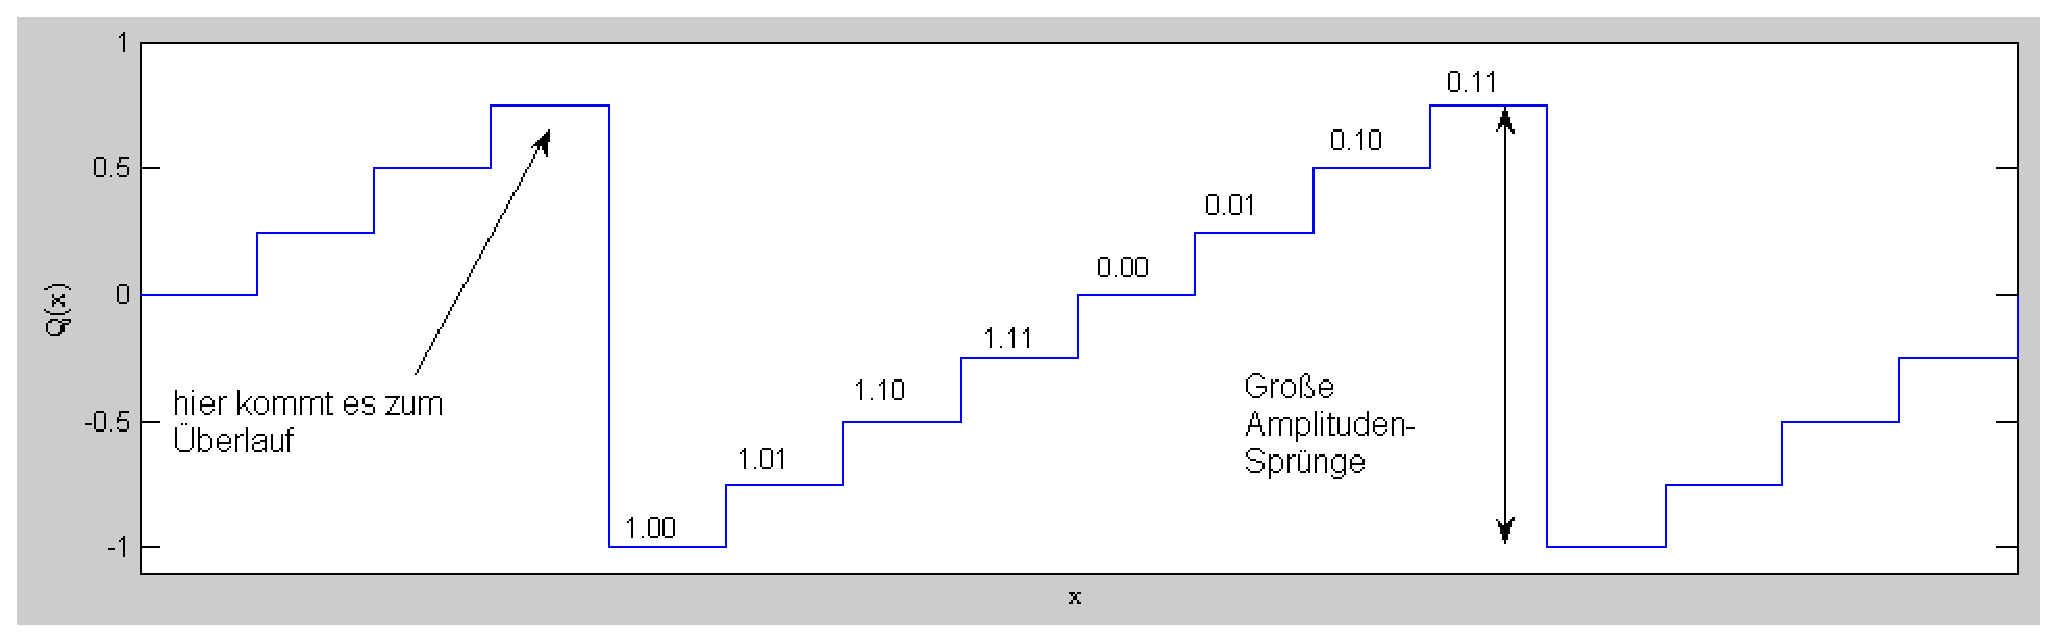
\includegraphics[width=10cm]{bilder/empfaenger/maschinenzahlen/quantisierungskennl}
	\caption{Quantisierungskennlinie mit Zweierkomplement�berlauf}
	\label{fig:quantkennl}
\end{figure}

Wie in der Abbildung sehr gut zu erkennen ist treten im Falle von �berl�ufen sehr hohe Amplitudenspr�nge auf, die zu einem stark nichtlinearem Verhalten f�hren. Allerdings ist das Modulo-2 �berlaufverhalten inh�rent und hat den Vorteil, dass Teil�berl�ufe keine Auswirkungen haben, solange das Gesamtergebniss im Bereich von [-1,1[ liegt! Ein Beispiel hierzu finden sie in Tabelle \ref{tab:teil�berl}.

\begin{table}[ht]
	\centering		
	\begin{tabular}{r|rl}
			Dezimal		& Bin�r		& \\\cmidrule{1-2}
			0.750 		& 0.110		&\\
			+0.500		& +0.100	&\\\cmidrule{1-2}
			1.250			& 1.010		&	(entspricht -0.75 $\rightarrow$ �berlauf)\\
			-0.625		& +1.011	&\\\cmidrule{1-2}	
			0.625			& 10.101	& (entspricht 0.625)\\
	\end{tabular}
	\caption{Beispiel zur Auswirkung von Teil�berl�ufen}
	\label{tab:teil�berl}
\end{table}

Vor allem bei rekursiven Systemen\footnote{Systeme mit R�ckkopplung, wie IIR-Filter (vgl. Kap.\ref{sec:digifilt})} sollte man eine Modulo-2-�berlaufkennlinie vermeiden, da durch die gro�en Amplitudenspr�nge gro�e Grenzzyklen\index{gro�e Grenzzyklen} entstehen k�nnen (vgl. Kap.\ref{subsubsec:digifilt:nonideal:koeffquant}). Zur Realisierung ist eine �berlaufbehandlung in der Arithmetikeinheit notwendig! Eine weitere M�glichkeit ist der Einsatz von Quantisierungskennlinien mit S�ttigungsverhalten\index{S�ttigungsverhalten}, wie in Abb. \ref{fig:quantkennl2} gezeigt.

\begin{figure}[ht]
	\centering 
	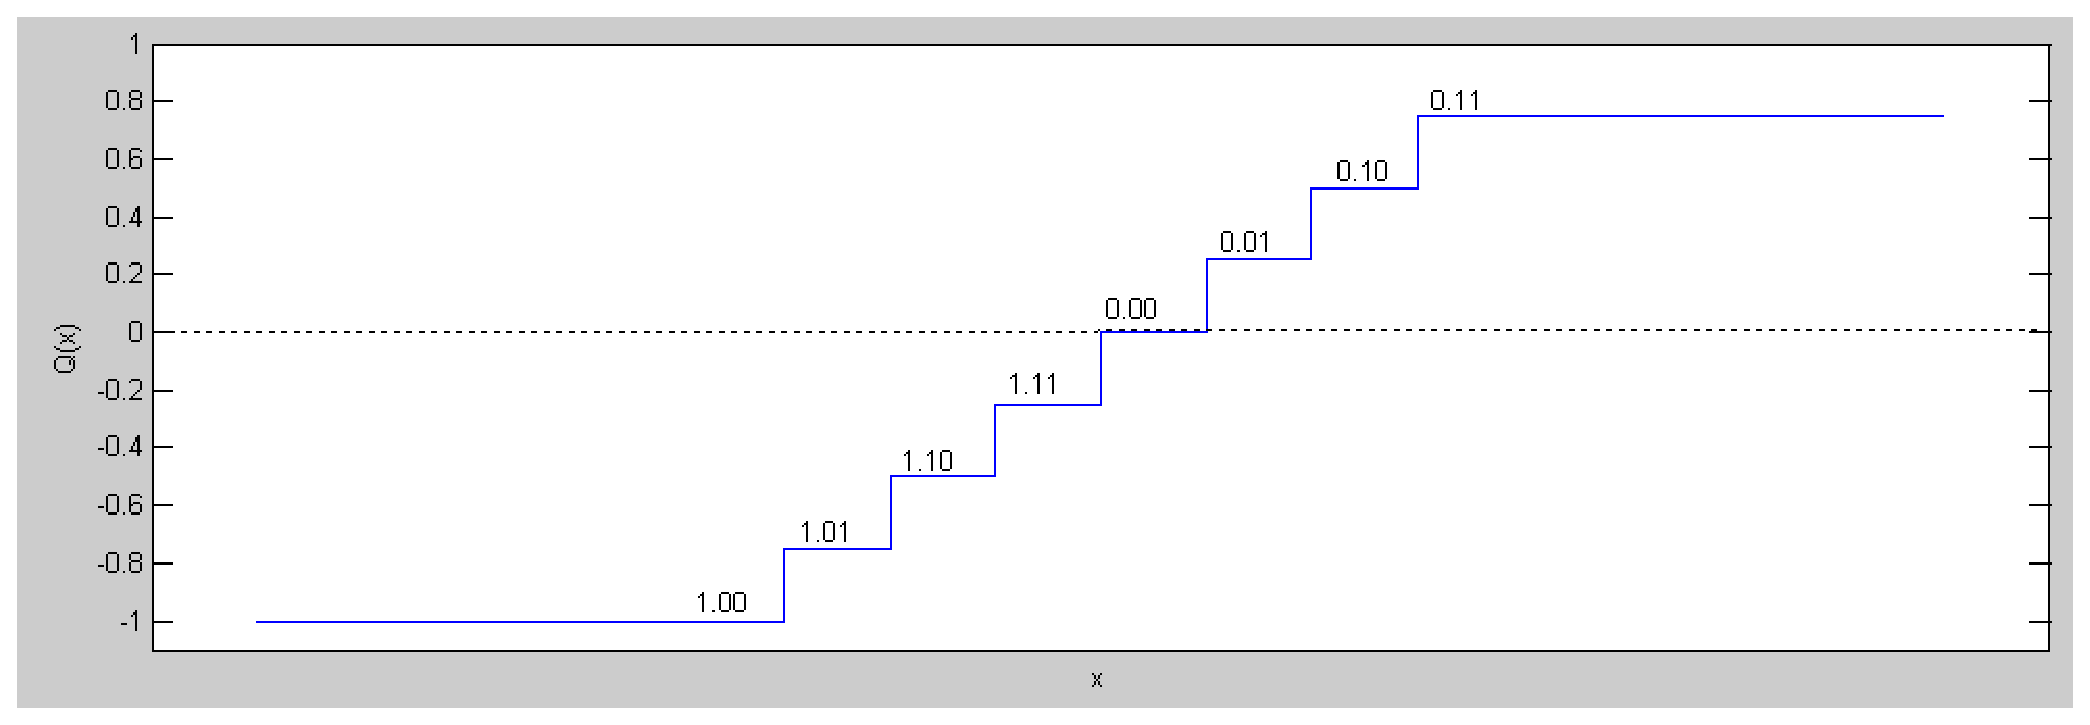
\includegraphics[width=9cm]{bilder/empfaenger/maschinenzahlen/quantisierungskennl_satt}
	\caption{Quantisierungskennlinie mit S�ttigungsverhalten}
	\label{fig:quantkennl2}
\end{figure}

\paragraph{Alignment\index{Alignment} und Sign-Extension\index{Sign-Extension}:}
Moderne DSPs besitzten eine Reihe von Registern und Speicherzellen, die unterschiedliche Wortl�ngen aufweisen. Beim Transfer von Zweierkomplementzahlen zwischen solchen Speicherpl�tzen ist zu ber�cksichtigen, wie ein Datenwort kleiner Wortl�nge in einem Speicherplatz gro�er Wortl�nge abgelegt wird.
\begin{itemize}
	\item Beim Left-Alignment\index{Left-Alignment} (``Linksb�ndiges'' Einf�gen in das Register) werden die niederwertigen Bits mit Nullen aufgef�llt,
	\item Beim Right-Alignment\index{Right-Alignment} (``Rechtsb�ndiges'' Einf�gen in das Register) ist eine Sign-Extension notwendig. Bei negativen Zahlen werden daher die h�herwertigen Bits mit Einsen aufgef�llt, bei positiven Zahlen mit Nullen. 
\end{itemize}
	
\medskip Bei der Multiplikation von Zweierkomplementzahlen sind ebenfalls Besonderheiten zu beachten. Hier unterscheidet sich die Wortl�nge des Produkts von jener der beiden Operanden. Wird eine Zahl mit $N_1$ Bits mit einer Zahl mit $N_2$ Bits multipliziert, so hat das Produkt $N_1+N_2-1$ Bits.

\begin{equation}
	N_1\cdot N_2 \Leftrightarrow N_1+N_2-1
\end{equation}


\textbf{Beispiel}\\
Betrachten wird das Produkt zweier 32-Bit-Zahlen. Das Ergebnis hat nach obiger Formel 63 Bit. Je nachdem, ob das Ergebnis Left- oder Right-Aligned in einem 64-Bit-Register abgespeichert wird erh�lt man ein zus�tzliches (redundantes) LSB oder MSB.

Aus diesem Grund wird bei einigen DSPs zwischen der Multiplikation von Integer-Zahlen (32.0) und Fractional-Zahlen (1.31) unterschieden. Bei Fractional-Zahlen muss das Ergebnis left-aligned, bei Integer-Zahlen right-aligned im Register gespeichert werden. 

\medskip Allgemein gilt, dass die Multiplikation einer Zahl im $I_1.Q_1$-Format mit einer Zahl im $I_2.Q_2$-Format ein Ergebnis im $(I_1+I_2-1).(Q_1+Q_2)$-Format ergibt.

\begin{equation}
	(I_1.Q_1)\cdot (I_2.Q_2) \Leftrightarrow (I_1+I_2-1).(Q_1+Q_2)
\end{equation}

%
\subsubsection{Zahlendarstellung im Gleitkommaformat}\label{subsubsec:siggen:representation:float}
%

Die Darstellung im Gleitkomma- oder Floating-Point-Format ist eine exponentielle Darstellung der Zahlen. Diese ist unerl�sslich zur rechnerinternen Verarbeitung sehr gro�er Zahlen, ebenso bei Anwendungen, die eine extrem hohe Genauigkeit erfordern. Im Gegensatz zur wissenschaftlichen Zahlennotation, die ja mit der Basis Zehn arbeitet, verwendet das Gleitkommaformat Zweierpotenzen. 

\medskip Eine Gleitkommazahl ist ganz allgemein aus drei Teilen aufgebaut:
\begin{itemize}
	\item Einem Vorzeichenbit \index{Vorzeichenbit} (S)
	\item der Mantisse\index{Mantisse} (M) und
	\item dem Exponenten\index{Exponent} (E).
\end{itemize}

\begin{equation}
	x=(-1)^S\cdot 2^E\cdot M
\end{equation}

Leider gibt es im Gegensatz zu Festkommasignalprozessoren, die einheitlich die Zweierkomplementdarstellung verwenden, noch kein einheitliches Zahlenformat bei Gleit\-kom\-ma-Si\-gnal\-pro\-zes\-soren. Zwar verwendet die Mehrheit das genormte 32-Bit-IEEE-Format, aber es gibt immer noch einige Hersteller, die ihre eigenen Standarts bevorzugen. 

\paragraph{IEEE-Standard P754:}\index{IEEE-Standard P754}
Dieser Standard wird - wie oben schon erw�hnt - in vielen Signalprozessoren verwendet. Man unterscheidet hier nochmals zwischen zwei unterschiedlichen Genauigkeitsstufen: Single-Precision\index{Single-Precision} und Double-Precision\index{Double-Precision}.
\begin{itemize}
	\item Single-Precision
		\begin{itemize}
			\item kleinstes Format mit 32 Bit
			\item Die Zahl wird mit 1 Vorzeichenbit, 8 Exponentenbits und 23 Bits f�r die Mantisse dargestellt
		\end{itemize}
	\item Double-Precision
		\begin{itemize}
			\item 64 Bit Genauigkeit
			\item Die Zahl wird mit 1 Vorzeichenbit, 11 Exponentenbits und 52 Bits f�r die Mantisse dargestellt
		\end{itemize}
\end{itemize}

Die Darstellung ist in der Regel so skaliert, dass die h�chstwertige Stelle der Mantisse 1 ist und daher weggelassen werden kann. In diesem Fall spricht man von der \textit{normalisierten Form}. 

Bei der Berechnung des Exponenten wird dessen Vorzeichen durch einen Offset (OS) ber�cksichtigt. Dieser betr�gt bei Single-Precision 127, bei Double-Precision 1023.

\begin{equation}
	x=(-1)^S\cdot 2^{E-OS}\cdot (1+M_f)
\end{equation}

\paragraph{Vorteile des Gleitkommaformates:}
Mit dem Floating-Point-Format kann ein sehr gro�er Zahlenbereich abgedeckt werden (Im Single-Precision-FP-Format kann beispielsweise ein Zahlenbereich von $-1.7\cdot 10^{38} ... +1.7 \cdot 10^{38}$ dargestellt werden. Au�erdem lassen sich betragsm��ig kleine Zahlen sehr viel pr�ziser darstellen als Festkomma-Zahlen (Die betragsm��ig kleinste 32-Bit-Fractional-Zahl ist $4.7 \cdot 10^{-10}$, beim single-precision Fractional-Format $1.5 \cdot 10^{-39}$).

Man kann aus den Zahlenbeispielen deutlich erkennen, dass 32-Bit-Gleit\-komma-Pro\-zess\-oren einen betr�chtlich gr��eren Dynamikbereich besitzen, als die �blichen 16- oder 24-Bit-Fest\-komma-Pro\-zess\-oren. Daher kann man sie als nahezu �berlauffrei betrachten. Ihr Nachteil liegt daf�r im deutlich komplizierteren Rechenwerk, was sich in der gr��eren Chipfl�che, einem h�heren Stromverbrauch und im h�heren Preis des Prozessors niederschl�gt.

\paragraph{Beurteilungskriterien der Eigenschaften eines Zahlenformats:}
Im letzten Abschnitt wurden die beiden Kriterien Dynamik und Pr�zision herangezogen, um die Zahlenformate zu bewerten. Diese sollen nun noch einmal kurz erl�utert werden:
\begin{itemize}
	\item Die Dynamik\index{Dynamik} beschreibt das Verh�ltnis von gr��ter und kleinster darstellbarer positiver Zahl,
	\item die Pr�zission\index{Pr�zision} den maximalen Quantisierungsfehler beim Runden.
\end{itemize}


\subsection{VHDL: Realisierung}\label{subsec:siggen:realisation}

Im Folgenden soll der CORDIC-Algorithmus in VHDL implementiert werden.

\subsubsection{VHDL-Basics: Fixed-Point Arithmetik}\label{subsubsec:vhdlbasics:fixedpoint}

\develnote{Floating-Point Arithmetik beschreiben}

F�r den CORDIC ist es notwendig, eine Look-Up-Table zu erzeugen, aus der der Algorithmus die vorberechneten Werte extrahieren kann. Problematisch f�r eine Hardwarerealisierung des CORDIC ist die Verwendung von rationalen bzw. reellen Zahlen. Eine M�glichkeit besteht darin, die math\_real-Library zu verwenden. Diese erfordert jedoch eine sehr komplexe Hardware und ist nur in F�llen anzuraten, wenn kein Weg daran vorbei f�hrt oder die Gr��e und der Leistungsverbrauch eine sehr untergeordnete Rolle spielen. Die Entwicklungsumgebung von ispLEVER unterst�tzt diese Library lediglich zur Synthesezeit. Das bedeutet, dass Berechnungen damit durchgef�hrt werden k�nnen, deren Ergebnis aber nach der Synthese feststehen muss. Bedenkt man den immensen Aufwand f�r eine Berechnung in Floating-Point Arithmetik, wird schnell klar, dass die Ressourcen der verwendeten Hardware unzureichend sind, wenn mehr als nur den CORDIC implementiert werden soll. Daher wird im Folgenden Fixed-Point-Arithmetik verwendet. Besonders das Problem der Quantisierung und der damit verbundenen Effekte muss genauer betrachtet werden.

Eine Fixed-Point Zahl wird durch eine Integerzahl ausgedr�ckt, indem man deren Wertebereich umdefiniert. Dies ist n�tig, da in VHDL lediglich Integer-Zahlen zur Verf�gung stehen. Im Praktikum wird vorerst haupts�chlich mit 8- und 16-Bit-Zahlen gearbeiten, deren Wertebereich sich von -128 bis 128 bzw. von -32768 bis 32767 erstreckt. Dieser Zahlenbereich ist besonders interessant, da das FPGA Multiplizierer mit den Wortbreiten 9, 18 und 36 zur Verf�gung stellt. 8 bzw 16-Bit sind optimal, da z.B. nach einer Addition die Wortbreite des Ergebnisses gr��er ist als die der Eingangswerte und somit eine Reserve vorgehalten werden muss. Dies wurde vom Hersteller dadurch bedacht, dass er die Multiplizierer ein Bit gr��er macht als n�tig und dem Designer damit Spielraum bei der Implementierung gibt. 

Der Bereich von -32768 bis 32767 wird umdefiniert zu -1 bis exclusive 1. Damit l�sst sich eine Genauigkeit von ca. $3,05 \cdot 10^{-5}$ erreichen, was ausreichend ist. In MAnchen Versuchen gen�gt sogar die Genauigkeit von 8 Bit.

Der genaue Wert der Zahl ergibt sich somit wie folgt.

\begin{equation}
	Z = -{N_{15}} + N_{14} \cdot 2^{-1} + N_{13} \cdot 2^{-2} + ... + N_{-14} \cdot 2^{-0}
\end{equation}

Mit Hilfe dieser Definition ist es m�glich, Addition, Subtraktion und Multiplikation wie gewohnt im Zweierkomplement auszuf�hren.

\subsubsection{VHDL-Basics: Konstanten}\label{subsubsec:vhdlbasics:constants}

Da sowohl f�r die DSS als auch f�r den CORDIC Look-Up-Tables ben�tigt werden, stellt sich die Frage, wie die vorausberechneten Werte am effektivsten in das Programm einzubinden sind. Hier bietet VHDL die M�glichkeit, Konstanten zu definieren.

\begin{verbatim}
...
  constant sv_lut0 : std_logic_vector(15 downto 0) := "0101010101010101";
...
\end{verbatim}

Um Berechnungen vor der Laufzeit des Codes, also durch die Synthese durchf�hren zu lassen, gen�gt es, den gew�nschten Ausdruck hinter die Definition zu schreiben.

\begin{verbatim}
...
  constant sv_lut1 : std_logic_vector(15 downto 0) 
        := "0101010101010101" + "0000000000000101";
\end{verbatim}

Die Synthese wird diesen Ausdruck berechnen und das Ergebnis direkt der Konstanten zuweisen.

\subsubsection{VHDL-Basics: Typenkonvertierung}\label{subsubsec:vhdlbasics:typeconversion}

Eine elegantere Variante ist die Verwendung von Konvertierungsfunktionen.

\begin{description}
	\item[conv\_std\_logic\_vector(<VALUE>, <WIDTH>)] Konvertiert eine Integerzahl \emph{VALUE} in den Typ std\_logic\_vector mit der angegeben Breite \emph{WIDTH}.
	\item[conv\_unsigned(<VALUE>, <WIDTH>)] konvertiert eine Integerzahl in eine unsigned Darstellung des Typs std\_logic\_vector.
	\item[conv\_signed(<VALUE>, <WIDTH>)] Konvertiert in eine Signed-Darstellung des std\_\-lo\-gic\_\-vec\-tor-Typs.
\end{description}

Bei conv\_std\_logic\_vector ist darauf zu achten, dass die Interpretation eingebundenen Paket (signed oder unsigned) abh�ngt.

Weitere Konvertierungsroutinen werden im Laufe des Praktikums folgen.

\subsubsection{VHDL-Basics: Mehrdimensionale Arrays}\label{subsec:vhdlbasics:array:multidim}

Bisher wurde lediglich die Festlegung der einzelnen Zeilen behandelt, allerdings ist dies f�r eine Tabelle recht ineffizient. Hierzu verwendet man ein Array des Typs std\_logic\_vector, um jede Zeile durch einen Index ansprechen zu k�nnen, wie es beispielsweise mit den einzelnen Bits des std\_logic\_vector m�glich ist. In VHDL ist es erlaubt, mehrdimensionale Arrays beliebiger Tiefe zu erzeugen. Derzeit erlaubt die Synthese aber maximal zweidimensionale Arrays.

\advise{Arrays maximal zweidimensionale in Hardware implementieren.\\ Std\_logic\_vector ist selbst ein eindimensionales Array des Typs std\_logic, daher maximal eine weitere Dimension zul�ssig}

Eine M�glichkeit eine LUT zu erzeugen s�he also wie folgt aus:

\begin{verbatim}
...
  type tva_LUT is array(0 to 1) of std_logic_vector(3 downto 0);
	
  constant my_lut : tva_LUT := (("0100"),("1000"));
...
\end{verbatim}

Der Aufbau der ben�tigten LUT erfolgt analog zum obigen Beispiel.

\subsubsection{VHDL-Basics: Zahlentypen}\label{subsubsec:vhdlbasics:numbertypes}

Eine Darstellung von Zahlen erfolgt in Hardware �blicherweise mittels mehrerer einzelner Signale in bin�rer Form z.B. mittels des Zweierkomplements. Programmieren w�re jedoch mit dieser Methode recht umst�ndlich und die �bersetzung k�nnte auch gut die Synthese erledigen. Dazu werden an dieser Stelle einige neue Datentypen vorrgestellt:

\begin{description}
	\item[integer] �bersetzt in 32-bit, Werte zwischen $-2^{31} \textnormal{ und } 2^{31}-1$
	\item[natural] �bersetzt in 31-bit, Werte zwischen $0 \textnormal{ und } 2^{31}-1$ (Vorsicht!!! nicht 32-bit)
	\item[positive] �bersetzt in 31-bit, Werte zwischen $1 \textnormal{ und } 2^{31}-1$ (Vorsicht!!! auch nur 31-bit)
\end{description}

Jeden der oben genannten Zahlentypen kann man mit \emph{range <FROM> to <TO>} eingrenzen und so die Synthese anweisen, die minimale Anzahl an Signalen zu verwenden. Bei der Deklaration w�rde dies wie folgt aussehen:

\begin{verbatim}
...
  signal si_counter : integer range 0 to 40;
...
\end{verbatim}

Dies w�rde die Synthese veranlassen, intern einen 6-Bit-Vektor ($0 \textnormal{ bis } 2^{6}-1=63$) zu verwenden.

%\advise{Falls man einen eingeschr�nkten Datentyp in einer Abfrage verwendet, der nicht exakt mit $0 \textnormal{ bis } 2^{n}-1$ abgebildet werden kann, so ist hier in jedem Fall ein  einzuf�gen, selbst wenn man auf alle erlaubten Werte der Range pr�ft, da sonst die �brigen Werte bis $2^{n}-1 \textnormal{ bzw. } 0$ bis zum Anfangswert der Range nicht ber�cksichtigt werden und dies zur Verwendung von Latches f�hrt.}

\subsubsection{VHDL-Basics: Records}\label{subsubsec:vhdlbasics:records}

�hnlich wie in Software-Programmiersprachen k�nnen auch in VHDL verschiedene Signale zu einem Record geb�ndelt werden, um auf diese als Ganzes zugreifen zu k�nnen. Ein Record wird �ber einen eigenen Typ definiert.

\develnote{Zugriff auf Record beschrieben}

\begin{verbatim}
...
  type <REC_NAME> is 
    record
      DAY: positive range 1 to 31;
      MONTH : positive range 1 to 12;
      YEAR : integer;
    end record;
...
\end{verbatim}

\subsubsection{VHDL-Basics: Komponenten}\label{subsubsec:vhdlbasics:components}

Bisher wurde Ihnen die Erstellung eigener Module abgenommen. Bei gr��eren Modulen empfiehlt es sich aus Gr�nden der �bersichtlichkeit, dieses in mehrere Untermodule aufzugliedern. VHDL erm�glicht dies, indem man Komponenten erst deklariert und anschlie�end instantiiert. Die Instantiierung ist n�tig, da man dadurch ein Modul mit unterschiedlichen Parametern (Generics, Port-Mapping) mehrmals in einem File verwenden kann, �hnlich den Klassen einer objektorientierten Programmiersprache. Eine Komponente deklariert man wie folgt:

\begin{verbatim}
...
architecture ...
...
  component <COMP_NAME>
  	[generic(
  		<GEN_NAME> : <TYPE> [:= <VALUE>] [;
  		<GEN_NAME> : <TYPE> [:= <VALUE>]; ...]
  	);]
    port(
      <PORT_NAME> : <DIR> <TYPE> [;
      <PORT_NAME> : <DIR> <TYPE>; ...]
    );
  end component;
...
begin
...  
\end{verbatim}

\advise{Es ist ratsam in eigenen Modulen, f�r Ports lediglich std\_logic und std\_logic\_vector zu verwenden, da dies der Hardware am n�chsten kommt und bei der Synthese sonst oftmals Schwierigkeiten auftreten, �ber Modulgrenzen hinweg zu optimieren. F�r Generics hingegen d�rfen nur Integer-Typen (Interger, Boolean, Natural und Positive) verwendet werden.}

Hat man die Komponente in seinem Code deklariert, erfolgt die Instantiierung:

\begin{verbatim}
... 
architecture ...
...
begin
...
  <INSTANT_NAME>: <COMP_NAME>
    [generic map (
      <GEN_NAME> => <CONST_NAME> [;
      <GEN_NAME> => <CONST_NAME>; ...]
    );]
    port map (
    	<PORT_NAME> => <SIGNAL_NAME> [;
    	<PORT_NAME> => <SIGNAL_NAME>; ...]
    );
...
\end{verbatim}

\ifthenelse{\xemacs}{%
Bei Verwendung von XEmacs, wird einem diese aufwendige Tipparbeit nat�rlich erspart, indem man wieder auf die n�tzlichen Funktionen, die �ber die rechte Maustaste verf�gbar sind, zur�ck greift. Dazu wie gewohnt, in den Quellcode der Komponente gehen, den Port mittels \emph{Port$\rightarrow$Copy} in den Template-Buffer von XEmacs bef�rdern, in den eigenen Quellcode zur�ckgehen und dort einerseits im Deklarationsteil der architecture mittels \emph{Port$\rightarrow$Paste as Component} die Komponente einf�gen und mittels \emph{Port$\rightarrow$Paste as Instance} im Code-Teil der architecture die Instantiierung. Nun ggf. noch das Mapping auf die gew�nschten Signalnamen und Konstanten korrigieren, fertig.
}{} % Tja, Nicht-XEmacser ist nicht zu helfen.

\subsubsection{VHDL-Basics: Multiplizierer}\label{subsubsec:vhdlbasics:multiplier}

In dem verwendeten FPGA sind fertige Multiplizierer bereits integriert. Diese k�nnen auf unterschiedliche Art und Weise verwendet werden. Einerseits bietet ispLEVER mit dem Programmmodul IPexpress, mit dem man Module generieren und diese dann in den eigenen Code als Komponente einbinden kann. Oft sind die von IPexpress generierten Module optimiert und bieten manche Features, auf die man sonst keinen Zugriff erlangt. Allerdings kann man ebenso das Synthesetool zur Optimierung nutzen und nach dem Syntheselauf anhand der Ausgaben, die jene erzeugt, entscheiden, ob man mit dem Ergebnis zufrieden ist, oder ob man doch auf IPexpress zur�ckgreift. In der Ausgabe finden sich zwei Bereiche, aus denen die Verwendung der DSP-Einheiten hervorgeht. Einmal in Form einer Matrix, die die Verwendung der einzelnen Multiplizierer der DSP-Bl�cke angibt und zum anderen eine Information �ber die Konfiguration der DSP-Bl�cke (MULTADDSUM, MAC,...).

Der Einfachheit wegen wird im Rahmen des Praktikums auf IPExpress verzichtet, der Multiplizier-Operator in VHDL verwendet und die Synthese �bernimmt die Arbeit.

\begin{verbatim}
...
  sv_mult_result <= sv_var_a * sv_var_b; -- std_logic_vector
  si_mult_result <= si_var_a * si_var_b; -- integer
...
\end{verbatim}

Die Synthese erkennet bei diesem Beschreibung selbstst�ndig, ob ein 9-, ein 18- oder ein 36-Bit-Multiplizierer n�tig ist. Diese Arten von Multiplizierern stellt der verwendete FPGA zur Verf�gung.

\advise{Da die Anzahl der kleineren 9-Bit-Multiplizierer gr��er ist als die der 18- bzw. 36-Bit-Multiplizierer, ist es hier besonders wichtig, den Wertebereich der Signale so klein wie m�glich zu halten. Daher sollten die Interger-Typen bei der Deklaration unbedingt einen m�glichst kleinen Wertebereich zugewiesen bekommen.}

\subsection{VHDL: Beschreibung CORDIC-Base}\label{subsec:siggen:vhdl:cordic:base}

\paragraph{Aufgabe 1: Look-Up Table}

Erstellen Sie in \verb|03_Siggen\cordic_lut.vhd| eine Look-Up Table, die alle ben�tigten Informationen f�r einen 10-stufigen CORDIC-Algorithmus beinhaltet. Diese soll in Form eines Moduls aufgebaut sein und als Schnittstelle die Ports aus Tabelle \ref{tab:LUT-Ports} besitzen. 

Die Werte der LUT kann man entweder durch festes Kodieren der Zahlen oder durch Berechnen w�hrend der Synthese mittels des Packages ieee.math\_real einf�gen. Wer schon ein wenig mehr Erfahrung in VHDL hat, kann dies gerne versuchen, er gen�gt jedoch, die Werte mit dem Taschenrechner zu berechnen und in den Quellcode einzutippen. Ein Beispiel, f�r die elegante Methode ist im VHDL-Code des DDS-Moduls zu finden.

\advise{Verwenden sie ausschlie�lich Integer-Typen bzw. std\_\-lo\-gic\_\-vec\-tor zur Darstellung von Zahlen. Diese k�nnen als Einzige von der Synthese in Hardware umgesetzt werden. F�r die Synthese existieren keine Fixed-Point Zahlen.}

\begin{table}
	\centering		
	\begin{tabular}{|c|c|c|l|}\hline
		\textbf{Portname} & \textbf{Direction} & \textbf{Bits} & \textbf{Beschreibung} \\\hline
	  STEPS & In & 4 & Die Anzahl der Schritte des Algorithmus \\
	  ALPHA\_I & Out & 16 & Der Drehwinkel  \\
	  TAN\_ALPHA\_I & Out & 16 & Der Tangens des Drehwinkels \\
	  K\_I & Out & 16 & Der Skalierungsfaktor f�r diesen Schritt \\
	  K\_G & Out & 16 & Der Gesamtskalierungsfaktor f�r diesen Schritt \\\hline
	\end{tabular}
	\caption{Port des LUT-Moduls}
	\label{tab:LUT-Ports}
\end{table}

\subparagraph{Hinweis}

Eine LUT kann �blicherweise mittels eines Arrays aufgebaut werden. Versuchen Sie, die gestellte Aufgabe m�glichst elegant zu l�sen und bedenken Sie, dass die vorangegangen Grundlagen bei der L�sung des Problems n�tzlich sein k�nnen.

\paragraph{Aufgabe 2.1: CORDIC-Basis-Algorithmus}

Programmieren Sie nun den CORDIC-Basis-Algorithmus, der es erm�glicht, einen beliebigen Vektor um $\pm100^{\circ}$ zu drehen. Binden Sie dazu das in der letzten Aufgabe erstellte Modul cordic\_lut.vhd ein. Der vorgefertigte Quellcode cordic\_base.vhd mit den Ports und Generics existiert bereits in ihrem Paraktikumsverzeichnis. Die architecture ist von Ihnen zu programmieren. Die Anzahl der Stufen soll �ber das Generic \emph{STEPS} von 1 bis 10 gesteuert werden k�nnen.

\textbf{Hinweis:} Verwenden Sie einen Z�hler, der durch die einzelnen Iterationsstufen z�hlt und die Hardware steuert.

\subsection{MODELSIM: Simulation CORDIC-Base}\label{subsec:siggen:sim:cordic}

\paragraph{Aufgabe 2.2: CORDIC-Basis-Algorithmus}

Simulieren sie das fertige Modul und verifizieren sie dessen Fehlerfreiheit. Verwenden sie dazu die Testbench cordic\_base.vhd. Drucken Sie die Waveform aus Modelsim aus und f�gen sie diese ihrem L�sungsordner bei.


\subsection{VHDL: Beschreibung 360�-CORDIC}\label{subsec:siggen:cordic:full}

\paragraph{Aufgabe 3.1: 360\textdegree-CORDIC-Algorithmus}

Entwerfen Sie ein Modul, dass den CORDIC aus Aufgabe 2 einbindet und auf Drehwinkel von 360\textdegree erweitert. Verwenden Sie das File \verb|cordic_full.vhd|, binden sie \verb|cordic_base.vhd| ein und erweitern es um die geforderte Funktionalit�t.

\subsection{MODELSIM: Simulation 360�-CORDIC}\label{subsec:siggen:sim:cordic:full}

\paragraph{Aufgabe 3.2: 360\textdegree-CORDIC-Algorithmus}

Simulieren Sie den Code ebenfalls und drucken Sie auch diese Waveform aus.

\subsection{VHDL: Tonerzeugung}\label{subsec:siggen:vhdl:soundgen}

\paragraph{Aufgabe 4.1: Der erste eigene Ton}

Vervollst�ndigen Sie das Modul \verb|siggen.vhd| so, dass ein Ton mit ca. 9 kHz erzeugt wird. Verwenden Sie den berechneten Vektor als Eingabevektor f�r den n�chsten CORDIC-Durchlauf.

Wie lautet die Formel zur Berechnung der Ausgangsfrequenz des CORDIC-Si\-gnal\-ge\-ne\-ra\-tors?
\answergame{5}{
	\begin{math}
		f_{out} = \frac{f_{clk}}{\textnormal{STEPS}} \cdot \frac{\Theta}{360^{\circ}}
	\end{math}
}

\subsection{MODELSIM: Tonerzeugung}\label{subsec:siggen:sim:soundgen}

\paragraph{Aufgabe 4.2: Der erste eigene Ton}

Simulieren Sie \verb|tone\_gen.vhd| mit der vorgefertigen Testbench \verb|siggen\_tb.vhd| �ber einen ausreichend langen Zeitraum (ca. 1000 Perioden). Was stellen Sie fest?

\answergame{3}{Die Amplitude �ndert sich (steigt stetig an/f�llt stetig ab, je nach Rundung des Korrekturfaktors)}

Worauf ist dieses Verhalten zur�ckzuf�hren?

\answergame{4}{Durch die Fixed-Point-Arithmetik kommt es zu Rundungsfehlern beim Korrekturfaktor. Die Amplitude verf�lscht sich bei jeder Iteration.}

\paragraph{Aufgabe 5.1: Verbesserung des COR\-DIC-Si\-gnal\-ge\-ne\-ra\-tors}

Wie ist\\ \verb|tone\_gen.vhd| zu ver�ndern, um diesen Fehler zu beseitigen?

\answergame{3}{Fester Eingangsvektor; Ver�nderung/Aufsummiern des Drehwinkels Theta bei jedem CORDIC-Durchlauf. Wenn gr��er 360�, dann wieder bei 0 beginnen.}

Welche M�glichkeit zur Hardware-Einsparung ergibt sich durch diese Ver�nderung noch?

\answergame{3}{Der Korrekturfaktor kann schon vorher in den Eingangsvektor eingerechnet werden und der Multiplizierer am Ausgang entf�llt}

\paragraph{Aufgabe 5.2: Simulation der Vebesserungen}

Simulieren Sie den verbesserten Signalgenerator.

\subsection{TEST: Praxis}\label{subsec:siggen:test}

\subparagraph{Aufgabe 6}

Testen Sie Ihren Signalgenerator mit Hilfe der Hardware.


	\section{Versuch 4: Pegelanzeige}\label{sec:level}
  \develnote{Hier programmieren wir eine Pegelanzeige. Evtl. wird diese auch vorgegeben!? Wir werden sehen}

\subsection{Konzept}\label{subsec:level:idea}

Da die Pegel am Mikrofoneingang stark schwanken, ist es w�nschenswert, die Verst�rkung nachzuf�hren, um eine maximale Aussteuerung der AD-Wandler zu erhalten. Ebenso ist es n�tzlich, die Pegel am Ausgang des sp�ter verwendeten Filters anzeigen zu k�nnen. Da die Funktion einer Pegelanzeige am Einfachsten mit dem Ausgang des Signalgenerators verifiziert werden kann, wird dieser Block an diese Stelle vorgezogen.

\subsection{Realisierungsm�glichkeiten}\label{subsec:level:possibilities}

Da Pegel leistungsbezogene Angaben sind, muss eine quadratische Mittelwertbildung �ber die Amplitude der Spannung durchgef�hrt werden. Die Leistung eines Signals ist definiert durch:

\begin{equation}
	\bar{P} = frac{1}{t_M} \cdot \int\limits_{t}^{t+t_M} \left|U^2\right| \cdot dt = frac{1}{t_M} \cdot \int\limits_{t}^{t+t_M} U^2 \cdot dt
\end{equation}

Um eine richtige Anzeige zu erhalten, muss eine Mittelung �ber einen relativ langen Zeitraum $t_M$ erfolgen. Dieser sollte zwischen 50 und 100 ms betragen, um noch synchron zum Geh�rten zu wirken.

\subsubsection{Pegeldefinition}\label{subsubsec:level:definition}

Pegel werden meist in dBm angegeben. Der die Spannung bei einem Pegel von 3dBm betr�gt $\approx0,31 V_{eff}$. 

Auf eine Simulation in MATLAB kann hier aufgrund der Einfachheit verzichtet werden.

\subsection{VHDL: Realisierung}\label{subsec:level:realization}

\subsubsection{VHDL-Basics: Variablen}

Bisher wurde die M�glichkeit gezeigt, Werte in Signalen zu speichern. Besitzt eine Architecture hingegen mehrere Prozesse, wird dies schnell un�bersichtlich. 

In Prozessen darf man sogenannte Variablen deklarieren, die lediglich lokale G�ltigkeit besitzen. Im Vergleich zu Signalen ergeben sich jedoch erhebliche Unterschiede, die selbst f�r erfahrene Programmierer eine Fehlerquelle darstellen.

Der syntaktische Teil, die Deklaration, ist folgenderma�en aufgebaut.

\begin{verbatim}
<PROCNAME>: process (<SENSITIVITY LIST>)
  variable <VARNAME>: <TYPE>[ := <INITIALIZATION>];
  ...
begin
  ...
end process <PROCNAME>;
\end{verbatim}

Variablen haben, wie bereits erw�hnt, nur lokale G�ltigkeit. Dies schl�gt sich auch in einer schlechten Zug�nglichkeit w�hrend der Simulation nieder. Auch �ndert sich die Syntax der Wertzuweisung. Signalen wird mittels \verb|<=| ein Wert zugewiesen, Variablen hingegen mittels \verb|:=|. Ein Beispiel hierzu:

\begin{verbatim}
sig_1 <= sig_2;
sig_2 <= var_1;
var_1 := var_2;
var_2 := sig_2;
\end{verbatim}

Ein grundlegender Unterschied zwischen Siganlen und Variablen ist, dass Signale bis zum n�chsten Ereignis ihren Wert behalten, egal in welcher Reihenfolge im Code sie stehen, Variablen hingegen sofort den zugewiesenen Wert erhalten.

Folgendes Beispiel soll dies verdeutlichen:

\begin{verbatim}
var_1 := var_1 + 5;
var_2 := var_1 + 5;

sig_1 := sig_1 + 5;
sig_2 := sig_1 + 5;
\end{verbatim}

Hier erh�lt \verb|var_2| sofort den Wert von \verb|var_1 + 10|, w�hrend \verb|sig_2| den Wert von \verb|sig_1 + 5| erst beim n�chsten Ereignis erh�lt.

Eine Variable in dieser Verwendung stellt ein erhebliches Problem f�r die Synthese dar und kann diese trotz der Einfachheit der Anweisung sehr komplexen Code erzeugen. Im einfachsten Fall wird Hardware doppelt erzeugt, um die Berechnung vorwegzunehmen. Auch die Geschwindigkeit kann sich erheblich reduzieren. 

\advise{Reihenfolge der Zuweisung von Variablen beachten, sonst kann es zu unerwartetem Verhalten f�hren.}

Beachtet man bestimmte Regeln, so treten wenig Probleme bei der Verwendung von Variablen auf. Die wichtigste Regel bei Variablen besteht darin, die Zuweisung der Variablen an das Ende des Prozesses zu verlegen, wenn man nicht ausdr�cklich plant, das spezielle Verhalten der Variablen zu nutzen um den Code zu verschlanken.

In Software-Programmiersprachen wird davon abgeraten, globale Variablen (bei VHDL  vergleichbar mit Signalen) zu verwenden. In VHDL gestaltet sich dies ein wenig anders. Hier wird unerfahrenen Programmierern geraten, nur Signale zu verwenden. Bei �berschaubaren Prozessen von wenigen Zeilen ist es jedoch ratsam, auf Variablen zur�ckzugreifen, um den Aufwand an Signaldeklarationen im Deklarationsteil so gering wie m�glich zu halten.

Ein weiterer Grund f�r die Verwendung von Variablen ist, dass oft tempor�re Signale in vielen Prozessen gleiche Namen tragen, allerdings nicht den gleichen Wert besitzen. Einigt man sich hier auf gleiche Namen, so wird das Verst�ndnis des Codes erleichtert, da man sich an bekannten Strukturen orientieren kann. Ein Beispiel ist die Flankenerkennung von Signalen. Hierzu ben�tigt man ein tempor�res Signal (respektive Variable), die den Wert des Signals des letzten Taktzyklusses speichert, um im N�chsten diesen mit dem aktuellen vergleichen zu k�nnen. Hier bietet sich beispielsweise der Variablenname vl\_edge\_detect an. So sp�ter zu jeder Zeit bekannt, dass es sich hier um die Flankenerkennung handelt.

\subsubsection[VHDL-Basics: Simulation <-> Synthese]{VHDL-Basics: Unterscheidung Simulation <-> Synthese}

In Modelsim lassen sich keine Variablen auslesen. Es ist daher unumg�nglich, f�r das Debugging ein Signal zu verwenden. In Handware darf dieses nicht implementiert werden, und die Synthese ist anzuweisen, dieses zu ignorierenIn VHDL geschieht dies durch folgende Schl�sselworte:

\begin{verbatim}
--synopsis translate_off
...
--synopsis translate_on
\end{verbatim}

Die Anweisungen an Stelle des Platzhalters werden von der Synthese ausgenommen. Somit wird es m�glich, Signale und deren Zuweisungen lediglich in der Simulation zu erlauben.

Auch andere Anwendungen existieren, die auf solche Anweisungen angewiesen sind. Beispielsweise die Modelle f�r die Multiplizierer die in IPExpress generiert wurden. Die Synthese verwendet dann die DSP-Bl�cke, die in der Hardware verf�gbar sind.

\subsection{VHDL: Beschreibung der Hardware}\label{subsec:level:HWdesc}

Die Pegelanzeige soll Pegel in Abstufungen von 3 dB anzeigen, wobei die rote LED ab einem Pegel von $+1,5 dBm$ leuchten soll, die obere gelbe ab einem Pegel von $-1,5 dBm$, die zweite gelbe ab $-4,5 dBm$, usw.

\paragraph{Aufgabe 1.1:}

Realisieren sie in VHDL die Pegelanzeige in der Datei \\ \verb|04_Levelmeter\levelmeter.vhd|.

\subsection{MODELSIM: Simulation der Beschreibung}\label{subsec:level:sim}

\paragraph{Aufgabe 1.2:}

Simulieren sie die zuvor programmierte Pegelanzeige. Erstellen sie hierzu Ihre eigene Testbench mit geeigneten Stimuli. Orientieren sie sich an den bereits verwendeten Testbenches.

\subsection{TEST: Praxis}\label{subsec:level:test}

\paragraph{Aufgabe 2:}

Verkn�pfen sie nun den Eingang der Pegelanzeige mit dem von AD-Wandler kommenden Mikrofonsignal und testen sie die Anzeige in der Realit�t. Alternativ schlie�en sie den Line-In-Eingang an den PC an und spielen mit Winamp ein kurzes Musikst�ck ab.
	\section{Versuch 5: Modulator}\label{sec:modulator}
	\develnote{Wieder ein einfacher Multiplexer, diesmal lassen wir allerdings die gesamte entity und architecture programmieren. Die Studies sollen ja schlie�lich VHDL lernen. Auch in MATLAB werden jetzt keine Strukturen mehr vorgegeben. Die Studenten sollen jetzt ihre Skripten / Funktionen selbst erstellen.}

\subsection{Konzept}\label{subsec:modulator:concept}

Die �bertragung von Daten �ber eine beliebige �bertragungsstrecke ist nicht ohne weiteres (fehlerfrei) m�glich. W�rde man die Daten 1:1 �ber den Kanal schicken, das hei�t zum Beispiel durch Codierung der Null-Bits mit einer Spannung von 0 Volt und der Eins-Bits mit 3.3 Volt, w�re das Ergebnis ziemlich ern�chternd. Kleinere Spannungsschwankungen wirken sich in diesem Fall direkt auf das Empfangssignal aus. Um hier Fehler schon im Vorfeld auszuschlie�en wird das Signal vor der �bertragung moduliert, wodurch die St�ranf�lligkeit verringert wird.

\subsection{Realisierungsm�glichkeiten}\label{subsec:modulator:possibilities}

Um das Praktikum nicht zu kompliziert zu gestalten werden wir uns mit einer einfachen FSK-Modulation\footnote{Frequency Shift Keying}\index{FSK-Modulation} begn�gen. Hierbei werden Nullen und Eisen durch zwei Sinusschwingungen unterschiedlicher Frequenz dargestellt. F�r eine logische Null wird die eine, f�r eine Eins die andere Frequenz �bertragen. Sie haben im Verlauf der ersten Kapitel die n�tigen Baugruppen bereits kennengelernt. Nun werden sie den kompletten FSK-Sender, wie im Blockschaltbild in Abb. \ref{abb:sender_blockschaltbild2}, aufbauen.

\begin{figure}[ht]
	\centering 
	%\psfrag{01}{MATLAB Workspace}
	\includegraphics[width=10cm]{bilder/sender/sender_blockschaltbild}
	\caption{Sender Blockschaltbild}
	\label{abb:sender_blockschaltbild2}\index{Sender Blockschaltbild}
\end{figure}

\subsection{MATLAB: Programmierung}\label{subsec:modulator:matlab}

\paragraph{Aufgabe 1:}
Schreiben sie ein MATLAB-Skript, das unter Verwendung der bisher programmierten Funktionen \textit{PRNseq.m}, \textit{cordic.m} und \textit{oszillator.m} die oben beschriebene Funktion erf�llt. Stellen sie die Ergebnisse graphisch dar. Legen sie alle verwendeten Skripten und die erhaltenen Ergebnisse im Verzeichnis \pathtomatlab{Sender\textbackslash Modulator} ab.

\paragraph{Aufgabe 2:}
Wie kann man die gleiche Funktion mit deutlich geringerem Hardwareaufwand realisieren? Implementieren sie ein einfacheres L�sungskonzept in MATLAB!
\answergame{4}{
Ersetzt man den Inverter und die beiden Multiplikatoren durch einen einfachen Multiplexer, der je nach Datenbit eine der beiden Frequenzen an den CORDIC-Algorithmus weiterreicht, so kommt man mit einem einzigen Sinusgenerator aus (vgl. Abbilung \ref{abb:Sinus2}). 
}
\ifthenelse{\printsolution}{
\begin{figure}[ht]
	\centering 
	%\psfrag{01}{MATLAB Workspace}
	\includegraphics[width=9cm]{bilder/sender/Sinusgenerator2}
	\caption{Vereinfachter Modulator}
	\label{abb:Sinus2}
\end{figure}
}

\subsection{VHDL: Realisierung}\label{subsec:modulator:vhdl:realisation}

\subsection{VHDL: Modulator mit zwei Signalgeneratoren}\label{subsec:modulator:vhdl:HWdesc}

Um den kompletten Modulator in Hardware aufzubauen haben Sie schon alle ben�tigten Module in den vorherigen Aufgaben erstellt. 

\paragraph{Aufgabe 1.1:} 

Setzen sie den Modulator mit Hilfe der erstellten Module in VHDL zusammen \\
(\verb|05_Modulator\stud_toplevel.vhd| Importieren sie die ben�tigten Module in das aktuelle Projekt (vgl. \ref{fig:ispLeverimportfile} und \ref{fig:ispLeverimportdialog}). Erstellen sie die Komponentendeklaration und instanziieren sie zwei Signalgeneratoren mit unterschiedlichen Parametern. Die beiden Modulationsfrequenzen, die sie verwenden sollen, erhalten Sie von Ihrem Betreuer.

\begin{figure}
	\centering
		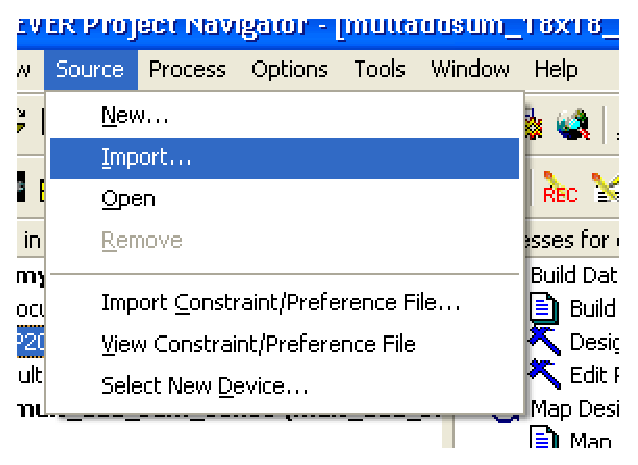
\includegraphics{bilder/sender/ispLeverimportfile.eps}
	\caption{VHDL-Datei importieren}
	\label{fig:ispLeverimportfile}
\end{figure}

\begin{figure}
	\centering
		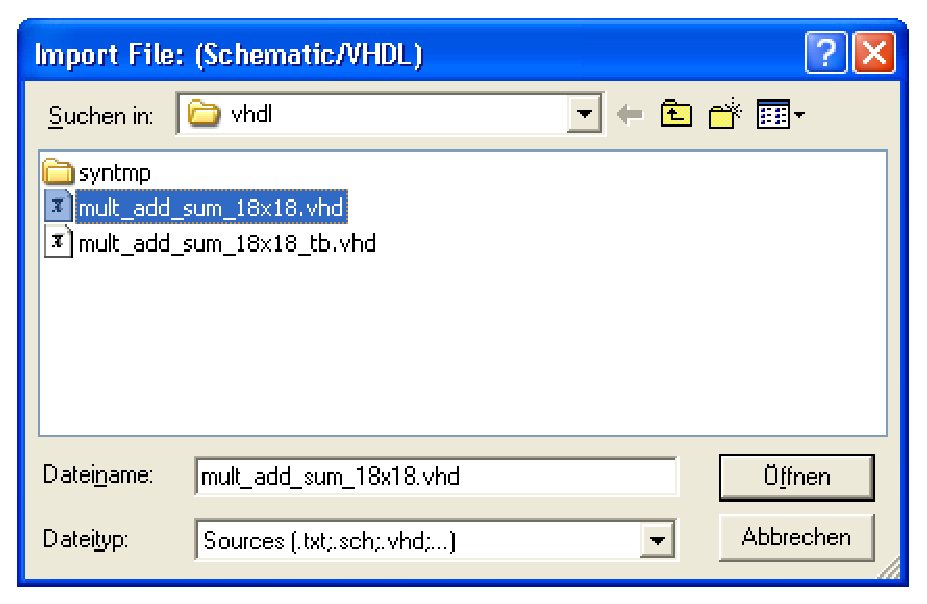
\includegraphics{bilder/sender/ispLeverimportdialog.eps}
	\caption{Importdialog}
	\label{fig:ispLeverimportdialog}
\end{figure}


\subsection[MODELSIM: Simulation mit zwei Signalgeneratoren]{MODELSIM: Simulation der Beschreibung mit zwei Signalgeneratoren}\label{subsec:modulator:sim}

\paragraph{Aufgabe 1.2:}

Simulieren Sie den zuvor erstellten Modulator mit Hilfe eines Digitalsignals, das von einem 4-Bit-PRN-Schieberegister mit XOR-Feedback �ber der letzten (MSB) Stufe \\
\verb|sv_prn_reg(3) <= sv_prn_reg(1) xor sv_prn_reg(0)|\\
erzeugt wird. Als Anfangsbelegung verwenden sie \verb|"1001"|. Der Schiebetakt soll bei etwa $1Hz$ liegen.

\paragraph{Aufgabe 2:}

Betrachten sie das modulierte Signal zu den Umschaltzeitpunkten genauer. Was stellen Sie fest?

\answergame{3}{Spr�nge im Ausgangssignal, die zu starken Oberwellen f�hren k�nnen.}

\subsection{VHDL: Modulator mit einem Signalgenerator}\label{subsec:modulator:HWdesc2}

\paragraph{Aufgabe 3:}
Verbessern Sie das Verhalten, indem Sie nur einen Signalgenerator verwenden und dessen Drehwinkel �ber einen Multiplexer ver�ndern.

\subsection[MODELSIM: Beschreibung mit einem Signalgenerator]{MODELSIM: Simulation der Beschreibung mit einem Signalgenerator}\label{subsec:modulator:sim2}

Simulieren Sie auch dies und kontrollieren nun das Verhalten im �bergangsbereich.

Was stellen sie bez�glich der Stetigkeit des Ausgangssignals fest?
\answergame{3}{Keine Spr�nge im Ausgangssignal}

Warum ist dies g�nstig f�r unsere Anwendung?
\answergame{4}{Keine Oberwellen, dadurch weniger St�rungen der Nachbarfrequenzen.}

\subsection{TEST: Praxistest}\label{subsec:modulator:test}

Testen Sie nun Ihren Entwurf auf der Hardware.

	
% Empf�nger
			
	\cleardoublepage
\chapter{Empf�nger}\label{chap:receiver}
\thispagestyle{empty}

\section{Aufbau}\label{sec:receiver:structure}

$\overline{H}$

\begin{figure}[ht]
	\centering 
%	\psfrag{06}{$N$}
	\includegraphics[width=10cm]{bilder/empfaenger/Empf�ngerstufe}
	\caption{Blockschaltbild der Empf�ngerstufe}
	\label{fig:Empf�nger}
\end{figure}

Der Empf�nger ist aus zwei identischen Zweigen aufgebaut. Jeder Zweig besteht, wie in Abb. \ref{fig:Empf�nger} dargestellt, aus einem Bandpass\index{Bandpass}, einem H�llkurvendemodulator\index{H�llkurvendemodulator} und einem Tiefpass\index{Tiefpass}. Am Eingang wird das FSK-modulierte Signal (vgl. Abb. \ref{fig:Sendesig} des Senders) eingespeist und auf die beiden Empfangszweige\index{Empfangszweige} aufgeteilt.

\begin{figure}[ht]
	\centering 
%	\psfrag{06}{$N$}
	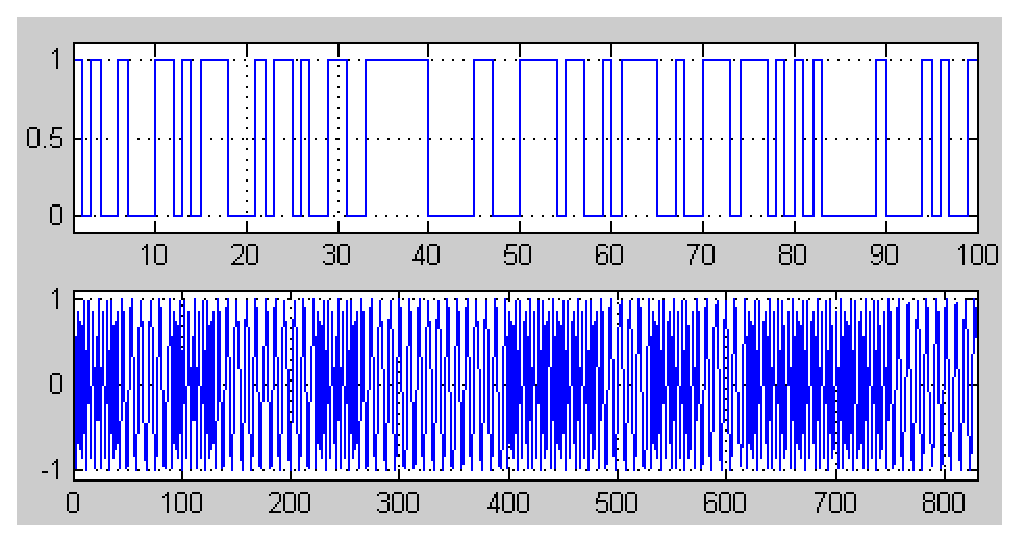
\includegraphics[width=8cm]{bilder/empfaenger/Sendesig}
	\caption{Bitstrom und Sendesignal}
	\label{fig:Sendesig}
\end{figure}

Jeder Bandpass hat die Aufgabe, eine der beiden Signalfrequenzen zu separieren, so dass pro Zweig nur noch eine einzige Frequenz detektiert werden kann. Somit liefert also in einem Zweig nur noch die der Null zugeordnete Frequenz einen Beitrag, im anderen Zweig die der Eins zugeordnete Frequenz. Dies ist in Abbildung \ref{fig:Bandpassig} dargestellt.

\begin{figure}[ht]
	\centering 
%	\psfrag{06}{$N$}
	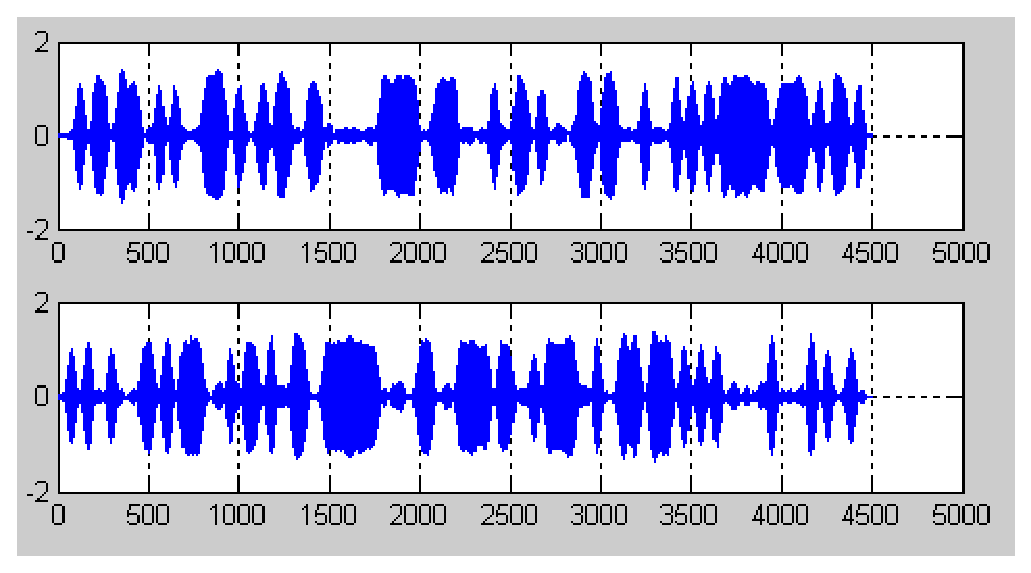
\includegraphics[width=8cm]{bilder/empfaenger/Bandpassgef}
	\caption{Bandpassgefilterte Signale}
	\label{fig:Bandpassig}
\end{figure}

Um nun wieder ein eindeutiges Signal zu erhalten, wird eine H�llkurven\-demodulation durchgef�hrt. Hier wird durch eine einfache Quadrierung des Signals die negative Halbwelle des Sinussignals nach oben ``geklappt'' (vgl. Abb. \ref{fig:Quadriertessig}) und danach mit einem Tiefpass gegl�ttet. Das Ergebnis ist in Abb. \ref{fig:quadutpgefsig} dargestellt.

\begin{figure}[ht]
	\centering 
%	\psfrag{06}{$N$}
	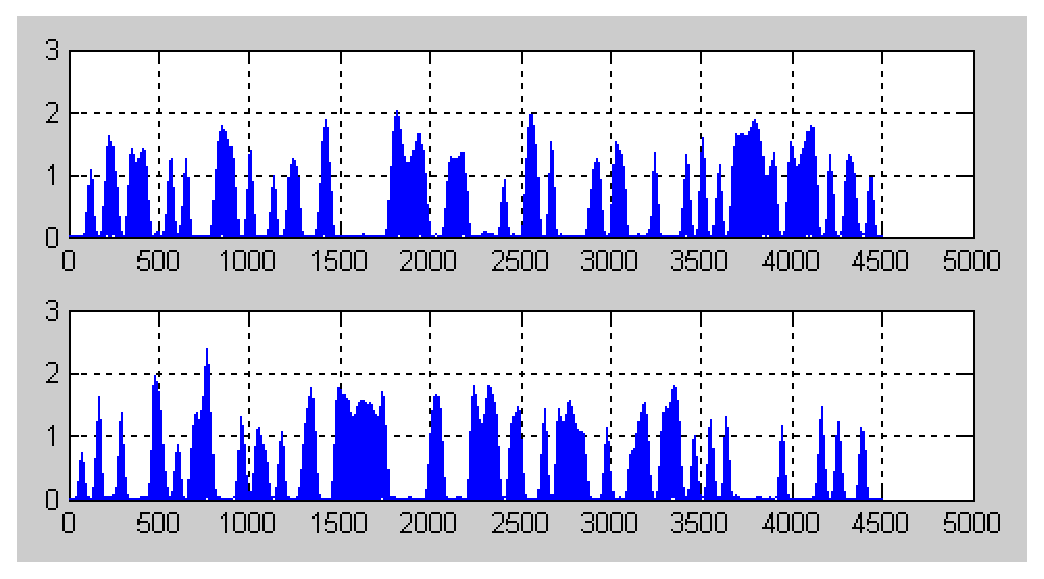
\includegraphics[width=8cm]{bilder/empfaenger/Quadriertessig}
	\caption{Bandpassgefiltertes und quadriertes Signal}
	\label{fig:Quadriertessig}
\end{figure}

\begin{figure}[ht]
	\centering 
%	\psfrag{06}{$N$}
	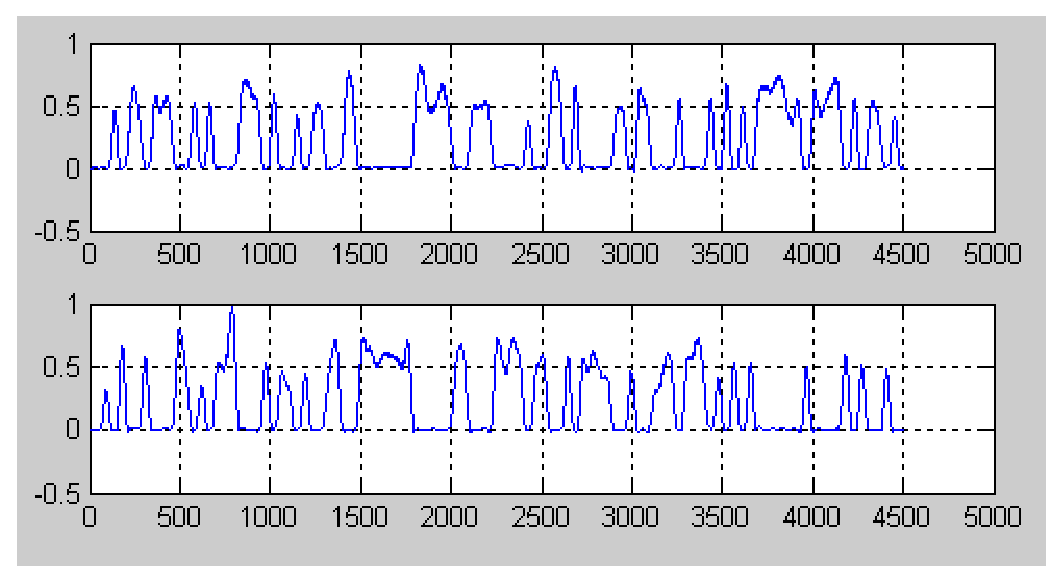
\includegraphics[width=8cm]{bilder/empfaenger/quadutpgefsig}
	\caption{Tiefpassgefiltertes Signal}
	\label{fig:quadutpgefsig}
\end{figure}

Zum Abschluss werden die beiden Signale noch von einander subtrahiert (vgl. Abb. \ref{fig:Empfangssignal}). Im Idealfall sollte das auf diese Weise rekonstruierte Signal dem zu Beginn erzeugten Bitstrom entsprechen.

\begin{figure}[ht]
	\centering 
%	\psfrag{06}{$N$}
	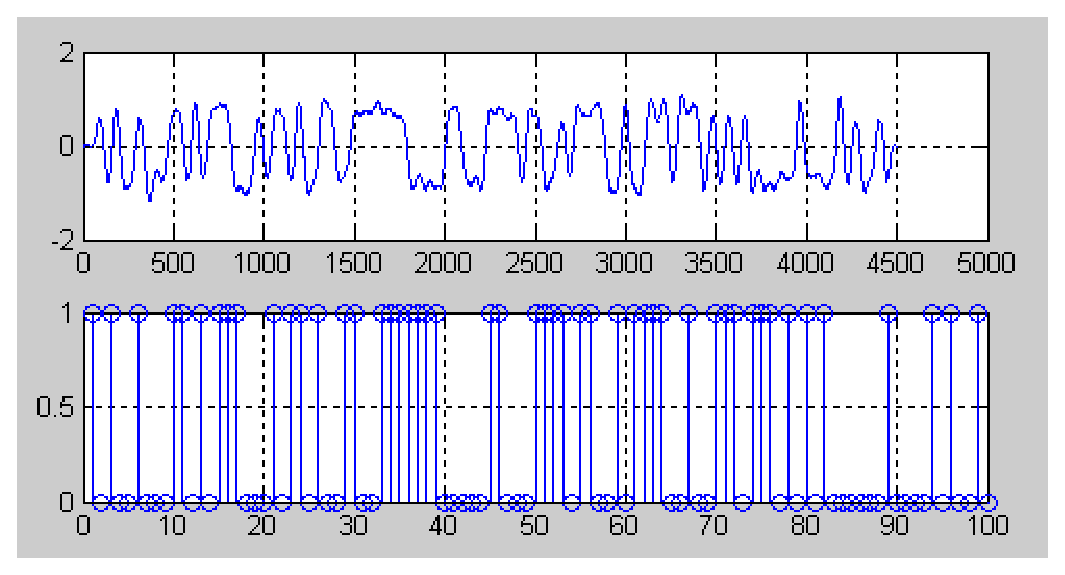
\includegraphics[width=8cm]{bilder/empfaenger/Empfangssig}
	\caption{Rekonstruiertes Empfangssignal}
	\label{fig:Empfangssignal}
\end{figure}

Sie werden nun in den folgenden Kapiteln nach und nach die einzelnen Bl�cke des Empf�ngers selbst entwerfen und die �bertragungsstrecke sowohl als Simulation als auch in Hardware aufbauen.
	\section{Grundlagen Digitaler Filter}\label{sec:digifilt}

%
%
%
%
\subsection{Einf�hrung}\label{subsec:digifilt:introduction}
%
%

Der Entwurf, die Realisierung und der Einsatz von digitalen Filtern ist das klassische Anwendungsgebiet der digitalen Signalverarbeitung. In der Theorie sind digitale Filter schon seit Beginn der 1970er Jahre bekannt. Allerdings konnten sie erst mit Aufkommen der DSPs in den 1980er Jahren an Popularit�t gewinnen.

\medskip Unter einem Filter versteht man ein System, das gewisse Frequenzkomponenten im Vergleich zu anderen ver�ndert, beispielsweise unterdr�ckt, verst�rkt oder in ihrer Phase verschiebt. Im Bereich der digitalen Filter spielen stabile und kausale LTI-Systeme\index{LTI-Systeme}, die durch rationale �bertragungsfunktionen mit reelen Koeffizienten beschrieben werden k�nnen, die wichtigste Rolle. Solche Filter werden meistens als \textit{lineare Digitalfilter}\index{lineare Digitalfilter} bezeichnet.

%
\subsubsection{Echtzeitsystem zur digitalen Filterung}
%

\begin{figure}[ht]
	\centering 
	\psfrag{01}{$x_{in}(t)$}
	\psfrag{04}{$x[n]$}
	\psfrag{06}{$y[n]$}
	\psfrag{09}{$y_{out}(t)$}
	\psfrag{10}{$f_s$}
	\includegraphics[width=13cm]{bilder/empfaenger/filter/DigiFilt}
	\caption{Echtzeitsystem zur digitalen Filterung}
	\label{fig:DigiFilt}
\end{figure}

Im Bild \ref{fig:DigiFilt} wird der grunds�tzliche Aufbau eines Echtzeitsystems zur digitalen Filterung dargestellt. Das zeitkontinuierliche Eingangssignal $x_{in}(t)$ wird zun�chst auf ein analoges Tiefpassfilter $TP_1$ gef�hrt, das der Bandbegrenzung dient (Antialiasing\index{Antialiasing}). Das bandbegrenzte Signal wird durch den folgenden AD-Wandler abgetastet und in die ``digitale Welt'' �bersetzt. Das Signal besteht nun aus einer Folge von Abtastwerten, die dem digitalen Filter zugef�hrt werden. Die Filterfunktion wird von einem Digitalrechner �bernommen, der aus den Eingangswerten $x[n]$ die Ausgangsfolgewerte $y[n]$ berechnet. Der DA-Wandler setzt das vom Filter ausgegebene Signal in eine zeitkontinuierliche, treppenf�rmige Spannung um. Anschlie�end wird es mit einem Tiefpassfilter $TP_2$ gegl�ttet und der wertekontinuierliche Verlauf zur�ckgegeben.

Die Tiefp�sse $TP_1$ und $TP_2$ sind Bandbegrenzungsfilter zur Unterdr�ckung hoher Frequenzen. W�nscht man zus�tzlich eine Unterdr�ckung der DC-Komponenten, wie zum Beispiel in der Audiosignalverarbeitung, dann werden sie durch Bandpassfilter ersetzt. 

%
\subsubsection{Grundlegende Filterfunktionen}\label{subsubsec:digifilt:filterfunctions}
%

F�r unsere Anwendung sind lediglich die klassischen Filter, wie Tiefpass-, Bandpass- und Hochpassfilter von Bedeutung. Die Funktion der Filter wird durch die schematische Darstellung der Amplituden-Frequenzg�nge in Abb. \ref{fig:amplitudenfreq} verdeutlicht.

\begin{figure}[ht]
	\centering 
	\psfrag{01}{$|H(f)|$}
	\psfrag{02}{Tiefpass}
	\psfrag{03}{$f$}
	\psfrag{04}{$f_{pass}$}
	\psfrag{05}{$f_{stop}$}
	\psfrag{06}{$0.5f_s$}
	\psfrag{07}{$|H(f)|$}
	\psfrag{08}{Bandpass}
	\psfrag{09}{$f_{stop1}$}
	\psfrag{10}{$f_{pass1}$}
	\psfrag{31}{$f_{pass2}$}
	\psfrag{12}{$f_{stop2}$}
	\psfrag{13}{$0.5f_s$}
	\psfrag{14}{$f$}
	\psfrag{15}{$|H(f)|$}
	\psfrag{16}{Hochpass}
	\psfrag{17}{$f_{stop}$}
	\psfrag{18}{$f_{pass}$}
	\psfrag{19}{$0.5f_s$}
	\psfrag{20}{$f$}
	\psfrag{21}{$|H(f)|$}
	\psfrag{22}{Bandsperre}
	\psfrag{23}{$f_{pass1}$}
	\psfrag{24}{$f_{stop1}$}
	\psfrag{25}{$f_{stop2}$}
	\psfrag{26}{$f_{pass2}$}
	\psfrag{27}{$0.5f_s$}
	\psfrag{28}{$f$}
	\includegraphics[width=13cm]{bilder/empfaenger/filter/filter}
	\caption{Filterfrequenzg�nge}
	\label{fig:amplitudenfreq}
\end{figure}

Die Parameter $f_{pass x}$ nennt man Durchlassfrequenzen\index{Durchlassfrequenzen}, die $f_{stop x}$ Sperrfrequenzen\index{Sperrfrequenzen}. Die drei Frequenzbereiche, die durch die Durchlass- und Sperrfrequenzen begrenzt werden heissen Durchlass-\index{Durchlassbereich}, �bergangs-\index{�bergangsbereich} und Sperrbereich\index{Sperrbereich}.

%
\subsubsection{Das Digitalfilter als LTI-System}\label{subsubsec:digifilt:lti}
%

Digitale Filter sind stabile, kausale LTI-Systeme, die sich mit einer rationalen �bertragungsfunktion beschreiben lassen: 
\begin{equation}
	H_z(z)=\cfrac{Y_z(z)}{X_z(z)}=\cfrac{b_0+b_1z^{-1}+...+b_Nz^{-N}}{1+a_1z^{-1}+...+a_Mz^{-M}}
	\label{math:�bertragungsfkt}
\end{equation}

Die \textit{�bertragungsfunktion}\index{�bertragungsfunktion} $H(z)$ definiert das �bertragungsverhalten des Systems und die gr��ere der beiden nat�rlichen Zahlen N und M legt ihre Ordnung fest. Sind alle rekursiven Koeffizienten $a_i$ gleich Null, so spricht man von einem \textit{nichtrekursiven LTI-System} oder einfach von einem \textit{FIR-Filter\index{FIR-Filter}}\footnote{Finite-Impulse-Response Filter}, andernfalls von einem \textit{rekursiven LTI-System} oder einem \textit{IIR-Filter}\index{IIR-Filter}\footnote{Infinite-Impulse-Response Filter}.

\medskip Unter dem \textit{Frequenzgang}\index{Frequenzgang} versteht man die �bertragungsfunktion, ausgewertet auf dem Einheitskreis der z-Ebene:
\begin{equation} 
	H(e^{j2\pi fT})=H(z)|_{e^{j2\pi fT}} 
\end{equation}
Den Betrag $|H(e^{j2\pi fT})|$ nennt man \textit{Amplitudengang}\index{Amplitudengang}, den Winkel $\angle H(e^{j2\pi fT})$ \textit{Phasengang}\index{Phasengang}. Die negative Ableitung des Phasengangs ist die \textit{Gruppenlaufzeit}\index{Gruppenlaufzeit}:
\begin{equation}
  \tau _g(e^{j2\pi fT})=-\cfrac{1}{2\pi}\cfrac{d\angle H(e^{j2\pi fT})}{df} 
\end{equation}
Die Gruppenlaufzeit charakterisiert die Verz�gerung eines LTI-Systems. Eine weitere, weniger gebr�uchliche, Gr��e ist die \textit{Phasenlaufzeit}\index{Phasenlaufzeit}:
\begin{equation}
	\tau_p(e^{j\Omega}=-\cfrac{arg(H(\Omega))}{\Omega}=-\cfrac{\angle H(e^{j\Omega})}{\Omega}\textnormal{ mit }\Omega=2\pi fT
\end{equation}

Mit diesem Parameter kann die Reaktion eines LTI-Systems auf eine sinusf�rmige Eingangsgr��e der Frequenz $\Omega$ im eingeschwungenen Zustand in der Form
\begin{equation}
	y[n]=\lvert H(\Omega)\rvert cos(\Omega(n-\tau_p))
\end{equation}
geschrieben werden. \\Die Phasenlaufzeit ist somit gleich der Anzahl der Abtastintervalle, mit der eine Sinusschwingung beim Durchlaufen eines zeitdiskreten LTI-Systems verz�gert wird. \\Die Gruppenlaufzeit dagegen ist gleich der Anzahl der Abtastintervalle, um die die H�llkurve eines modulierten Systems verz�gert wird.

\medskip Transformieren wir die �bertragungsfunktion in den Zeitbereich, so erh�lt man die Impulsantwort $h[n]$:
\begin{equation} 
	H(z) \ifouriersymb h[n]
\end{equation}
Im Frequenzbereich ist das Ausgangssignal gleich dem Eigangssignal multipliziert mit der �bertragungsfunktion,
\begin{equation}
	Y(z)=H(z)X(z)
	\label{math:EmultH}
\end{equation}
im Zeitbereich gleich dem Eingangssignal gefaltet mit der Impulsantwort.
\begin{equation} 
	y[n]=h[n]\ast x[n]
\end{equation}
Setzen wir f�r $H(z)$ in Gl. (\ref{math:EmultH}) die rationale Funktion (\ref{math:�bertragungsfkt}) ein, f�hrt die R�cktransformation auf die \textit{Differenzengleichung}\index{Differenzengleichung}:
\begin{equation}
	y[n]=-\sum_{i=0}^M a_iy[n-i]+\sum_{i=0}^N b_ix[n-i]
	\label{math:Differenzengleichung}
\end{equation}
Betrachtet man die Differenzengleichung genauer, so kann man leicht erkennen, dass diese mit Hilfe  einfacher Addierer, Multiplizierer und Verz�gerungsglieder in Hardware realisierbar ist.


Letztendlich kann man die �bertragungsfunktion noch in einer \textit{Pol-Null\-stel\-len-Dar\-stel\-lung}\index{Pol-Nullstellen-Darstellung} angeben: 
\begin{equation}
	H_z(z)=b_0z^{M-N}\cfrac{(z-z_1)(z-z_2)...(z-z_N)}{(z-p_1)(z-p_2)...(z-p_M)}
  \label{math:PolNullstellen}
\end{equation}
Die Parameter $p_i$ werden als \textit{Pole}\index{Pole} bezeichnet, die $z_i$ als \textit{Nullstellen}\index{Nullstellen}.

\paragraph*{Zusammenfassung:} Ein lineares Digitalfilter beschreibt man gew�hnlich mit Hilfe seiner �bertragungsfunktion. Aus ihr lassen sich die wichtigsten Funktionen und Gesetzm�ssigkeiten einfach ableiten.

Aufgabe des Filterentwurfs ist es, die Ordnung und die Koeffizienten der Filter�bertragungsfunktion zu einem vorgegebenen Zielfrequenzgang zu bestimmen. Wir werden in der Folge geeignete Methoden dazu diskutieren.

%
%
\subsection{Eigenschaften und Strukturen von FIR-Filtern}\label{subsec:digifilt:fir}\index{FIR-Filter}
%
%

Wie oben schon angesprochen teilt man die digitalen Filter in FIR- und IIR-Filter ein. Beide Klassen haben interessante Eigenschaften, wobei wir uns in diesem Praktikum auf die Verwendung von FIR-Filtern beschr�nken werden. 

Die Struktur der Filter beschreibt man h�ufig in Form eines Signalflussdiagramms\index{Signalflussdiagramm} oder auch eines Blockdiagramms\index{Blockdiagramm}. Kennen wir diese, so sind wir in der Lage ein Programm zu schreiben und digitale Filter auf einem Rechner zu implementieren. 

%
\subsubsection{Grundlagen}\label{subsubsec:digifilt:fir:basics}
%

Die Differenzengleichung eines FIR-Filters lautet:
\begin{equation}
	y[n]=\sum_{i=0}^Nb_ix[n-i]
\end{equation}
Damit k�nnte ein nichtrekursives FIR-System 3. Ordnung folgenderma�en aussehen:
\begin{equation}
y[n]=b_0x[n]+b_1x[n-1]+b_2x[n-2]+b_3x[n-3]
\end{equation}


\begin{figure}[ht]
	\centering 
	\psfrag{01}{$x[n]$}
	\psfrag{02}{$y[n]$}
	\psfrag{03}{$b_0$}
	\psfrag{04}{$b_1$}
	\psfrag{05}{$b_2$}
	\psfrag{06}{$b_3$}
	\includegraphics[width=13cm]{bilder/empfaenger/filter/FIR3}
	\caption{FIR-Filter 3. Ordnung}
	\label{fig:FIR3}
\end{figure}

Anhand dieses einfachen Beispiels kann man erkennen, dass die Impulsantwort eines nichtrekursiven LTI-Systems N-ter Ordnung gleich den Koeffizienten der Differentialgleichung ist. Die L�nge der Impulsantwort ist dann $N+1$:
\begin{equation}
	h[n]={h_0,h_1,...,h_N}={b_0,b_1,...,b_N}
\end{equation}
Diese endliche L�nge f�hrte zur Bezeichnung FIR-Filter (Finite-Impulse-Response-Filter).

Die �bertragungsfunktion lautet allgemein:
\begin{equation}
	H(z)=b_0+b_1z^{-1}+...+b_Nz^{-N}
	\label{math:FIR�bertragungsfkt}
\end{equation}

Durch Erweiterung mit $z^N$ kann die �bertragungsfunktion auch in der Form
\begin{equation}
	H(z)=\cfrac{b_0z^N+b_1z^{N-1}+...+b_N}{z^N}
\end{equation}
geschrieben werden. Daraus geht hervor, dass alle Pole im Ursprung liegen und dass das FIR-Filter somit immer stabil ist.

%
\subsubsection{Eigenschaften von FIR-Filtern}\label{subsubsec:digifilt:fir:characteristics}
%

Alle Entwurfsverfahren liefern symmetrische FIR-Filter, deren Impulsantwort immer spie\-gel- oder punktsymmetrisch ist (vgl. Abb. \ref{fig:FIRSymm}).

\begin{figure}[ht]
	\centering 
	\psfrag{01}{$h[n]$}
	\psfrag{02}{$n$}
	\psfrag{03}{$\cfrac{N}{2}$}
	\psfrag{04}{$1$}
	\psfrag{05}{$0$}
	\psfrag{06}{$N$}
	\includegraphics[width=9cm]{bilder/empfaenger/filter/FIRImpulsantw}
	\caption{Symmetrieeigenschaften von FIR Filter}
	\label{fig:FIRSymm}
\end{figure}

Symmetrische FIR-Filter haben, abgesehen von 180\textdegree-Phasenspr�ngen, einen linearen Phasengang. Daher werden sie auch als linearphasige Filter bezeichnet. Die Gruppenlaufzeit $\tau_g(f)$ symmetrischer Filter ist konstant und ihr Wert gleich NT/2. Es kommt also zu keinen Gruppenlaufzeitverzerrungen! 

Filter mit konstanter Gruppenlaufzeit haben die angenehme Eigenschaft, dass sie Signale im Durchlassbereich nur verz�gern, aber nicht verzerren. Zudem bleibt die Symmetrie symmetrischer Pulse erhalten, was f�r viele Anwendungen vorteilhaft ist.

\paragraph{Beispiel:} Hier als Beispiel ein linearphasiger FIR-Tiefpass (vgl. Abbildungen \ref{fig:FIRTP} bis \ref{fig:FIRTPFrequber}):

\begin{figure}[ht]
	\centering 
	\includegraphics[width=8cm]{bilder/empfaenger/filter/LinTPFilter}
	\caption{Frequenzgang eines linearphasigen TP-Filters}
	\label{fig:FIRTP}
\end{figure}

\begin{figure}[ht]
	\centering
		\includegraphics[width=7cm]{bilder/empfaenger/filter/LinTPImpulsantw}
	\caption{Im\-puls\-ant\-wort eines linearphasigen TP-Fil\-ters}
	\label{fig:FIRTPImpulsantw}
\end{figure}

\begin{figure}[ht]
	\centering
		\includegraphics[width=7cm]{bilder/empfaenger/filter/LinTPPolNst}
	\caption{Pol-Null\-stel\-len\-dia\-gramm eines linearphasigen TP-Fil\-ters}
	\label{fig:FIRTPPolNst}
\end{figure}

Es handelt sich um ein linearphasiges Tiefpassfilter. Abgesehen von 180\textdegree-Pha\-sen\-spr�n\-gen (die an den Nullstellen des Amplitudengangs auftreten und daher keinen Einfluss auf das �bertragungsverhalten haben) ist der Phasengang linear. Die L�nge des Filters ist 22, demnach muss die �bertragungsfunktion 21 Nullstellen und 21 im Ursprung liegende Pole haben.

\begin{figure}[ht]
	\centering 
%	\psfrag{06}{$N$}
	\includegraphics[width=9cm]{bilder/empfaenger/filter/LinTPZeitber}
	\caption{Ein- und Ausgangsverhalten bei Anregung mit einem punktsymmetrischen Doppelrechteckpuls: Zeitbereich}
	\label{fig:FIRTPZeitber}
\end{figure}

Der tiefpassgefilterte Rechteckimpuls ist erwartungsgem�� an seinen Ecken abgerundet, aber immer noch punktsymmetrisch (vgl. Abb. \ref{fig:FIRTPZeitber}). Der Schwerpunkt des Ausgangs-Pulses ist gegen�ber dem Schwerpunkt des Eingangs-Pulses um die Gruppenlaufzeit \\$\tau_g$ = 1.05 ms verz�gert.

\begin{figure}[ht]
	\centering 
%	\psfrag{06}{$N$}
	\includegraphics[width=7cm]{bilder/empfaenger/filter/LinTPFrequber}
	\caption{Ein- und Ausgangsverhalten im Frequenzbereich}
	\label{fig:FIRTPFrequber}
\end{figure}

\develnote{Wenn noch Zeit ist sollten die Graphiken noch ein bisschen aufgem�belt werden!}

%
\subsubsection{Strukturen von FIR-Filtern}\label{subsubsec:FIRStrukturen}
%
Am einfachsten l�sst sich das Filter in einer Straight-Forward-Implementierung realisieren, indem man die Differenzengleichung 1:1 umsetzt. Diese Form nennt sich Direktform- \index{Direktformstruktur}oder Transversalfilterstruktur\index{Transversalfilterstruktur} (vgl. Abb. \ref{fig:FIRDirektform}).

\begin{figure}[ht]
	\centering 
%	\psfrag{06}{$N$}
	\includegraphics[width=13cm]{bilder/empfaenger/filter/FIRDirektform}
	\caption{Direktform- oder Transversalfilterstruktur bei FIR-Filtern}
	\label{fig:FIRDirektform}
\end{figure}
\medskip Durch Ausnutzung der Symmetrie kann man etwa die H�lfte der Multiplikationen einsparen (vgl. Abb. \ref{fig:FIRLinearphasenstruktur}).

\begin{figure}[ht]
	\centering  
%	\psfrag{06}{$N$}
	\includegraphics[width=13cm]{bilder/empfaenger/filter/FIRLinearphasenstruktur}
	\caption{Linearphasenstruktur eines FIR-Filters}
	\label{fig:FIRLinearphasenstruktur}
\end{figure}
Die Differenzengleichung lautet dann: 
\begin{equation}
	y[n]=b_0(x[n]+x[n-N])+b_1(x[n-1]+x[n-N+1])+...+b_{N/2}x[n-N/2]
\end{equation}

%
\subsection{Entwurf von FIR-Filtern}\label{subsec:digifilt:fir:design}
%
Man beginnt das Filterdesign mit der Spezifikation der einzelnen Filtergrenzfrequenzen. Da Filter mit rechteckf�rmigen Amplitudeng�ngen eine unendlich hohe Ordnung besitzen w�rden, sind sie in der Praxis nicht realisierbar. Man legt daher, wie beim Bandpass in Abb. \ref{fig:FIREntwurf} dargestellt, einen Toleranzbereich\index{Toleranzbereich} fest, in dem sich der Amplitudengang des Filters befinden darf.

\begin{figure}[ht]
	\centering 
	\psfrag{01}{$|H(f)|$}
	\psfrag{02}{$f$}
	\psfrag{03}{$1+\delta_1$}
	\psfrag{04}{$1-\delta_1$}
	\psfrag{05}{$f_{stop1}$}
	\psfrag{06}{$f_{pass1}$}
	\psfrag{07}{$f_{pass2}$}
	\psfrag{08}{$f_{stop2}$}
	\psfrag{09}{$0.5f_s$}
	\psfrag{10}{$\delta_2$}
	\includegraphics[width=13cm]{bilder/empfaenger/filter/FIREntwurf}
	\caption{Toleranzschema des Amplitudengangs}
	\label{fig:FIREntwurf}
\end{figure}

Die maximal zul�ssigen Abweichungen $\delta_1$ und $\delta_2$ vom idealen Amplitudengang hei�en \textit{Rippel}\index{Rippel} im Durchlass- bzw. Sperrbereich. Die Bereiche, die durch das Festlegen der Grenzfrequenzen entstehen, nennt man Durchlass-\index{Durchlassbereich}, �bergangs-\index{�bergangsbereich} und Sperrbereich\index{Sperrbereich}. Die zugeh�rigen Grenzfrequenzen\index{Grenzfrequenzen} hei�en Durchlass-\index{Durchlassfrequenzen} und Sperrfrequenzen\index{Sperrfrequenzen}. 

�blicherweise wird nur der Frequenzbereich von 0 bis $f_s/2$ bzw. von 0 bis $\pi$ dargestellt, da sich danach der Frequenzgang wiederholt. 

Die Wahl eines geeigneten Toleranzschemas\index{Toleranzschema} ist eine typische Ingenieursaufgabe und h�ngt von der Anwendung des Filters ab. 

Allgemein gilt, dass die Ordnung, und damit die Komplexit�t des Filters, steigt, je enger das Toleranzschema gew�hlt wird. F�r eine gegebene Anwendung wird der Toleranzbereich daher so gro� wie m�glich gew�hlt, um die Filterordnung und somit auch die Zahl der n�tigen Multiplikationen klein zu halten. 

Die beiden wichtigsten Entwurfsmethoden f�r FIR-Filter sind die
\begin{itemize}
	\item Fenstermethode\index{Fenstermethode} und die
	\item Optimalmethode\index{Optimalmethode}\index{Equirippleverfahren} (auch Equi\-ripple-Ver\-fah\-ren, Re\-mez-Ent\-wurf oder Che\-by\-chev-Ap\-proxi\-mation genannt).
\end{itemize}

%
\subsubsection{Filterentwurf mit der Fenstermethode}\label{subsubsec:digifilt:fir:design:window}\index{Fenstermethode}
%
\paragraph*{Entwurfsschritte der Fenstermethode}
\begin{enumerate}
\item Festlegen der Eck\-fre\-quenz(en)\index{Eckfrequenzen} des idealen recht\-eck\-f�rmigen Filter\-frequenzgangs \\ $H_{ideal}(\Omega)$.
\item Berechnen (oder nachlesen in Tabellen) der entsprechenden Filter\-impuls\-antwort $h_{ideal}(n)$ (diese ist unendlich lang und nicht kausal und daher nicht realisierbar)
\item Multiplizieren der idealen Impulsantwort $h_{ideal}(n)$ mit einer geeigneten Fenster\-funktion\index{Fensterfunktion} $w[n]$
\begin{equation}
h[n]=h_{ideal}[n]\cdot w[n]
\end{equation}
\item Verz�gern der resultierenden Impulsantwort $h[n]$, so dass ein kausales (realisierbares) System entsteht.
\end{enumerate}

\clearpage
\paragraph*{Ideale Impulsantworten der grundlegenden Filterfunktionen}
\begin{itemize}
	\item Idealer Tiefpass mit der Eckfrequenz $\Omega_c$
	\begin{equation}
		h_{ideal}[n]=\cfrac{\Omega_c}{\pi}sinc(n\Omega_c)
	\end{equation}
	\item Idealer Bandpass mit den Eckfrequenzen $\Omega_1$ und $\Omega_2$
	\begin{equation}
		h_{ideal}[n]=\cfrac{\Omega_2}{\pi}sinc(n\Omega_2)-\cfrac{\Omega_1}{\pi}sinc(n\Omega_1)
	\end{equation}
\end{itemize}

In den Abb. (\ref{fig:FensterZeitber}) und (\ref{fig:FensterFrequber}) ist der Entwurfsablauf mit der Fenstermethode im Zeit- und Frequenzbereich dargestellt.

\begin{figure}[ht]
	\centering 
	\psfrag{A}{Ideale Impulsantwort}
	\psfrag{B}{Fenster}
	\psfrag{C}{Gefensterte Impulsantwort}
	\psfrag{D}{Verz�gerte Impulsantwort}
	\includegraphics[width=8cm]{bilder/empfaenger/filter/FenstermethodeZeitber}
	\caption{Fenstermethode im Zeitbereich}
	\label{fig:FensterZeitber}
\end{figure}

\begin{figure}[ht]
	\centering 
	\psfrag{A}{Ideale Impulsantwort}
	\psfrag{B}{Impulsantwort des Fensters}
	\psfrag{C}{Gefensterte Impulsantwort}
	\psfrag{D}{Verz�gerte Impulsantwort}
	\includegraphics[width=8cm]{bilder/empfaenger/filter/FenstermethodeFrequber}
	\caption{Fenstermethode im Frequenzbereich}
	\label{fig:FensterFrequber}
\end{figure}



\paragraph*{Zur Wahl des Fensters:}

F�r die Fenstermethode stehen unterschiedliche Fenstertypen zur Verf�gung. Hier sind drei der Gebr�uchlichsten aufgef�hrt. Informationen zu weiteren Fenstertypen finden sie unter anderem in der Online-Hilfe von MATLAB.

\begin{itemize}
	\item Rechteckfenster:\index{Rechteckfenster}
	\begin {itemize}
		\item hat gro�e Rippel im Amplitudengang zur Folge
		\item Das Toleranzschema resultiert nicht aus dem Input des Entwurfs, sondern ist das mehr oder weniger zuf�llige Resultat des Entwurfs
	\end{itemize}
	\item Hanningfenster:\index{Hanningfenster}
	\begin {itemize}
		\item Die Rippel im Durchlassbereich sind deutlich kleiner als beim Entwurf mit einem Rechteckfenster
		\item Wie schon beim Entwurf mit dem Rechteckfenster ist das Toleranzschema nicht der Input des Entwurfs, sondern ein mehr oder weniger zuf�lliges Resultat
	\end{itemize}
	\item Kaiserfenster:\index{Kaiserfenster}
	\begin {itemize}
		\item Zus�tzlich zur Fensterl�nge kann ein zus�tzlicher Parameter ($\beta$) frei gew�hlt werden
		\item Dies erm�glicht, dass mit dem Kaiserfenster tats�chlich das Toleranzschema vorgegeben werden kann. Die beiden Parameter $N+1$ (Fensterl�nge) und $\beta$ k�nnen in der Folge bestimmt werden, das Endresultat des Entwurfs sind wiederum die Ordnung\index{Ordnung} N des Filters sowie die Filterkoeffizienten\index{Filterkoeffizienten} $b_0,...,b_n$
		\item Die Filterordnung ist �blicherweise relativ hoch, da das Toleranzschema nicht optimal ausgenutzt wird
	\end{itemize}
\end{itemize}

Eine graphische Darstellung hierzu finden sie in Abb. \ref{fig:Fenstertypen}.

\begin{figure}[ht]
	\centering 
	\psfrag{A}{Rechteckfenster}
	\psfrag{B}{Kaiserfenster}
	\psfrag{C}{Hanningfenster}
	\includegraphics[width=7cm]{bilder/empfaenger/filter/Fenstertypen}
	\caption{Fenstertypen}
	\label{fig:Fenstertypen}
\end{figure}

%
\subsubsection{Filterentwurf mit der Optimalmethode}\label{subsubsec:digifilt:fir:design:optimal}\index{Optimalmethode}
%

Mit dieser Methode lassen sich Filter entwerfen, die eine gleichm��ige Welligkeit\index{Welligkeit} im Durchlass- und Sperr\-bereich aufweisen. Dabei nutzen sie den gesamten Toleranzbereich aus. Die daraus resultierende Filterordnung N ist im Allgemeinen wesentlich kleiner, als diejenige des Fensterentwurfs. Die Theorie hinter der Optimalmethode ist sehr umfangreich und w�rde den Rahmen des Praktikums sprengen. Allerdings wird die Optimalmethode als Standardverfahren von vielen Programmpaketen zur Signalverarbeitung unterst�tzt. 

Die Optimalmethode erm�glicht nicht nur den Entwurf der vier Filtergrundarten, sondern auch den Entwurf von Multibandfiltern, Differentiatoren u.a.

%
%
\subsection{Nichtideale Effekte bei digitalen Filtern}\label{subsec:digifilt:nonideal}
%
%

%
\subsubsection{Quantisierungsrauschen durch AD-Wandlung}\label{subsubsec:digifilt:nonideal:quantnoise}
%
Bei der AD-Wandlung wird das analoge Signal zun�chst abgetastet und in ein zeitdiskretes Signal �berf�hrt. Dieses wird in einem zweiten Schritt mit Hilfe einer Quantisierungs\-kennlinie bewertet. Das resultierende digitale Signal ist jetzt zeit- und wertediskret.

Da digitale Signale, je nach Wortl�nge, nur bestimmte Werte annehmen k�nnen, muss das Analogsignal entsprechend abgeschnitten oder gerundet werden. In jedem Fall geht bei diesem Schritt ein geringer Teil der Information verloren, weshalb das urspr�ngliche Signal nicht mehr fehlerfrei rekonstruiert werden kann. Man spricht von einem \textbf{Quantisierungsfehler}\index{Quantisierungsfehler}. Je gr��er die Wortl�nge des AD-Wandlers ist, desto geringer f�llt der resultierende Fehler aus. 

\paragraph{Quantisierungsrauschen:}
Man kann den Quantisierungsfehler als ein Zufallssignal $e[n]$ modellieren, das durch die Quantisierung entsteht und deshalb als Quantisierungsrauschen bezeichnet wird:
\begin{equation}
	x_Q[n]=x[n]+e[n]
\end{equation}
Das quantisierte Signal $x_Q[n]$ kann als �berlagerung des amplitudenkontinuierlichen Signals $x[n]$ und des Fehlersignals $e[n]$ aufgefasst werden. 

\medskip Ein Qualit�tsma� in der Signalverarbeitung ist der sogenannte Signal-Rauschabstand SNR (Signal to Noise Ration):
\begin{equation}
	SNR_{dB} = 10\cdot log\left(\cfrac{P_S}{P_N}\right)
\end{equation}
mit: $P_S$ $\rightarrow$ Mittlere Leistung des Nutzsignals $x[n]$\\
\textcolor{white}{mit:} $P_N$ $\rightarrow$ Mittlere Leistung des Fehlersignals $e[n]$

\medskip F�r den Sonderfall, dass das Eingangssignal symmetrisch gleichf�rmig mit der Aufl�sung B (Anzahl und Bits) quantisiert wird und im gesamten Aussteuerbereich gleichverteilt ist, gilt:
\begin{equation}
	SNR_{dB} \approx B\cdot 6dB
\end{equation}
$\rightarrow$ Jede Erh�hung der Aufl�sung um 1 Bit verbessert also den Abstand zwischen Nutzanteil und Quantisierungs\-rauschen um 6dB!
%


\subsubsection{Quantisierung der Filterkoeffizienten}\label{subsubsec:digifilt:nonideal:koeffquant}\index{Filterkoeffizienten}\index{Quantisierung}
%

Die Entwurfsverfahren f�r digitale Filter liefern die $b$- und $a$-Koeffizienten der �bertragungsfunktion
\begin{equation}
	H_z(z)=\cfrac{b_0+b_1z^{-1}+...+b_Nz^{-N}}{1+a_1z^{-1}+...+a_Mz^{-M}}
	\label{math:�bertragungsfkt2}
\end{equation}
mit gro�er Genauigkeit (meist in Double-Precision-Floating-Point). Bei der Implementierung in Hard- oder Software k�nnen die Koeffizienten aber nur mit einer begrenzten Anzahl von Bits dargestellt werden, und aufgrund der g�nstigeren Komponenten meist auch nur in Fixed-Point-Darstellung. Die Folgen dieser reduzierten Genauigkeit k�nnen zum Beispiel
\begin{itemize}
	\item eine Verletzung der Entwurfsspezifikation nach der Quantisierung oder
	\item Instabilit�ten ehemals stabiler Filter bei IIR-Systemen 
\end{itemize}
sein.

\paragraph{FIR-Filter:}\index{FIR-Filter}

Bei FIR-Filtern der L�nge N entsprechen die Filterkoeffizienten der Impuls\-antwort\index{Impulsantwort}:
\begin{equation}
	h[n]=
	\begin{cases}
		b_n	&
		\textnormal{f�r } n=0,1,...,N\\
		0	&
		\textnormal{sonst}
	\end{cases}
\end{equation}
Die Quantisierung der Filterkoeffizienten wirkt sich also direkt auf die Impulsantwort des Systems aus und damit auf die �bertragungsfunktion und den Frequenzgang.

\medskip Fasst man die Koeffi\-zienten-Quanti\-sierungs\-fehler\index{Quantisierungsfehler} als additive St�rgr��e\index{St�rgr��e} $\Delta h[n]$ auf, so resultiert das Modell einer Parallelschaltung aus dem unquantisierten, also dem idealen System, und der St�rung durch die Koeffizientenquantisierung (vgl. Abb. \ref{fig:FIRquantkoeff})
\begin{equation}
	h_Q[n]=h[n]+\Delta h[n]
\end{equation}

\begin{figure}[ht]
	\centering 
	\psfrag{01}{$h[n]$}
	\psfrag{02}{$\Delta h[n]$}
	\psfrag{03}{$x[n]$}
	\psfrag{04}{$y[n]$}
	\includegraphics[width=7cm]{bilder/empfaenger/filter/quantkoeff}
	\caption{Fehlermodell f�r quantisierte Koeffizienten}
	\label{fig:FIRquantkoeff}
\end{figure}

\develnote{Absch�tzungsrechnung auf S. 110???}

Damit gilt f�r die obere Schranke des Fehlers im Frequenzgang:
\begin{equation}
	\underset{\Omega}{max}\lvert \Delta H(\Omega)\rvert \le (N+1)\cfrac{LSB}{2}
\end{equation}
F�r diese Absch�tzung wurde die sehr pessimistische Annahme unterstellt, dass sich alle Quantisierungsfehler der einzelnen Koeffizienten ung�nstig �berlagern. Insbesondere bei langen Impulsantworten kompensieren sich die Fehler zum Teil. Daher arbeiten realistische Absch�tzungen meist mit stochastischen Modellen. In der Praxis sollte man in JEDEM Fall vor der Implementierung das Filter simulieren!

\paragraph{IIR-Filter:}\index{IIR-Filter}

Auf IIR-Filter und die bei der Koeffizientenquantisierung entstehenden Probleme soll hier nicht weiter eingegangen werden, da wir aufgrund der deutlich besseren Stabilit�t ausschlie�lich mit FIR-Strukturen arbeiten werden. N�heres hierzu kann man allerdings in \cite{DigiSig} oder in \cite{ADS} nachlesen.

%
\subsubsection{Quantisierte Arithmetik}\label{subsubsec:digifilt:nonideal:arithquant}\index{Quantisierte Arithmetik}
%

Die Quantisierung der Filterkoeffizienten �ndert ``nur'' die �bertragungsfunktion und kann prinzipiell schon im Filterentwurf ber�cksichtigt werden. Wortl�ngeneffekte bei den arithmetischen Operationen treten dagegen w�hrend des Betriebs auf und k�nnen sehr unsch�ne Effekte verursachen. 

\medskip Lineare Digitalfilter bestehen aus Addierern, Verz�gerungsgliedern und Multiplizierern. Sowohl die Additionen als auch die Multiplikationen sind von der Quantisierung direkt betroffen.

\medskip Realisiert man ein Digitalfilter in Gleitkommadarstellung\index{Gleitkommadarstellung}, so k�nnen Quantisierungsfehler in der Regel ausgeschlossen werden und auch �berl�ufe brauchen nicht ber�cksichtigt zu werden, da sie vernachl�ssigbar klein sind. 

\medskip Bei der Realisierung in Festkommadarstellung\index{Festkommadarstellung} dagegen k�nnen bei der Addition \textit{�berl�ufe}\index{�berl�ufe} und in der Folge \textit{gro�e Grenzzyklen}\index{gro�e Grenzzyklen} entstehen. 

Bei der Multiplikation kann es zu \textit{Rundungsfehlern}\index{Rundungsfehler} kommen, die \textit{kleine Grenzzyklen}\index{kleine Grenzzyklen} nach sich ziehen. Da man bei Fest\-komma\-im\-ple\-men\-tie\-rung\-en allerdings in der Regel Abtastwerte und Koeffizienten als Fractional-Zahlen darstellt liegen die Ergebnisse von Multiplikationen im Bereich von [-1,1[, wodurch �berl�ufe vermieden werden (Ausnahme: $(-1)\cdot(-1)=1$).

\paragraph{Grenzzyklen:}\index{Grenzzyklen}

Bei der Implementierung digitaler Systeme mit endlicher Wortl�nge k�nnen parasit�re Schwingungen beobachtet werden, die trotz Stabilit�t der Filter auftreten. Diese Oszillationen werden Grenzzyklen oder Limit-Cycles genannt und entstehen durch Nicht\-linearit�ten in den R�ckkoppelschleifen der Filter. Man unterscheidet
\begin{description}
	\item[Kleine Grenzzyklen] (auch Granulargrenzzyklen) mit kleinen Amplituden, deren Ursache die Quantisierung bei Multiplikationen im R�ckkoppelzweig ist und
	\item [Gro�e Grenz\-zyklen] (auch �ber\-lauf\-grenz\-zyklen) mit gro�en Ampli\-tuden, die durch eine �berlauf\-behandlung bei Additionen in den R�ck\-kopplungen hervorgerufen werden. 
\end{description}

Da Grenzzyklen nur bei Filterstrukturen mit R�ckkopplung entstehen k�nnen sollen sie hier nur kurz angerissen werden. F�r eine genauere Betrachtung sei auf die einschl�gige Literatur verwiesen.

Das Auftreten dieser Effekte h�ngt von verschiedenen Parametern ab:
\begin{itemize}
	\item Filterkoeffizienten (steile und schmalbandige Filter neigen mehr dazu)
	\item Inhalt der Verz�gerungselemente vor dem Einschalten
	\item Eingangssignal (z.B. Zero-Input-Limit-Cycles)
	\item Filterstruktur
	\item Skalierung
	\item Wortl�nge
	\item Quantisierungsart bzw. �berlaufkennlinie
\end{itemize}	

\paragraph{Kleine Grenzzyklen:}

Sowohl beim Runden, als auch beim Abschneiden entstehen Fehler (Rundungsfehler oder Quantisierungsfehler). W�hrend beim Betragsabschneiden die Wortl�ngenverk�rzung stets zur Null hin vorgenommen wird, der Betrag der Zahl durch die Quantisierung also nicht zunehmen kann, wirkt eine Quantisierung mit Runden beim Aufrunden wie eine zus�tzliche Signalquelle, die dem System zus�tzliche Energie zuf�hrt und zu kleinen Grenzzyklen f�hren kann. Bei Quantisierung mit Betragsabschneiden wird dem System keine zus�tzliche Energie zugef�hrt, kleine Grenzzyklen werden auf Kosten einer gr��eren Ungenauigkeit vermieden.

\medskip Da kleine Grenzzyklen nur im Zusammenhang mit einer R�ckkopplung auftreten k�nnen sind sie f�r uns uninteressant. Lediglich bei Verwendung von IIR-Filtern sollte man diesen Effekt im Hinterkopf behalten.

\paragraph{Gro�e Grenzzyklen:}
Gro�e Grenzzyklen sind weitaus unangenehmer, da ihre Amplitude den gesamten Aussteuerbereich umfassen kann. Das Auftreten gro�er Grenzzyklen macht daher die Ergebnisse der Filterung komplett unbrauchbar. M�gliche Gegenma�nahmen sind:
\begin{itemize}
	\item \textbf{S�ttigungskennlinien:} In diesem Fall wird bei einem positiven oder negativen �berlauf die gr��te bzw. die kleinste darstellbare Maschinenzahl gesetzt. 
	\item Geeignete \textbf{Skalierung der Filterkoeffizienten}.
\end{itemize}

\paragraph{Skalierung von FIR-Filtern (zur Vermeidung von �berl�ufen):}
Da eine Skalierung der Filterkoeffizienten nur bei Filtern in Direktform-Struktur einen Effekt erzielen w�rde soll hier nur kurz auf diese M�glichkeit eingegangen werden. In den sp�teren Versuchen wird das Filter in einer Linearphasenstruktur implementiert, die durch diese Entwurfsmodifikation nicht zu beeinflussen ist.

\medskip Betrachtet man ein FIR-Filter in Direktform-\index{Direktform-Struktur} oder Trans\-versal\-struktur \index{Transversal-Struktur}(vgl. Abb. \ref{fig:FIRDirektform}), so sieht es auf den ersten Blick so aus, als m�sste f�r jeden einzelnen Summen\-knoten daf�r gesorgt werden, dass an dessen Ausgang kein �berlauf auftreten kann. Da Teil�berl�ufe bei der Summenbildung in Zweier\-komplement-Arithmetik keine Rolle spielen, solange das End\-ergebnis im Bereich [-1,1[ liegt, ist dies gl�ck\-lich\-er\-weise nicht der Fall. Bei der Zweier\-komplement-Arithmetik entsteht dann unab\-h�ngig von der Reihenfolge der einzelnen Additionen die richtige Gesamt\-summe. Aus diesem Grund k�nnen f�r unsere �ber\-legungen alle Einzel\-summen der FIR-Struktur wie im Bild dargestellt, zu einem Summen\-knoten zusammengefasst werden und es reicht sicher\-zustellen, dass das Ergebnis der Gesamt\-summe (das Ausgangs\-signal) nicht �berl�uft.

\begin{figure}[ht]
	\centering 
%	\psfrag{06}{$N$}
	\includegraphics[width=13cm]{bilder/empfaenger/filter/FIRDirektform2}
	\caption{�berlaufbehandlung bei FIR-Filtern in Direktformstruktur}
	\label{fig:FIRDirektform2}
\end{figure}

Mit der Einf�hrung der $l_1$-Norm \index{$l_1$-Norm}
\begin{equation}
	l_1=\sum_{i=0}^N\lvert b_i\rvert
\end{equation}
und der Skalierung der b-Koeffizienten
\begin{equation}
	\overset{~}{b_i}=s_1b_i\textnormal{ mit } s_1=\cfrac{1}{l_1}
\end{equation}
kann somit �berlauffreiheit (bei der Direktform) garantiert werden. Allerdings wird durch die Skalierung das Ausgangssignal um den Faktor $s_1$ abgeschw�cht (wenn $s_1$<1), w�hrend das Rundungsrauschen unver�ndert bleibt, wodurch sich das SNR mitunter deutlich verschlechtert. Man ist aus diesem Grund daran interessiert, den Skalierungsfaktor so gro� wie m�glich zu halten!

\medskip Das Ziel der richtigen Wahl von Filterstruktur und Skalierung ist es also, die Wahrscheinlichkeit von �berl�ufen zu minimieren und gleichzeitig das SNR am Ausgang zu maximieren!

\textbf{Anmerkung:}\\
Neben der $l_1$-Norm gibt es noch weitere alter\-native Skalierungs\-faktoren wie die Tsche\-by\-scheff-Norm oder die $l_2$-Norm. F�r detailiertere Informationen sei auch hier wieder auf \cite{ADS} verwiesen.


\paragraph{Rundungsrauschen:}\index{Rundungsrauschen}

Ein Ma� f�r die Gr��e des Rundungsrauschens ist das vom Rundungsrauschen verursachte SNR am Filterausgang. Dieses kann man einfach durch ein m�glichst starkes Anheben der Signalpegel im Inneren des Filters optimieren. Da das Rundungsrauschen bei gegebener Filterstruktur und Wortl�nge unver�ndert bleibt wird das SNR maximiert. Allerdings darf der Dynamikbereich der Festkomma-Arithmetik nicht �berschritten werden, da es sonst zu �berl�ufen kommen w�rde. Um die Maximierung des SNR zu erreichen, und gleichzeitig die Wahrscheinlichkeit von �berl�ufen zu minimieren kann man die Filterkoeffizienten skalieren. 

\medskip Quantisierungsrauschen am Ausgang eines Filters kann durch eine additive �berlagerung eines Fehlersignals am Ausgang eines idealen Filters modelliert werden:
\begin{equation}
	y_Q[n]=y[n]+e[n]
\end{equation}
Das Fehlersignal\index{Fehlersignal} $e[n]$ setzt sich dabei aus mehreren Fehlerquellen zusammen:
\begin{enumerate}
	\item \textit{Quantisierungsfehler des AD-Wandlers am Filtereingang:} Dieses Fehlersignal wird wie 			das Nutzsignal �ber das Filter �bertragen und so auf den Filterausgang �bersetzt.
	\item \textit{Rundungsrauschen des Filters:} Setzt sich zusammen aus Fehlern durch Runden oder 					Abschneiden nach Multiplikationen. Diese Fehler, die an unterschiedlichen Stellen innerhalb der 				Filterstruktur auftreten, werden jeweils (�ber unterschiedliche Teil\-�ber\-tragungs\-funk\-tionen) 		auf den Filterausgang �bersetzt, wo sie als zusammen\-gesetzter Rundungs\-fehler betrachtet werden 			k�nnen.
	\item \textit{Quantisierung des Ausgangssignal auf weniger Bits}, falls (wie es in Anwendungen h�ufig 	der Fall ist) der DA-Wandler oder ein Folgesystem mit kleineren Wortbreiten arbeiten.
\end{enumerate}

Die letzte Fehlerquelle wird oft �bersehen, da aufgrund der Akkumulierung der Rundungsrauschquellen normalerweise f�r die interne Arithmetik mehr Bits verwendet werden, als am Ausgang notwendig sind um dieses zu minimieren.

\medskip Wird nach den Multiplikationen gerundet, so kann der Fehler als gleichverteilt im Intervall $-q/2 < e < q/2$ (q = LSB) angesehen werden. 
Der Mittelwert (der eigentliche Erwartungswert) ist 0, die Varianz oder mittlere Leistung des Fehlers ist $\sigma_0^2=q^2/12$. Beim Abschneiden liegt der Fehler im Bereich $-q < e < 0$, der Mittelwert ist dann -q/2. 
Der Mittelwert aller Abschneide\-fehler\-operationen pflanzt sich durch das Filter bis zum Ausgang der Schaltung fort und �berlagert sich dort. Der resultierende DC-Wert am Ausgang ist einfach zu berechnen, meist aber vernachl�ssigbar.
Die Varianz der Abschneidefehler ist gleich der des Runden. Aus diesem Grund werden Abschneiden und Runden in der analytischen Betrachtung in der Regel gleich behandelt.
Die durch die Rauschquelle\index{Rauschquelle} verursachte mittlere Rauschleistung\index{Rauschleistung} $\sigma_y^2$ ergibt sich, indem $\sigma_0^2$ mit der Rauschzahl NG multipliziert wird.

\begin{equation}
	NG=\cfrac{1}{2\pi}\int_{-\pi}^{\pi}|\hat H(\Omega)| d\Omega
\end{equation}

($ \widehat H(\Omega)$ gibt die �bertragungsfunktion vom Rauschknoten zum Systemausgang an)
Hat das System mehrere unkorrelierte Rauschquellen, dann �berlagern sich am Ausgang des Systems die �bertragenen mittleren Rauschleistungen. 


\paragraph{Zusammenfassung:}

Unerw�nschte Effekte aufgrund von Koeffizienten\-quantisierung und quantisierter Arithmetik sind:
\begin{itemize}
	\item	Die realisierte �bertragungsfunktion weicht von der idealen �bertragungsfunktion ab. Bei gro�en Abweichungen k�nnen das Toleranzschema und sogar die Stabilit�tsbedingung verletzt werden. Ursache ist die Quantisierung.
	\item Es k�nnen �berl�ufe auftreten, die im Ausgangssignal zu Verzerrungen f�hren. Bei einem IIR-Filter k�nnen diese �berl�ufe Oszillationen mit gro�er Amplitude (gro�e Grenzzyklen) zur Folge haben, die das Filter unbrauchbar machen.
	\item Runden und Abschneiden von Zwischenergebnissen f�hrt zu Rundungsrauschen. Bei einem IIR-Filter k�nnen daraus kleine Grenzzyklen, d.h. Oszillationen mit kleinen Amplituden am Ausgang entstehen.
\end{itemize}

\paragraph{Ma�nahmen zur Eliminierung oder Verminderung der genannten Effekte:}


\begin{itemize}
	\item	\textit{FIR-Filter statt IIR-Filter verwenden:} FIR-Filter sind weniger sensitiv bez�glich ungenauer Filterkoeffizienten, haben ein kleineres Rundungsrauschen und sind immer stabil und frei von Grenzzyklen. 
%	\item \textit{Gute Strukturen f�r IIR-Filter verwenden:} Eine bew�hrte Struktur ist die Kaskadenstruktur mit Bl�cken zweiter Ordnung. Skalierung, Paarung der Pol- und Nullstellenpaare, sowie Reihenfolge der Bl�cke beachten!
	\item \textit{Abtastfrequenz verkleinern:} Bei Verkleinerung der Abtastfrequenz werden Digitalfilter weniger empfindlich bez�glich ungenauer Filterkoeffizienten. Eine kleinere Abtastfrequenz bei IIR-Filtern vermindert zudem das Quantisierungsrauschen und die Tendenz zu Grenzzyklen.
	\item \textit{Wortl�nge vergr��ern:} Eine gr��ere Wortl�nge vermindert das Rundungsrauschen und erh�ht die Genauigkeit der �bertragungsfunktion.
	\item \textit{Flie�kommarechner verwenden:} Diese Ma�nahme f�hrt zu Digitalfiltern mit genauen Filterkoeffizienten, geringem Quantisierungs\-rauschen und �berlauf\-freiem Ausgangssignal, erfordert aber kompliziertere Hardware.
\end{itemize}	

%
%
\subsection{Entwurf digitaler Filter mit MATLAB}\label{subsec:digifilt:matlab}
%
%
Unter MATLAB stehen mehrere M�glichkeiten zur Verf�gung digitale Filter zu designen. Ein sehr sch�nes und praktisches Tool ist das \textbf{Filter Design and Analysistool (FDA-Tool)\index{FDA-Tool}}. Man kann es �ber die Eingabe
\begin{verbatim}
>> fdatool
\end{verbatim}
im MATLAB-Command-Window starten. 


%
\subsubsection{Das Filterdesigntool FDA}\label{subsubsec:digifilt:matlab:fda}
%
Die Oberfl�che des Tools ist in Abbildung \ref{fig:FDATool} dargestellt.

\begin{figure}[ht]
	\centering 
%	\psfrag{06}{$N$}
	\includegraphics[width=13cm]{bilder/empfaenger/filterdesign/FDATool}
	\caption{Graphische Oberfl�ches des FDA-Tools}
	\label{fig:FDATool}
\end{figure}

Beim FDA-Tool handelt es sich um ein graphisches Design-Tool, mit dessen Hilfe man sich den Entwurfsablauf deutlich vereinfachen kann.

\paragraph{Vorgehen beim Filterentwurf\index{Filterentwurf} mit FDA:}
Die gew�nschten Spezifikationen des Filters lassen sich in der unteren H�lfte des Fensters festlegen:
\begin{itemize}
	\item Im \textbf{Response Type\index{Response Type}} Fenster stellt man den gew�nschten Filter und die Entwurfs\-methode ein
	\item Im Fenster \textbf{Filter Order\index{Filter Order}} kann man dem Tool eine feste Ordnung vorgeben, oder den Entwurf mit kleinst\-m�glicher Ordnung berechnen lassen. 
	\item Das Toleranzschema f�r den Amplitudengang legt man in den \textbf{Frequency Specifcations\index{Frequency Specifications}} fest.
	\item Mit den \textbf{Magnitude Specifications}\index{Magnitude Specifications} gibt man ein Ma� f�r die maximalen Rippel im Durchlass- und Sperrbereich an, wobei $A_{pass}$ den Durchlassbereich und $A_{stop}$ den Sperrbereich charakterisiert.
\end{itemize}

 Sind alle gew�nschten Parameter festgelegt, so braucht man nur noch auf die Schaltfl�che \textbf{Design Filter}\index{Design Filter} am unteren Rand des Fensters klicken und FDA berechnet alle n�tigen Koeffizienten.
 
\begin{figure}[ht]
	\centering 
%	\psfrag{06}{$N$}
	\includegraphics[width=8cm]{bilder/empfaenger/filterdesign/FDATool2}
	\caption{Iconleiste im FDA-Tool}
	\label{fig:FDATool2}
\end{figure}

Mit den in Abb. \ref{fig:FDATool2} dargestellten Icons in der Men�leiste kann man sich jetzt genauere Informationen (wie Phasenverl�ufe, Pol-Nullstellen-Diagramme, Filterkoeffizienten, etc.) zum berechneten Filter anzeigen lassen.

\advise{Die berechneten Filterkoeffizienten sind im Double-Precision-Floating-Point-Format berechnet. Ben�tigt man Fil\-ter\-ko\-effi\-zien\-ten in Fixed-Point-Arithmetik, so muss man dies IMMER extra einstellen!}

\textbf{Filterkoeffizienten in Fixed-Point-Darstellung}\index{Fixed-Point Darstellung}\\
\begin{figure}[ht]
	\centering 
%	\psfrag{06}{$N$}
	\includegraphics[width=11cm]{bilder/empfaenger/filterdesign/FDATool3}
	\caption{Fixed-Point Koeffizienten mit FDA-Tool}
	\label{fig:FDATool3}
\end{figure}
�ber das in Abb. \ref{fig:FDATool3} markierte Icon in der linken Symbol\-leiste l�sst sich das Format der zu berechnenden Filter\-koeffizienten festlegen.

\paragraph{Portierung der Filterkoeffizienten nach MATLAB:}
\begin{figure}[ht]
	\centering 
%	\psfrag{06}{$N$}
	\includegraphics[width=4cm]{bilder/empfaenger/filterdesign/FDATool4}
	\caption{Export von Filterkoeffizienten}
	\label{fig:FDATool4}
\end{figure}
In der Men�leiste �ffnet man �ber den Men�punkt File $\rightarrow$ Export die in Abb. \ref{fig:FDATool4} dargestellte Exportfunktion von FDA. Hier hat man die M�glichkeit die Koeffizienten entweder direkt im Workspace\index{Workspace} oder in einem mat-File\index{mat-File} abzulegen, um sp�ter in MATLAB mit ihnen arbeiten zu k�nnen.

\paragraph{Filtern eines digitalen Signals:}
Um die entworfenen Filter in der MATLAB Simulation verwenden zu k�nnen, steht ihnen in ihrem Praktikumsverzeichnis die MATLAB-Funktion \textit{filtfir\_symm\_qa.m} zur Verf�gung. Diese Funktion rechnet bereits mit quantisierten Koeffizienten. Nach jedem Rechenschritt werden die Ergebnisse ebenfalls quantisiert, so dass die resultierenden Ergebnisse sp�ter zum Vergleich mit der Hardware herangezogen werden k�nnen.

	%
%
\subsection{MATLAB: Filterdesign}\label{subsec:digifilt:fda:exercises}
%
%

\paragraph{Aufgabe 1: Entwurf von FIR-Filtern mit der Fenstermethode}

\begin{enumerate}
	\item Generieren sie einen Bandpass mit beliebigem Toleranzschema mit Hilfe der Fenstermethode. Welche Unterschiede fallen ihnen bei Verwendung unterschiedlicher Fenster auf. Dokumentieren sie die Ergebnisse, indem sie von jedem Filter einen Ausdruck anfertigen. Welche Grenzfrequenzen verwenden sie f�r ihr Filter?
	Speichern sie ihre erzeugten Fenster und Filter im folgenden Verzeichnis: \pathtomatlab{Empf�nger\textbackslash MATLAB\_Filterdesign\textbackslash Aufgabe\_01}
	\answergame{2}{Die entsprechenden Graphiken finden sie in der MATLAB-Musterl�sung im Verzeichnis \pathtomatlab{Empf�nger\textbackslash MATLAB\_Filterdesign\textbackslash Aufgabe\_01} }
	\vspace{0.5cm}
	\ifthenelse{\printsolution}{
		\\Die Musterl�sung wurde mit den in Abb. \ref{fig:A1_01} eingestellten Parametern erstellt
		\begin{figure}[ht]
		\centering 
		\includegraphics[width=12cm]{bilder/empfaenger/filterdesign/BPWinPar}
		\caption{Eingestellte Parameter}
		\label{fig:A1_01}
		\end{figure}
		
		Die Abb. \ref{fig:A1_02} und \ref{fig:A1_03} stellen das verwendete Rechteck-Fenster und den 						resultierenden Ampitudenverlauf des Filters dar.
		\begin{figure}[ht]
			\centering
			\begin{minipage}[c]{.41\linewidth}
				\centering 
				\includegraphics[width=8cm]{bilder/empfaenger/filterdesign/Rechteckfenster}
				\caption{Rechteckfenster}
				\label{fig:A1_02}
			\end{minipage}
			\begin{minipage}[c]{.10\linewidth}
				\hfill
			\end{minipage}
			\begin{minipage}[c]{.41\linewidth}
				\centering 
				\includegraphics[width=7cm]{bilder/empfaenger/filterdesign/BPWinRect}
				\caption{Frequenzgang mit Rechteckfenster}
				\label{fig:A1_03}
			\end{minipage}
		\end{figure}

		Jetzt das Ganze nochmal mit einem Hanning-Fenster (Abb. \ref{fig:A1_04} und \ref{fig:A1_05})
		
			\begin{figure}[ht]
			\centering
			\begin{minipage}[c]{.41\linewidth}
				\centering 
				\includegraphics[width=8cm]{bilder/empfaenger/filterdesign/Hanning}
				\caption{Hanningfenster}
				\label{fig:A1_04}
			\end{minipage}
			\begin{minipage}[c]{.10\linewidth}
				\hfill
			\end{minipage}
			\begin{minipage}[c]{.41\linewidth}
				\centering 
				\includegraphics[width=7cm]{bilder/empfaenger/filterdesign/BPWinHann}
				\caption{Frequenzgang mit Hanningfenster}
				\label{fig:A1_05}
			\end{minipage}
		\end{figure}
		
		Zum Abschluss noch mit dem Kaiserfenster (Parameter Beta: 1.8; Abb. \ref{fig:A1_06} und 								\ref{fig:A1_07})
		
		\begin{figure}[ht]
		\centering
			\begin{minipage}[c]{.41\linewidth}
				\centering 
				\includegraphics[width=8cm]{bilder/empfaenger/filterdesign/Kaiserfenster}
				\caption{Kaiserfenster, Beta: 1.8}
				\label{fig:A1_06}
			\end{minipage}
			\begin{minipage}[c]{.10\linewidth}
				\hfill
			\end{minipage}
			\begin{minipage}[c]{.41\linewidth}
				\centering 
				\includegraphics[width=7cm]{bilder/empfaenger/filterdesign/BPWinKaiser}
				\caption{Frequenzgang mit Kaiserfenster}
				\label{fig:A1_07}
			\end{minipage}
		\end{figure}
		}
	\item Wie unterscheiden sich die einzelnen Amplitudenfrequenzg�nge voneinander? Welchen w�rden sie bevorzugen?
		\answergame{6}{Die Nebenliniend�mpfung von Hanning und Kaiser-Fenster ist deutlich besser, als beim Rechteckfenster. Daf�r ist der effektive Durchlassbereich beim Rechteckfenster schmaler, es besitzt steilere Flanken.}
		
\end{enumerate}

\paragraph{Aufgabe 2: Optimalmethode}
\begin{enumerate}
		\item Entwerfen sie nun einen Bandpass mit der Optimalmethode. Wie unterscheidet sich das Ergebnis von den Ergebnissen der Fenstermethode? Speichern sie ihren entworfenen Bandpass im Verzeichnis \pathtomatlab{Empf�nger\textbackslash MATLAB\_Filterdesign\textbackslash Aufgabe\_02} ab.
			\answergame{3}{Einen Musterentwurf finden sie in \pathtomatlab{Empf�nger\textbackslash MATLAB\_Filterdesign\textbackslash Aufgabe\_02} In den Abb. \ref{fig:A2_01} und \ref{fig:A2_02} sind die entworfenen Filter inklusive der verwendeten Parameter dargestellt.}
			\vspace{0.5cm}
			\ifthenelse{\printsolution}{
				
				\begin{figure}[ht]
					\centering 
					\includegraphics[width=12cm]{bilder/empfaenger/filterdesign/BPOptPar}
					\caption{Bandpass-Design mit der Optimalmethode - Parameter}
					\label{fig:A2_01}
				\end{figure}
				\begin{figure}[ht]
					\centering 
					\includegraphics[width=6cm]{bilder/empfaenger/filterdesign/BPOpt}
					\caption{Bandpass-Design mit der Optimalmethode}
					\label{fig:A2_02}
				\end{figure}
			}
				
	\item Gehen sie zu quantisierten Filterkoeffizienten mit 8 Bit Wortl�nge �ber. Vergleichen sie die Amplitudenfrequenzg�nge der Filter. 
			\answergame{3}{Wie erwartet kommt es durch die reduzierte Genauigkeit der Koeffizienten zu einer sichtbaren Verschlechterung des Betragsfrequenzgangs (vgl. Abb. \ref{fig:A2_03}). Auch hier wieder die Musterentw�rfe im Verzeichnis \pathtomatlab{Empf�nger\textbackslash MATLAB\_Filterdesign\textbackslash Aufgabe\_02}}
			\ifthenelse{\printsolution}
			{
				\begin{figure}[ht]	
					\centering 
					\includegraphics[width=8cm]{bilder/empfaenger/filterdesign/BPOptQuant} 
					\caption{Bandpass-Design mit der Optimalmethode und quantisierten Koeffizienten} 
					\label{fig:A2_03} 
				\end{figure}
			}
			
\end{enumerate}

\paragraph{Aufgabe 3: Portierung nach MATLAB und Testen des Filters}
\begin{enumerate}	
		
		\item Exportieren sie ihren Filter nun in den MATLAB-Workspace. 
		
		\item Machen sie sich mit der Filterfunktion \textit{filtfir\_symm\_qa.m} im Verzeichnis \pathtomatlab{Empf�nger\textbackslash MATLAB\_Filterdesign\textbackslash Aufgabe\_03} vertraut.
		
		\item Erzeugen sie mit ihrem in Versuch 5 aufgebauten Modulator ein beliebiges FSK Signal und wenden sie den entworfenen Filter darauf an. Funktioniert ihr Design? 
		\answergame{1}{JA! Eine m�gliche L�sung finden sie im Verzeichnis \pathtomatlab{Empf�nger\textbackslash MATLAB\_Filterdesign\textbackslash Aufgabe\_03} im MATLAB-Skript \textit{A3.m}}
		
		Was sehen sie? 
		\answergame{3}{Im Idealfall sollte nur die Frequenz, die sich im Durchlassbereich des Bandpasses befindet vom Filter durchgelassen werden. Alle anderen Anteile des Signals werden unterdr�ckt.}
		
		Ein Tipp: um etwas sehen zu k�nnen sollte eine der beiden FSK-Frequenzen im Durchlassbereich des Bandpasses liegen!
		
\end{enumerate}

	\section{Versuch 6: Simulation der Empf�ngerhardware in MATLAB}\label{sec:receiver:matlab:sim}

\paragraph{Aufgabe 1: Bandpassdesign}

\begin{enumerate}
	\item Erzeugen sie zwei Bandp�sse, deren Durchlassbereich jeweils im Bereich ihrer beiden (vom Betreuer festgelegten) Signalfrequenzen liegt und legen sie ihre Entw�rfe im Verzeichnis \pathtomatlab{Empf�nger\textbackslash Empf�ngerhardwareMATLAB\\\textbackslash Aufgabe\_01\_Bandpassdesign} ab. Die Bandbreite sollte mindestens ein kHz betragen. Notieren sie die festgelegten Eckfrequenzen:
	\answergame{3}{}
	\item Welche Ordnung haben ihre Bandp�sse? Bestimmen sie die Anzahl der Koeffizienten und geben sie die Zahl der notwendigen Multiplikationen an.
		\answergame{4}{Abh�ngig von den gew�hlten Eckfrequenzen}
	\item Ist die Ordnung der Filter im Hinblick auf die Hardware vertretbar? Sollten sie zu dem Ergebnis kommen, das dies nicht der Fall ist, so passen sie ihre Filter den Gegebenheiten an.
		\answergame{3}{Insgesamt m�ssen in Hardware drei Filter (zwei Bandp�sse und ein Tiefpass) realisiert werden. Hierzu stehen bei 8-Bit Filter\-koeffizienten\-wortbreite 56 Multiplizierer zur Verf�gung. Pro Filter der Ordnung N fallen bei Verwendung der Funktion \textit{filtfir\_symm\_qa.m} (also einer Linearphasenstruktur) $N/2$ Multiplikationen an. Die maximal m�gliche Filterordnung ist also abh�ngig vom Verh�ltnis des Systemtaktes zur Samplingrate der Filter.}
\end{enumerate}

\paragraph{Aufgabe 2: Simulation der Filter}

\begin{enumerate}
	\item Filtern sie ihr Sendesignal nun mit ihren generierten Bandp�ssen.
	\item Stellen sie das Ergebnis graphisch dar und legen sie die Ergebnisse im folgenden Verzeichnis ab: 
	\pathtomatlab{Empf�nger\textbackslash Empf�ngerhardwareMATLAB\\\textbackslash Aufgabe\_02\_Filtersimulation}
	Wenn alles passt sollten ihre Signale �hnlich den auf Seite \pageref{fig:Bandpassig} Abb. \ref{fig:Bandpassig} dargestellten sein.
	\item Dokumentieren sie ihre Ergebnisse.
\end{enumerate}


	\paragraph{Aufgabe 3: Quadrierung der Einzelsignale}

\begin{enumerate}
	\item Quadrieren sie nun ihre beiden Bandpassgefilterten Signale
	\item Stellen sie das Ergebnis wieder graphisch dar.
\end{enumerate}

\paragraph{Aufgabe 4: Tiefpass-Design}
\begin{enumerate}
	\item Erzeugen sie ein Tiefpassfilter, das die gew�nschte Funktion erf�llt. Wie w�rden sie die Durchlassfrequenz einstellen?
		\answergame{2}{Der Durchlassbereich sollte deutlich gr��er als die Bitfrequenz der Daten sein!}
	\item Welche Ordnung hat ihr Tiefpass? Bestimmen sie die Anzahl der Koeffizienten und geben sie die Zahl der notwendigen Multiplikationen an.
		\answergame{4}{Abh�ngig vom vorgegebenen Toleranzschema.}
	\item Ist die Ordnung des Filters im Hinblick auf die Hardware vertretbar? Sollten sie zu dem Ergebnis kommen, das dies nicht der Fall ist, so passen sie ihre Filter den Gegebenheiten an.
		\answergame{3}{Vergleiche Aufgabe 1.3}
\end{enumerate}
Speichern sie ihr Filter im Ordner
\pathtomatlab{Empf�nger\textbackslash Empf�ngerhardwareMATLAB\\\textbackslash Aufgabe\_04\_Tiefpass-Design}

\paragraph{Aufgabe 5: Tiefpass-Simulation}
\begin{enumerate}
	\item Bauen sie ihr Tiefpassfilter, wie in Abb. \ref{fig:Empf�nger} auf Seite \pageref{fig:Empf�nger} dargestellt, in ihr bestehendes System ein. 
	\item Simulieren sie nun die Funktion und stellen sie die Ausgangssignale graphisch dar. Stimmt ihr Ergebnis?
\end{enumerate}
	\include{Part06_MATLAB_Empfaenger/02_Signalr�ckgewinnung}
	\section{Versuch 6: Simulation der Empf�ngerhardware in MATLAB}\label{sec:receiver:matlab:sim}

\paragraph{Aufgabe 1: Bandpassdesign}

\begin{enumerate}
	\item Erzeugen sie zwei Bandp�sse, deren Durchlassbereich jeweils im Bereich ihrer beiden (vom Betreuer festgelegten) Signalfrequenzen liegt und legen sie ihre Entw�rfe im Verzeichnis \pathtomatlab{Empf�nger\textbackslash Empf�ngerhardwareMATLAB\\\textbackslash Aufgabe\_01\_Bandpassdesign} ab. Die Bandbreite sollte mindestens ein kHz betragen. Notieren sie die festgelegten Eckfrequenzen:
	\answergame{3}{}
	\item Welche Ordnung haben ihre Bandp�sse? Bestimmen sie die Anzahl der Koeffizienten und geben sie die Zahl der notwendigen Multiplikationen an.
		\answergame{4}{Abh�ngig von den gew�hlten Eckfrequenzen}
	\item Ist die Ordnung der Filter im Hinblick auf die Hardware vertretbar? Sollten sie zu dem Ergebnis kommen, das dies nicht der Fall ist, so passen sie ihre Filter den Gegebenheiten an.
		\answergame{3}{Insgesamt m�ssen in Hardware drei Filter (zwei Bandp�sse und ein Tiefpass) realisiert werden. Hierzu stehen bei 8-Bit Filter\-koeffizienten\-wortbreite 56 Multiplizierer zur Verf�gung. Pro Filter der Ordnung N fallen bei Verwendung der Funktion \textit{filtfir\_symm\_qa.m} (also einer Linearphasenstruktur) $N/2$ Multiplikationen an. Die maximal m�gliche Filterordnung ist also abh�ngig vom Verh�ltnis des Systemtaktes zur Samplingrate der Filter.}
\end{enumerate}

\paragraph{Aufgabe 2: Simulation der Filter}

\begin{enumerate}
	\item Filtern sie ihr Sendesignal nun mit ihren generierten Bandp�ssen.
	\item Stellen sie das Ergebnis graphisch dar und legen sie die Ergebnisse im folgenden Verzeichnis ab: 
	\pathtomatlab{Empf�nger\textbackslash Empf�ngerhardwareMATLAB\\\textbackslash Aufgabe\_02\_Filtersimulation}
	Wenn alles passt sollten ihre Signale �hnlich den auf Seite \pageref{fig:Bandpassig} Abb. \ref{fig:Bandpassig} dargestellten sein.
	\item Dokumentieren sie ihre Ergebnisse.
\end{enumerate}


	\section{Versuch 8: VHDL: Optimierung der Filterhardware}\label{sec:vhdl:filtopt}
	\develnote{Hardware soll nun mehrfach genutzt werden.}

Nach der Hardwarem��ig aufw�ndigen Implementierung des Filters in Linearphasenstruktur sollen im Weiteren Konzepte f�r ein effizienteres Design gefunden werden. Einer der �blichen Ans�tze besteht in der mehrfachen Verwendung von Hardware, hier speziell der Multiplizierer, da es sich um die am st�rksten begrenzte Ressource handelt.

Wie erreichen sie eine mehrfache Verwendung der Hardware, beachten sie speziell die M�glichkeiten der sysDSP-Bl�cke?

\answergame{6}{Durch eine MAC-Einheit, welche die verschiedenen Verz�gerungselemente nacheinander mit den entsprechenden Koeffizienten multipliziert und akkumuliert, also einen Multiplexer verwendet. Weiterhin ist eine Steuerung z.B. in Form einer FSM n�tig.}

Zeichnen sie nun schematisch den Aufbau ihres optimierten Filters, speziell die Komponenten rings um die gew�hlte sysDSP-Struktur. Lassen sie ihre L�sung von einem Betreuer verifizieren.

\answerfig{10cm}{5cm}{bilder/empfaenger/filter/firoptLinearphase.eps}

Welches zus�tzliche Signal ben�tigen sie, um diese Funktionsweise implementieren zu k�nnen? Welche Eigenschaften muss dieses besitzen?

\answergame{3}{Einen schnelleren Takt, der mindestens um den Faktor der Verwendung des Moduls schneller ist, als der Takt, mit dem die neuen Daten eintreffen.}

\paragraph{Aufgabe 1:}

Implementieren sie ihre neue Filterstruktur in \verb|08_FilterOpt\bandpass.vhd|. Diese soll sich nach au�en �hnlich verhalten wie die vorherige Struktur, also mit nur geringen �nderungen der �u�eren Beschaltung und der Ports einsetzbar sein.

Welche Auswirkungen wird diese �nderungen nach sich ziehen, was sie bei gr��eren Designs nie aus dem Auge verlieren sollten? Hinweis: Bei der Technologie handelt es sich um CMOS.

\answergame{4}{H�here Verlustleistung aufgrund h�herer Taktraten.}
	\section{Versuch 9: VHDL: Demodulator}
	\develnote{Das Quadrat des Signals bilden}

Im Folgenden soll wie auf Seite \pageref{fig:Quadriertessig} beschrieben, die H�llkurvendemodulation in VHDL durchgef�hrt werden. Hierzu m�ssen sie die Ausgangssignale der beiden Bandp�sse quadrieren.

\paragraph{Aufgabe 1:}

Implementieren sie die Quadrierung so, dass die Hardware wieder mehrfach genutzt wird, aber achten Sie darauf, dass nur die ben�tigten Berechnungen durchgef�hrt werden und in den �brigen Zyklen keine unn�tigen Schaltvorg�nge auftreten, da dies nur zu einer erh�hten Stromaufnahme und somit zu unn�tiger Verlustleistung f�hrt.

Verwenden sie die Struktur aus Abbildung \ref{fig:quadschema}

\begin{figure}[hb]
	\centering
		\includegraphics{bilder/empfaenger/quadratur.eps}
	\caption{Quadrierungsschema}
	\label{fig:quadschema}
\end{figure}

	\include{Part10_Tiefpass/00_Tiefpass}
	\section{Versuch 10: VHDL: Tiefpass}\label{sec:receiver:vhdl:lowpass}
	\develnote{Die H�cker glattb�geln}

\paragraph{Aufgabe 1:}

Filtern sie das quadrierte Signal mit einem Tiefpass. Dazu verwenden sie die Koeffizienten, die sie in der vorherigen MATLAB-�bung berechnet haben. Falls sie bei der Programmierung auf eine Effizienz bedacht waren, haben sie jetzt weniger Arbeit, falls nicht, versuchen sie dies jetzt. Hinweis: Es ist ihnen nat�rlich jederzeit erlaubt, eigene Module zu erstellen.

\section{Versuch 11: VHDL: Signalregeneration}\label{sec:receiver:vhdl:sigregen}
	\develnote{Die beiden Signale vergleichen und eine Entscheidung treffen}

Um das �bertragene Bit rekonstruieren zu k�nnen, muss aufgrund der vorliegenden Information eine Entscheidung getroffen werden. Hierzu ist es n�tig, beide Signale miteinander zu vergleichen. In unserem Fall geschieht dies �ber eine Subtraktion der beiden nachbearbeiteten Signale. Ist das Ergebnis negativ, so handelt es sich um eine 0, ist es positiv, um eine 1. Zur Verbesserung der Robustheit sollte eine kleine Hysterese eingebaut werden.

\paragraph{Aufgabe 1:}

Implementieren Sie die beschriebene Funktion und testen sie diese in der Simulation und der Hardware. Ist dies erfolgreich, haben sie bereits alle Komponenten.
		
	\cleardoublepage
	\chapter{Gesamtsystem}\label{chap:completesystem}
	\thispagestyle{empty}
			
	\section{Versuch 12: Simulation einer nichtidealen �bertragung}

Nachdem die komplette Hardware bereits im Versuch 6 fertiggestellt wurde, werden wir nun noch ein paar Besonderheiten betrachten. In den Kapiteln \ref{subsec:siggen:machinenumbers} und \ref{subsec:digifilt:nonideal} sind wir auf die Zahlendarstellung in digitalen Systemen und die hierdurch enstehenden Effekte eingegangen. Dies soll nun noch in der Simulationsstrecke ber�cksichtigt werden. 

\paragraph{Aufgabe 1: Fixed-Point-Format}
\begin{enumerate}
	\item Wie bereits an anderer Stelle dargestellt wurde, arbeitet MATLAB standartm��ig mit Zahlen im  Double-Precision-Floating-Point Format. Die Implementierung auf dem FPGA der Testplatine allerdings werden sie mit einer Fixed-Point-Darstellung durchf�hren m�ssen. An welchen Stellen werden voraussichtlich ungew�nschte Effekte auftreten? 
	\answergame{7}{
		\begin{itemize}
			\item Die ersten Probleme werden bei der Realisierung des CORDIC-Algorithmus auftreten, da es durch die Quantisierung zu einer falschen Berechnung der jeweiligen Endwerte kommen kann. Je nachdem wie der CORDIC implementiert wurde werden sich diese Fehler mehr oder weniger stark auf das Verhalten der Baugruppe auswirken. Bei einer straight-forward-Implementierung, die den jeweiligen Ausgangswert der vorhergehenden Berechnung als Startwert nimmt, wird sich der Fehler schnell aufschaukeln, was sich durch eine deutliche Ver�nderung der Signalamplitude seiner Ausgangsschwingung bemerkbar macht. 
			
			Die geschicktere Implementierung nutzt nicht das Ergebnis der vorhergehenden Berechnung sondern beginnt wieder von vorne, dreht dann aber um einen entsprechend gr��eren Winkel.
			\item Im Bereich des Empf�ngers werden die Hauptprobleme durch quantisierte Filterkoeffizienten und die Effekte durch quantisierte Artithmetik verursacht werden. Allerdings sollte das in ihrer bisherigen Simulation schon ber�cksichtigt sein, da die Filter ja zum Einen schon mit quantisierten Koeffizienten entworfen wurden und zum Anderen die verwendete Filterfunktion \textit{filtfir\_symm\_qa.m} bereits mit quantisierter Arithmetik arbeitet
		\end{itemize}
	}
	\item Um den Arbeitsaufwand nicht unn�tig ausufern zu lassen werden wir im weiteren Verlauf mit einer Quasi-Quantisierung arbeiten. 
	Die Funktion \textit{quant2c.m} im Verzeichnis \pathtomatlab{Gesamtsystem} quantisiert eine beliebige Zahl auf eine gew�nschte Wortl�nge. Stellen sie mit ihrer Hilfe ihre Simulation so um, dass nach jeder Berechnung die Ergebnisse neu quantisiert werden. 
\end{enumerate}

\paragraph{Aufgabe 2: Kanalmodellierung}
	\begin{enumerate}
		\item Der bisher angenommene ideale �bertragungs-Kanal wird in Praxis nicht realisierbar sein. Simulieren sie daher mit Hilfe der Funktion \textit{AWGNchannel.m} die Arbeitsweise ihres Systems unter realistischeren Bedingungen.
		\item Da es w�hrend des Praktikums nicht vorkommen wird, dass sie als einzige Gruppe das �bertragungsmedium (die Luft) nutzen werden, sollen nun noch die parallelen �bertragungen weiterer Gruppen simuliert werden. Machen sie sich hierzu mit der Funktion \texttt{Nachbarkanaele.m} vertraut und bauen sie diese an passender Stelle in ihre Simulation mit ein. Wie stark wirkt sich diese �bertragung auf ihre gemessenen Bit-Fehler aus?
	\end{enumerate}
	
	\section{Versuch 13: Loop-Test}
	\develnote{Sender und Empf�nger analogseitig zusammenschalten und Funktion testen}

\subsection{Konzept}

Um die Zusammenarbeit von Modulator und Demodulator zu testen, wird das gesamte System im FPGA implementieren und der Ausgang des SPATE mit dessen Eingang verbunden. Auf diese Weise wird eine Selbsttest der Hardware und des Programmes erm�glicht.


\subsection{VHDL: Beschreibung der Hardware}

Alle Module werden in geeigneter Weise in das Toplevel integriert. Entscheiden sie selbst, welche M�glichkeiten der Signalerzeugung und Signalisierung sie f�r die Verfikation der Schaltung einsetzen wollen. Der Anschluss des Ports RS232\_RX als Eingang und RS232\_\-TX als Ausgang ist f�r den nachfolgenden Versuch n�tig.

\subsection{TEST: Praxis}

\paragraph{Aufgabe 1: Funktionstest}

Verbinden sie den Line-In-Eingang und den Line-Out-Ausgang der Schaltung mit Hilfe einer Leitung, die sie von ihrem Betreuer erhalten und �berpr�fen sie die Funktion der Hardware.

\paragraph{Aufgabe 2: Serielles Echo}

Anschlie�end verbinden sie das serielle Kabel mit dem PC und dem SPATES und starten HyperTerm mit dem Profil \emph{ADSP-Loop-Settings.ht}, das in Ihrem Praktikumsverzeichnis liegt, indem sie das Profil im Explorer mittels Doppelklick starten. Das Hyperterm-Programm wird dabei automatisch gestartet. Anschlie�end k�nnen sie die Hardware auf die serielle Schnittstelle umschalten. 
Sobald sie im Programmfenster von Hyperterm eine Eingabe t�tigen, sollten die Zeichen auf dem Bildschirm erscheinen. Ist dies nicht der Fall, so �berpr�fen Sie zuerst die Kabelverbindungen, bevor Sie sich an die Fehlersuche im Code machen. Hierzu kann Ihnen Ihr Betreuer auch einen Loop-Stecker f�r die serielle Schnittstelle des PC geben, der gleiches bewirken sollte wie die Hardware in diesem Versuch. Zumindest kann eine Fehlkonfiguration des Terminal-Programms und der Schnittstelle schnell ausgeschlossen werden.

			
	\section{Versuch 14: Chat-Session}
	\develnote{�bertragung durch die Luft und mit dem Terminal-Programm die Funktion testen}

\subsection{Konzept}

Es soll eine bidirektionale Verbindung zwischen 2 entfernten PCs mit Hilfe des SPATES hergestellt werden. Das SPATES arbeitet als MODEM\footnote{MODEM: Modulator/Demodulator} und Zugriffpunkt auf den physikalischen �bertragungskanal. Da ein akustischer Kanal wie im Praktikumsraum mit den vielen auftretenden Reflexionen und St�rungen sich negativ auf die Kanalkapazit�t auswirkt, k�nnen keine hohen Daten�bertragungsraten erwartet werden.

\subsection{VHDL: Beschreibung der Hardware}

Hat das vorherige Experiment gut funktioniert, k�nnen wir durch einfache Anpassung der Frequenzen von Sender und Empf�nger die Ver�nderungen am Quellcode abschlie�en und erneut implementieren. Auch eine Simulation d�rfte hier �berfl�ssig sein.

\subsection{TEST: Praxis}

Verbinden Sie zun�chst Ihr SPATES �ber gekreuzte Signalwege, jeweils Eingang auf Ausgang, mit dem SPATES der Nachbargruppe �ber die Line-In- und Line-Out-Buchsen. 

\prohibit{Bitte nicht die Speaker- oder MIC-Buchsen verwenden, da sonst der Eingang zerst�rt werden k�nnte!}

\paragraph{Aufgabe 1}
Starten Sie nun eine Terminal-Session mit Ihrer Nachbargruppe und beobachten Sie, ob bei der �bertragung Fehler auftreten.

\paragraph{Aufgabe 2}
Verbinden Sie nun den Lausprecher mit dem SPATES und testen Sie die �bertragung durch die Luft. Beobachten Sie auch hier die H�ufigkeit von Fehlern.

\paragraph{Aufgabe 3}
Erh�hen Sie nun schrittweise die �bertragungsgeschwindigkeit in den Ter\-mi\-nal-Einstellungen Daf�r sind folgende Schritte auf beiden PCs n�tig:

\develnote{evtl. noch ein paar Icons einf�gen}

\begin{enumerate}
	\item Verbindung beenden \includegraphics{Part14_Chat/conclose.eps}
	\item Eigenschaften \includegraphics{Part14_Chat/conproperties.eps}
	\item Konfigurieren der seriellen Schnittstelle s. Abb. \ref{fig:conconfig}
	\item �betragungsgeschwindigkeit einstellen s. Abb. \ref{fig:baudrate}
	\item Die Dialoge verlassen und Verbindung herstellen \includegraphics{Part14_Chat/conopen.eps}
\end{enumerate}

\begin{figure}[ht]
	\centering
	\begin{minipage}[c]{.41\linewidth}
		\centering
			\includegraphics[height=18em]{Part14_Chat/conconfig.eps}
		\caption{HyperTerm-Eigenschaften}
		\label{fig:conconfig}
	\end{minipage}
	\begin{minipage}[c]{.10\linewidth}
		\hfill
	\end{minipage}
	\begin{minipage}[c]{.41\linewidth}
		\centering
			\includegraphics[height=18em]{Part14_Chat/baudrate}
		\caption{Einstellen der �bertragungsrate}
		\label{fig:baudrate}
	\end{minipage}
\end{figure}

Bis zu welcher maximalen �bertragungsgeschwindigkeit ist eine Daten�bertragung mit tolerierbarer Fehlerrate m�glich? Welche 4 Modulationsfrequenzen Frequenzen wurden bei Ihnen zugeteil?

\answergame{3}{Tja, das kommt ganz drauf an}

Welche einfachen �nderungen k�nnen Sie durchf�hren, um die �bertragungsgeschwindigkeit zu steigern?

\answergame{3}{Erh�hen der Modulationsfrequenzen}

Welche grundlegenden �nderungen w�ren n�tig, um im gleichen Frequenzbereich und der gleichen �bertagungsstrecke wesentlich h�here �bertragungsraten zu realisieren?

\answergame{3}{Anderes Modulationsverfahren, Fehlerkorrektur-Mechanismen,...}

Sollte noch etwas Zeit sein, k�nnen sie versuchen, eine gemeinsame Modulationsfrequenz f�r alle SPATES zu verwenden.
			
%		\section{Versuch 15: Zusatz�bung Logikanalyzer}
%			\develnote{Dies kann von den Studenten bei Interesse noch ausprobiert werden, soll aber nicht zum Pflichtumfang geh�ren und ggf. zum Spa� dienen.}
%			\include{Part15_ispTracy/00_logikanalyzer}
				
	\begin{appendix}
		\part{Anhang}\label{part:appendix}
		\thispagestyle{empty}
	
		\cleardoublepage
\chapter{MATLAB Tutorial}\label{chap:tutorial:matlab}
\thispagestyle{empty}

%
%
%
\section{Bedeutung von MATLAB}\label{sec:tutorial:matlab:relevance}
%
%
%

\begin{quotation}
``It is probably fair to say that one of the three or four most
important developments in numerical computation in the past decade
has been the emergence of MATLAB as the preferred language of tens
of thousands of leading scientists and engineers.''
\footnote{Lloyd N.Trefethen, Professor of Numerical Analysis,
Oxford University, 1997}
\end{quotation}
Bei MATLAB handelt es sich um ein leistungsf�higes
Softwaresystem, mit dem sich alle Arten von Berechnungen
durchf�hren lassen. Der Name MATLAB kommt von MATrix-LABoratory.
Bei der Namensgebung spielten zwei �berlegungen eine Rolle:

\begin{enumerate}
\item Grundelemente der Berechnungen unter MATLAB sind Matrizen und deren
Manipulation, die in numerischen Verfahren optimal eingesetzt
werden k�nnen.
\item Laboratory bezieht sich auf den Gedanken der m�glichen Entwicklung
und Erweiterung der Softwareumgebung.
\end{enumerate}
Mit MATLAB wird dem Ingenieur ein interaktives, matrixorientiertes
Softwaresystem an die Hand gegeben, mit dem Probleme und L�sungen
in der vertrauten mathematischen Schreibweise dargestellt werden
k�nnen.

\medskip{}
 Typische Anwendungen von MATLAB sind:

\begin{itemize}
	\item Numerische Berechnungen aller Art,
	\item Die Entwicklung von Algorithmen (zum Beispiel in der Signalverarbeitung),
	\item Die Modellierung, Simulation und Entwicklung von Prototypen technischer und wirtschaftlicher Probleme,
	\item Die Analyse, Auswertung sowie graphische Darstellung von Datenmengen,
	\item Visualisierungen,
	\item Wissenschaftliche und technische Darstellungen und
	\item Applikationsentwicklung mit Aufbau einer graphischen Benutzerschnittstelle.
\end{itemize}

\medskip

In den siebziger Jahren wurde in den USA eine intensive Aktivit�t zur Entwicklung qualitativ hochwertiger Software gestartet: das NATS\footnote{was heisst NATS denn ausgeschrieben?}-Projekt. 1976 lag als Ergebnis dieser Bem�hungen das Softwarepaket Eispack zur L�sung algebraischer Eigenwertprobleme vor (Genaueres siehe \cite{eispack}). Im Jahr 1975 begannen die Arbeiten an einem effizienten und portablen Softwarepaket zur L�sung linearer Gleichungssysteme. Das Ergebnis war das Softwarepaket Linpack (vgl. \cite{linpack}). Linpack und Eispack gew�hrleisteten lange Zeit das zuverl�ssige und portable L�sen von Problemen der Linearen Algebra. Um diese beiden Pakete leichter handhabbar zu machen, wurde MATLAB entwickelt. Damit bestand auch die M�glichkeit, ausgereifte Software effizient in der Lehre - zun�chst in der (Numerischen) Linearen Algebra, sp�ter auch in vielen anderen Bereichen - einzusetzen.

MATLAB vereinfacht dem Ingenieur und Naturwissenschaftler die L�sung von Problemen aus Technik und Natur erheblich. Der Umfang von MATLAB ist in den letzten Jahren stark angestiegen. Hierzu tr�gt vor allem der Umstand bei, dass relativ einfach Toolboxes\footnote{Funktionssammlungen zu bestimmten Anwendungsgebieten} nachger�stet werden k�nnen. Informationen zu den aktuellen Versionen von MATLAB k�nnen auf der Herstellerhomepage \footnote{http://www.mathworks.de} eingeholt werden.

Die drei wichtigsten Funktionskomponenten von MATLAB sind:

\begin{itemize}
	\item Berechnung
	\item Programmierung und 
	\item Visualisierung
\end{itemize}

\medskip

\paragraph{Berechnung:} Durch die Programmsammlung von MATLAB bleibt es dem Nutzer in vielen F�llen erspart,
Standartalgorithmen neu programmieren zu m�ssen. Er kann auf fertige und getestete Programme zur�ckgreifen und darauf aufbauend eigene Algorithmen realisieren.

\medskip
\paragraph{Visualisierung:} Mittels der vielf�ltigen
Visualisierungsm�glichkeiten kann der Benutzer berechnete Ergebnisse anschaulich darstellen.

\medskip
\paragraph{Programmierung:} MATLAB bietet dem Anwender M�glichkeiten, seine Funktionalit�t durch eigene Programme beliebig zu erweitern. Dies kann mittels eigener MATLAB-Programme (m-files\index{m-files}), oder durch das Einbinden von Codes einer anderen h�heren Programmiersprache erreicht werden.

\medskip
Auf Grund seiner vielf�ltigen Anwendungsm�glichkeiten und seiner intuitiven Syntax erfreut sich MATLAB heute in der Industrie gro�er Beliebtheit in den Bereichen Forschung, Entwicklung, Datenauswertung und Visualisierung. 

\medskip
Das folgende Tutorial soll lediglich einen �berblick �ber die M�glichkeiten von MATLAB liefern. Detailliertere Beschreibungen finden sie in der einschl�gigen Literatur (zum Beispiel \cite{MATLAB7}) sowie in der Online-Hilfe (vgl. Kapitel \ref{subsec:tutorial:matlab:help}) von MATLAB selbst.
\clearpage

%
%
%
\section{Die MATLAB-Umgebung}\label{sec:tutorial:matlab:environment}
%
%
%

Nach dem Starten des Programms durch einen Doppelklick auf das
MATLAB Desktop-Icon 

\begin{figure}[ht] \centering
	\includegraphics[width=1.5cm]{bilder/matlab/matlabicon}
	\caption{MATLAB-Desktop-ICON}
	\label{abb:MATLABicon}
\end{figure}

wird die MATLAB-Umgebung (vgl. Abb. \ref{abb:MATLABoberfl}) ge�ffnet.

\begin{figure}[ht]
	\centering \psfrag{01}{MATLAB Workspace}
	\psfrag{02}{Command-Window} \psfrag{03}{Command-History}
	\includegraphics[width=14cm]{bilder/matlab/matlaboberfl}
	\caption{Eine jungfr�uliche MATLAB-Benutzeroberfl�che}
	\label{abb:MATLABoberfl}\index{MATLAB-Benutzeroberfl�che}
\end{figure}

Im linken oberen Fenster, dem \textit{Workspace}\index{Workspace}, sind alle zur Zeit im Speicher liegenden Variablen zu sehen.

Das gro�e Fenster rechts ist das \textit{Command Window}\index{Command Window}. Hier erfolgt die direkt Befehls-Eingabe sowie die Ausgabe der Ergebnisse durch MATLAB.

Das kleine Fenster unten links enth�lt die \textit{Command History}\index{Command History}. In dieser werden alle eingegebenen Kommandos gespeichert und k�nnen bei Bedarf (Mittels Befehl oder Mausklick) wieder aufgerufen werden.
Alle genannten Fenster sollten zum aktuellen Zeitpunkt leer sein! An einem einfachen Beispiel soll die Funktion der drei Hauptfenster noch einmal verdeutlicht werden:

Bewegen sie den Mauszeiger �ber das Command Window und klicken sie einmal hinein. Jetzt sollte ein blinkender Cursor in der ersten Zeile des Fensters zu sehen sein. Geben sie nun folgenden einfachen MATLAB-Code ein:
\begin{quote}
\begin{verbatim}
	>> a = 1;
	>> b = 2;
	>> c = a / b;
	>> c
\end{verbatim}
\end{quote}Jetzt sollte MATLAB das Ergebnis \texttt{ c = 0.5 } liefern! 

\medskip Hier kann man gleich eine weitere Eigenschaft der MATLAB-Eingabe erkennen: Wird ein Befehl mit einem Strichpunkt abgeschossen, so liefert MATLAB keine Ausgabe im Command-Window. Daher wurde auch erst nach der Eingabe von \texttt{ c } das Ergebnis der Berechnung ausgegeben. Au�erdem kann man jetzt die Variablen a, b und c im Workspace-Bereich finden. In der Command-History k�nnen alle bisher vorgenommenen Eingaben nachvollzogen und auch erneut aufgerufen werden. Den hier beschriebenen Eingabemodus bezeichnet man auch als \textit{Direkten Modus\index{Direkter Modus}}.

%
%
%
\section{MATLAB im direkten Modus}\label{sec:tutorial:matlab:directmode}
%
%
%

%
%
\subsection{Die MATLAB-Hilfe}\label{subsec:tutorial:matlab:help}\index{Hilfe}
%
%

Zun�chst soll Ihnen die ausgezeichnete Online-Hilfe\index{Online-Hilfe} der MATLAB-Umgebung ans Herz gelegt werden. Bei einem Mausklick auf das gelbe Fragezeichen in der Symbolleiste �ffnet sich das MATLAB-Hilfefenster (vgl. Abb.\ref{abb:MATLABhilfe} auf Seite \pageref{abb:MATLABhilfe}). Hier haben sie die M�glichkeit sich �ber grundlegende Informationen zu MATLAB und seinen Toolboxen zu informieren oder sich mittels der Suchfunktion bzw. des Indexverzeichnisses gezielt Informationen zu bestimmten Themengebieten anzeigen zu lassen. 
\begin{figure}[ht]
	\centering
	\includegraphics[width=14cm]{bilder/matlab/matlabhilfe}
	\caption{Startseite der MATLAB Hilfe}
	\label{abb:MATLABhilfe}
\end{figure}

\medskip Eine weitere M�glichkeit schnell Dokumentationen zu Funktionen aufzurufen ist der \texttt{help\index{help}} Befehl. Wenn sie zum Beispiel
\begin{quote}
\begin{verbatim}
>> help sin
\end{verbatim}
\end{quote} im MATLAB-Command-Window eingeben wird ihnen MATLAB eine Kurzbeschreibung der Funktion \textit{sin.m} und ihrer m�glichen Parameter ausgeben! Zus�tzlich bekommen sie am Ende der Hilfe noch eine Link auf die entsprechende Seite der MATLAB-Dokumentation, in der noch einmal genauer, meist mit Beispielen, auf den Befehl eingegangen wird.

\medskip Ist der genaue Name der gesuchten Funktion nicht bekannt, so kann man sich mit dem Befehl \texttt{lookfor \textit{Zeichenkette}\index{lookfor}} helfen. MATLAB listet nun alle Funktionen die die gegebene Zeichenkette enthalten im Command-Window auf. Die Suche kann mit \specialbutton{Strg}+\keybutton{C} abgebrochen werden.

%
%
\subsection{Elementare Funktionen}\label{subsec:tutorial:matlab:elementaryfunctions}\index{Elementare Funktionen}
%
%

Die wichtigsten Funktionen erh�lt man mit
\begin{quote}
\begin{verbatim}
>> help elfun
\end{verbatim}
\end{quote}
aufgelistet. Wie schon am Beispiel der Sinusfunktion (vgl. Kapitel \ref{subsec:tutorial:matlab:help}) erl�utert, kann man sich auch hier detailliertere  Angaben zu den einzelnen Funktionen �ber die blau unterlegten Links anzeigen lassen. 

\medskip Die Syntax einer MATLAB-Funktion lautet:
\begin{quote}
\textit{NameDerAusgabe = MatlabFunktionsname(Eingabewert)}
\end{quote}
Beispiel:\\
Die Eulersche Zahl \textit{e} l�sst sich mit \texttt{x = exp(1)} berechnen. L�sst man den Namen der Ausgabevariable (und das Gleichheitszeichen) weg, so legt MATLAB das Ergebnis in der Variable \texttt{ans} ab.

%
%
\subsection{Umgang mit dem MATLAB-Workspace}\label{subsec:tutorial:matlab:workspace}
%
%

Nachdem wir nun die ersten Ergebnisse berechnet haben noch eine kurze Einf�hrung zu den M�glichkeiten des \textit{Workspace}\index{Workspace}:

\medskip Mittels der Befehle \texttt{save}\index{save} und \texttt{load}\index{load} kann man den Inhalt des Workspace entweder ausschnittsweise oder komplett in eine Datei sichern bzw. auch wieder einlesen. Die Eingabe 
\begin{quote}
\begin{verbatim}
>> save variables.mat
\end{verbatim}\index{save}
\end{quote}
speichert den kompletten Workspaceinhalt in der Datei variables.mat. Will man nur einzelne Variablen speichern, erreicht man dies, indem man die entsprechenden Variablen mit Leerzeichen separiert an den Befehl anh�ngt:
\begin{quote}
\begin{verbatim}
>> x=1, y=2, z=x+y;
>> save variables.mat x y 
\end{verbatim}
\end{quote}
Hier werden nur die Variablen \texttt{x} und \texttt{y} im File abgelegt. L�schen l�sst sich der Inhalt des Workspace mittels des Befehls \texttt{clear}, wobei man auch hier wieder das L�schen einzelner Variablen durch einfaches Anh�ngen der Variablennamen an den Befehl erreichen kann.

Zur Wiederherstellung von in  mat-Files\index{mat-Files} gesicherten Variablen dient der \texttt{load}\index{load}-Befehl. Dieser l�dt die Inhalte der Dateien wieder in den Workspace.

\advise{Bereits vorhandene Variablen mit gleichen Namen werden ohne Warnung �berschrieben!}

%
%
\subsection{Matrizen und Vektoren}\label{subsec:tutorial:matlab:matricesvectors}\index{Matrizen}
%
%

Die wohl wichtigste F�higkeit der MATLAB-Tools ist die M�glichkeit direkt mit Matrizen und Vektoren zu arbeiten. Auf diese Weise lassen sich Ausdr�cke, die in h�heren Programmiersprachen lediglich mittels aufw�ndiger Schleifenkonstrukte\index{Schleifen} zu verwirklichen sind relativ einfach beschreiben.

%
%
\subsubsection{Matrizen}\label{subsubsec:tutorial:matlab:matrices}
%
%

%
\paragraph{Eingabe und Handhabung von Matrizen}\label{par:tutorial:matlab:matrizes:handling}
%

Matrixelemente werden in eckigen Klammern zeilenweise eingegeben. Elemente einer Zeile werden durch Leerzeichen oder Kommata getrennt, das Ende einer Zeile wird durch einen Strichpunkt abgeschlossen. So erzeugt die Eingabe
\begin{quote}
\begin{verbatim}
>> A = [1 2 3;4,5,6]
\end{verbatim}
\end{quote}
die Matrix
\begin{quote}
\begin{verbatim}
A=
	  1 2 3
	  4 5 6
\end{verbatim}
\end{quote}
Einzelne Elemente k�nnen durch Angabe ihrer Zeilen- und Spaltenposition direkt angesprochen werden 

\advise{In MATLAB beginnt die Indizierung im Gegensatz zu den\\ meisten anderen Pro\-gram\-mier\-spra\-chen mit Eins anstatt mit\\ Null!!!}.

\begin{quote}
\begin{verbatim}
>> x = A(1,2)
x = 
	   2
\end{verbatim}
\end{quote}

In Tabelle \ref{tab:WeitereMatrizenoperationen} sind weitere M�glichkeiten zur geschickten Handhabung von Matrizen dargestellt. Der Doppelpunkt dient als Wildcard\index{Wildcard} und kann gelesen werden wie \textit{alle}.
\begin{table}[ht]
	\centering		
	\begin{tabular}{|l|l|l|c|}\hline

			\textbf{Operation} & \textbf{Befehl} & \textbf{Beispiel} & \textbf{Ergebnis}\\\hline
			Zeile \textit{r} herausgreifen & \texttt{A(r,:)} & \texttt{A(1,:)} & \texttt{[1 0 3]}\\\hline
			Spalte \textit{s} herausgreifen & \texttt{A(:,s)} & \texttt{A(:,2)} & \texttt{[2 5]} \\\hline
			\textit{C} neben \textit{A} & [A,C] & [A,C] &
			$\begin{bmatrix}
				1 & 0 & 3 & 0 & 1\\
				4 & 5 & 6 & 2 & 3\\ 
			\end{bmatrix}$
			\\\hline
			1. Zeile von \textit{A} unter \textit{A}  & [A;A(1,:)] & [A;A(1,:)] & 
			$\begin{bmatrix}
				1 & 0 & 3 \\
				4 & 5 & 6 \\ 
				1 & 0 & 3 \\
			\end{bmatrix}$
			\\\hline

		\end{tabular}
	\caption{Weitere Matrizenoperationen}
	\label{tab:WeitereMatrizenoperationen}\index{Matrixoperationen}
\end{table}

Standard-Matrizen lassen sich mit den in Tabelle \ref{tab:Standartmatrizen} angef�hrten Befehlen erzeugen.

\begin{table}[ht]
	\centering		
	\begin{tabular}{|l|l|l|c|}\hline

			\textbf{Name der Matrix} & \textbf{Befehl} & \textbf{Beispiel} & \textbf{Ergebnis}\\\hline
			Nullmatrix & \texttt{zeros(m,n)} & \texttt{zeros(2,3)} & 
			$\begin{bmatrix}
				0 & 0 & 0\\0 & 0 & 0\\ \end{bmatrix}$
				\\\hline
			Einsmatrix & \texttt{ones(m,n)} & \texttt{ones(3,2)} & 
			$\begin{bmatrix}
			1 & 1\\1 & 1\\1 & 1\\ \end{bmatrix}$
			\\\hline
			Einheitsmatrix & \texttt{eye(n)} & \texttt{eye(2)} &
			$\begin{bmatrix}
				1 & 0 \\0 & 1 \\ \end{bmatrix}$
			\\\hline
			Zufallsmatrix  & \texttt{B=rand(m,n)} & \texttt{B=rand(2,3)} & 
			\begin{tabular}{c}Matrix vom Typ(2,3) \\ mit Zufallszahlen aus [0,1]\end{tabular} \\\hline

		\end{tabular}
	\caption{Standartmatrizen}
	\label{tab:Standartmatrizen}\index{Standartmatrizen}
\end{table}

%
\paragraph{Rechnen mit Matrizen}\label{par:tutorial:matlab:arith}
%
Matrizen k�nnen addiert, miteinander multipliziert, potenziert und mit einem Skalar multipliziert werden. Bei der Addition m�ssen die Typen der beteiligten Matrizen �bereinstimmen, bei der Multiplikation muss die Spaltenanzahl der ersten Matrix mit der Zeilenanzahl der zweiten Matrix �bereinstimmen und beim Potenzieren mit einer nat�rlichen Zahl muss die Matrix quadratisch sein. Werden diese Bedingungen nicht erf�llt meldet sich MATLAB wie im folgenden Beispiel recht schnell mit einer Fehlermeldung:
\begin{quote}
\begin{verbatim}
>> A = [1 2 3;4 5 6], C = [1 2;3 4];
>> addAC = A + C

??? Error using --> plus
Matrix dimensions must agree.
\end{verbatim}
\end{quote}

Auf eine Besonderheit bez�glich der Addition soll noch hingewiesen werden: \\Der Befehl
\begin{quote}
\begin{verbatim}
>> Aplus2 = A + 2
\end{verbatim}
\end{quote}
liefert das Ergebnis
\begin{quote}
\begin{verbatim}
Aplus2 =
	  3 4 5
	  6 7 8
\end{verbatim}
\end{quote}
obwohl die Matrix A vom Typ $(2,3)$ und die Zahl 2 (in MATLAB als Matrix vom Typ $(1,1)$ aufgefasst) eigentlich nicht addiert werden k�nnen. Intern wird die Matrix $(2)$ aber aufgebl�ht zur Matrix 
\begin{math} (
	\begin{smallmatrix}
		2&2&2 \\ 2&2&2
	\end{smallmatrix} )
\end{math} 
vom Typ $(2,3)$, die nun zu A addiert werden kann. Diese Anpassung des Typs wird immer dann vorgenommen, wenn eine Zahl zu einer Matrix addiert werden soll. 

%
\paragraph{Punktoperationen}\label{par:tutorial:matlab:metrices:pointops}\index{Punktoperationen}
%
In vielen F�llen w�ren komponentenweise Operationen mit Matrizen (wie sie ja bei der Addition �blich ist) w�nschenswert. Dies kann bei MATLAB �ber Punktoperationen erreicht werden. Am Beispiel der Multiplikation soll dies kurz erl�utert werden:
\begin{quote}
\begin{verbatim}
>> A = [1 2 3;4 5 6],B = [2 1 0;1 0 2];
>> G = A .* B
G=
    2 2  0
    4 0 12
\end{verbatim}
\end{quote}

%
%
\subsubsection{Vektoren}\label{subsubsec:tutorial:matlab:vectors}\index{Vektoren}
%
%

Vektoren werden in MATLAB als einzeilige Matrizen gehandhabt. Auf diese Weise wird ein Zeilen\-vektor mit 3 Elementen als Matrix vom Typ (3,1) dargestellt

\advise{MATLAB unterscheidet streng zwischen Zei\-len- und Spal\-ten\-vek\-to\-ren. Daher immer die Rechenregeln f�r Matrizen beachten!}.

Ein kurzes Beispiel soll den Umgang mit Vektoren erl�utern:
\begin{quote}
\begin{verbatim}
>> ZeilenV = [1 3 3]
ZeilenV =
     1 3 3
>> SpaltenV = [3;2;0]
SpaltenV = 
     3
     2
     0
\end{verbatim}
\end{quote}
Das Skalarprodukt\index{Skalarprodukt} kann mittels 
\begin{quote}
\begin{verbatim}
>> SkalProd = ZeilenV * SpaltenV
SkalProd =
     9
\end{verbatim}
\end{quote}
berechnet werden, wohingegen 
\begin{quote}
\begin{verbatim}
>> Matrix33 = SpaltenV * ZeilenV
\end{verbatim}
\end{quote}	
eine Matrix vom Typ (3,3) ergibt.

\medskip Relativ einfach lassen sich auch Vektoren mit vielen (�quidistant verteilten) Elementen erstellen. Diese k�nnen mit der Befehlsstruktur
\begin{quote}
>> \textit{Bezeichner = Startwert : Schrittweite : Endwert};
\end{quote}	
erzeugt werden. Derartige Zeilenvektoren k�nnen die mathematische Berechnung von Funktionen besonders vereinfachen: Indem man die entsprechende Funktion mittels einer Punktoperation auf den Zeilenvektor anwendet, erh�lt man f�r jedes einzelne Vektorelement ein Ergebnis:

\begin{quote} \label{bsp:parabel}
\begin{verbatim}
>> x = -5 : 1 : 5;
>> y = x.^2;
>> plot(x,y) 
\end{verbatim}\index{plot}
\end{quote}	

Mittels der  \texttt{plot}-Funktion\footnote{vgl. Kapitel \ref{subsec:tutorial:matlab:graphics}}\index{plot} kann man sich nun den dargestellten Ausschnitt der hier berechneten Normalparabel darstellen lassen.

\clearpage
%
%
%
\section{Programmieren in MATLAB}\label{sec:tutorial:matlab:programming}
%
%
%
In den bisherigen Kapiteln wurden meist mehrere Kommandos nacheinander direkt im Command-Window ausgef�hrt. Beendet man eine MATLAB-Sitzung, sind alle Kommandos verloren. Es w�re also w�nschenswert, alle Kommandos in eine Datei schreiben zu k�nnen, und die Befehlseingabe auf diese Weise zu automatisieren. Wie man solche Dateien - sogenannten \textit{m-Files} - nutzen kann wird im folgenden Abschnitt behandelt.

%
%
\subsection{MATLAB-Skripte}\label{subsec:tutorial:matlab:scripts}\index{Skripte}
%
%
Vorteile der Programmierung mit MATLAB-Skripten:
\paragraph{Automatisierung}\index{Automatisierung} Mittels M-Files\index{M-Files} k�nnen MATLAB-Algorithmen ziemlich einfach automatisiert werden. Standartabl�ufe k�nnen nach einmaliger Programmierung schnell wieder aufgerufen werden.  
\paragraph{Debugging}\index{Debugging} Durch einfache �nderungen der Inhalte des m-Files kann man schnell ein anderes Verhalten erreichen, oder auch eventuelle Fehlerquellen ``ausklammern''. Bei der Eingabe vieler einzelner Befehle im direkten Modus w�re es n�tig die komplette Eingabe noch einmal durchzuf�hren.

%
\subsubsection{Erstellen von MATLAB-Skripten}\label{subsubsec:tutorial:matlab:scripts:develop}
%

An einem einfachen Beispiel werden die grundlegenden Eigenschaften eines Skripts verdeutlicht: 

Der von MATLAB genutzte Editor (vgl. Abbildung \ref{abb:editor}) �ffnet sich automatisch �ber den Befehl 
\begin{quote}
	\textit{File$\rightarrow{}$New$\rightarrow{}$M-File} 
\end{quote}

\medskip 

in der Men�leiste des MATLAB-Fensters\footnote{Alternativ kann man auch im Command-Window den Befehl \texttt{edit}\index{edit} verwenden, oder auf das Icon in der Symbolleiste klicken}. 
%
\clearpage
\begin{figure}[ht]
	\centering
	\includegraphics[width=9cm]{bilder/matlab/editor}
	\caption{MATLAB-Editor}
	\label{abb:editor}
\end{figure}

Das Schreiben von MATLAB-Skripten erfolgt �hnlich wie im Command-Window\footnote{Allerdings ohne ``>>'' zu Beginn jeder einzelnen Zeile}, mit den Unterschied, dass nicht jeder Befehl sofort ausgef�hrt wird, sondern erst beim Starten des M-Files eine Befehls\-abarbei\-tung erfolgt. Die wichtigsten Eigenschaften sollen am Beispiel des folgenden Quelltextes besprochen werden:

\begin{lstlisting}[language=Matlab,
basicstyle={\sffamily\footnotesize},
keywordstyle={\color{DarkRed}\bfseries},
identifierstyle={\color{DarkSlateBlue}},
commentstyle={\color{OliveDrab}\rmfamily\itshape},
%stringstyle={\underbar}, % Alle eingegebenen Strings werden unterstrichen
backgroundcolor={\color{Beige}},
columns=flexible,
linewidth=14cm,
xleftmargin=15pt,
%framerightmargin=5mm,
frame=single,
%framesept=10pt,
numbers=left,
numberstyle=\tiny,
caption={Erstes MATLAB Skript},
label=code:firstscript
]
% Einfaches Matlab-Skript

x = -3:0.1:3;
y = x.^2;

figure(1)

subplot(211)
plot(x,y), axis([-4, 4, 0, 10])
title('Normalparabel'), xlabel('x'), ylabel('y = f(x)')

subplot(212)
stem(x,y), axis(-4, 4, 0, 10)
title('Normalparabel - diskrete Darstellung')
\end{lstlisting}
Kommentare\index{Kommentare} werden in MATLAB immer mit \textbf{\%} eingeleitet (vgl. Zeile 1 im Listing \ref{code:firstscript}). Hierzu muss am Anfang jeder Zeile ein \%-Zeichen eingef�gt werden\footnote{Alternativ kann man auch komplette Abschnitte markieren und �ber \specialbutton{Strg}+\keybutton{R} auskommentieren lassen}. Sie sollten von dieser M�glichkeit ausgiebig Gebrauch machen, um den geschriebenen Code lesbar und nachvollziehbar zu halten.\\Ebenso wie im Command-Window werden nur diejenigen Werte auch am Bildschirm ausgegeben, die nicht mit einem Strichpunkt abgeschlossen sind.

\clearpage
Um ein fertiges Skript zu starten hat man mehrere M�glichkeiten:
\begin{itemize}
	\item Direkt, per Eingabe des Skriptnamens im Command-Window 
	\item Per Klick auf das \textit{RUN}\index{RUN} Symbol in der Symbolleiste des Editors 
	\item Per Tastaturbefehl \textit{F5}
\end{itemize}
Fehler im Code (vgl. Listing \ref{code:firstscript} Zeile 13) werden direkt im Command-Window unter Angabe der Zeilennummer aufgelistet (vgl. Abb \ref{abb:MATLABerror}).

\begin{figure}[ht]
	\centering
	\includegraphics[width=14cm]{bilder/matlab/error2}
	\caption{Fehlerausgabe der MATLAB-Umgebung}
	\label{abb:MATLABerror}
\end{figure}
\clearpage

%
\subsubsection{Debugging}\label{subsubsec:tutorial:matlab:scripts:debugging}\index{Debugging}
%

Im Debug-Mode\index{Debug-Mode} ist es m�glich die Abarbeitung eines Skripts anzuhalten, um sich Zwischenergebnisse oder Variablen-Inhalte w�hrend der Abarbeitung anzeigen zu lassen. Hierzu stehen in der Symbolleiste des Editorfensters verschiedene Befehle zur Verf�gung, mittels derer man Haltepunkte, sogenannte \textit{Breakpoints}\index{}, einf�gen und handhaben kann (Vgl. Abb \ref{abb:breakpoints}). Die Befehlsabarbeitung stoppt dann am jeweiligen Breakpoint und wird erst nach manueller Best�tigung wieder aufgenommen.

\begin{figure}[ht]
	\centering 
	\psfrag{01}{Run-Button}
	\psfrag{02}{Breakpoint l�schen} 
	\psfrag{03}{Breakpoint setzen}
	\psfrag{04}{Breakpoint}
	\includegraphics[width=14cm]{bilder/matlab/breakpoints3}
	\caption{Einf�gen von Breakpoints in ein MATLAB-Skript}
	\label{abb:breakpoints}
\end{figure}

Jetzt besteht auch die M�glichkeit das Programm mit Hilfe des Step-Buttons Schritt f�r Schritt weiterlaufen zu lassen. Au�erdem sind aktuelle Zwischenergebnisse der laufenden Berechnungen �ber das Command-Window abrufbar.

\begin{figure}[ht]
	\centering 
	\psfrag{01}{Step}
	\psfrag{02}{Step-In} 
	\includegraphics[width=6cm]{bilder/matlab/debug}
	\caption{Debugging-Symbolleiste}
	\label{abb:debug}
\end{figure}

Mittels des Step-In-Buttons kann man in Unterprogramme einsteigen und deren Funktionen ebenso schrittweise ablaufen lassen. 

%
%
\subsection{Graphische Ausgabe}\label{subsec:tutorial:matlab:graphics}\index{Graphische Ausgabe}
%
%

Wie bereits im Beispiel auf Seite \pageref{bsp:parabel} dargestellt kann der berechnete Vektor auch graphisch wiedergegeben werden. Im einfachsten Fall kann man mit dem Kommando \texttt{plot(x,y)}\index{plot} den Vektor y �ber seiner x-Koordinate darstellen lassen(vgl. Abb \ref{abb:parabelplot}, oben).
\begin{figure}[ht]
	\centering
	\includegraphics[width=8cm]{bilder/matlab/parabelplot}
	\caption{Plot der Funktion $y = x^2$}
	\label{abb:parabelplot}
\end{figure}

Zur Darstellung diskreter Werte wurde im Beispiel (Listing \ref{code:firstscript}) schon der Befehl \texttt{stem(x,y)}\index{stem} eingef�hrt. Dieser stellt wirklich nur die berechneten Punkte dar (vgl. Abb \ref{abb:parabelplot}, unten), w�hrend der plot-Befehl zwischen den einzelnen Werten linear interpoliert und somit einen kontinuierlichen, ``eckigen'', Graphen erzeugt. Sie k�nnen dies einfach nachvollziehen, indem sie als x-Vektor weniger fein gerasterte St�tzstellen f�r die Berechnung verwenden. F�r weitere Grafikfunktionen sei auf die MATLAB-Online-Hilfe verwiesen. %- jede einzelne aufzuf�hren w�rde den Umfang dieses Tutorials sprengen.

Die im Beispiel verwendeten Formatierungsbefehle \textit{axis, title, xlabel} und \textit{ylabel}\index{axis}\index{title}\index{xlabel}\index{ylabel} beschreiben die verwendete Achsenskalierung und das Aussehen der Achsen. \\
�ber den Befehl \texttt{subplot(yxn)}\index{subplot} k�nnen mehrere Graphen im gleichen Fenster dargestellt werden. Die \texttt{x}- und \texttt{y}-Parameter legen die Anordnung der einzelnen Graphen im Fenster fest, der Parameter \texttt{n} beschreibt die Position des aktuellen Plots.\\Genauere Informationen zu den einzelnen Befehlen k�nnen der MATLAB-Hilfe entnommen werden.

\clearpage
%
%
\subsection{MATLAB-Funktionen}\label{subsec:tutorial:matlab:functions}\index{MATLAB-Funktionen}\index{Funktionen}
%
%

W�hrend MATLAB-Skripte in sich geschlossene Befehlsabl�ufe enthalten, k�nnen Funktionen auch Parameter von �bergeordneten Files �bergeben bekommen. Dies ist besonders dann sinnvoll, wenn die gleiche Funktionalit�t bei unterschiedlichen Eingangs-Parametern ben�tigt wird. Ein erstes Funktionsbeispiel ist im Listing \ref{code:parabel} dargestellt. 

\begin{lstlisting}[language=Matlab,
basicstyle={\sffamily\footnotesize},
keywordstyle={\color{DarkRed}\bfseries},
identifierstyle={\color{DarkSlateBlue}},
commentstyle={\color{OliveDrab}\rmfamily\itshape},
%stringstyle={\underbar}, % Alle eingegebenen Strings werden unterstrichen
backgroundcolor={\color{Beige}},
columns=flexible,
linewidth=165mm,
xleftmargin=15pt,
%framerightmargin=5mm,
frame=single,
%framesept=10pt,
numbers=left,
numberstyle=\tiny,
caption={Erste MATLAB Funktion},
label=code:parabel
]
function [y]=parabel(n, s)
%% Syntax:   [y]=parabel(n, s)
%%%%%%%%%%%%%%%%%%%%%%%%%%%%%%%%%%%%%%%%%%%%%%%%%%%%%%%
%% Berechnung einer Normalparabel mittels der Parameter
%% n:      Bereich +/-n
%% s:      Schrittweite der St�tzstellen

x = -n:s:n;
y = x.^2;

figure(1)

subplot(211)
plot(x,y), axis([-n, n, 0, n^2])
title('Normalparabel'), xlabel('x'), ylabel('y = f(x)')

subplot(212)
stem(x,y), axis([-n, n, 0, n^2])
title('Normalparabel - diskrete Darstellung')
\end{lstlisting}
Jede Funktion beginnt mit der Funktionsdeklaration wie in Zeile 1:
\begin{quote}
	\textit{function [Ausgabeparameter] = Funktionsname(�bergabeparameter)}
\end{quote}
Es k�nnen der Funktion mehrere Parameter �bergeben, sowie auch mehrere Ausgabeparameter definiert werden. Alles was direkt nach der Funktionsdeklaration im Kommentar enthalten ist wird bei Eingabe des Kommandos
\begin{quote}
	\textit{\textbf{help} Funktionsname}
\end{quote}
als Ausgabe im Command-Window angezeigt. Dies funktioniert auch bei eigenen Funktionen, vgl. Kapitel \ref{subsec:tutorial:matlab:functions}.

%
%
\subsection{Kontrollstrukturen}\label{subsec:tutorial:matlab:control}\index{Kontrollstrukturen}
%
%
Kontrollstrukturen werden f�r die eingabe- oder berechnungsabh�ngige Befehlsausf�hrung, sowie f�r das Beschreibungen von Schleifen\index{Schleifen} (z.B. bei rekursiven Strukturen) ben�tigt. Die wichtigsten Typen sind konditionale Verzweigungen\index{Verzweigungen} und Schleifenkonstrukte. 

%
\subsubsection{Konditionale Verzweigung}\label{subsubsec:tutorial:matlab:control:if}
%

Der einfachste Fall ist eine bedingte Befehlsausf�hrung:\index{if}\index{bedingte Befehlsausf�hrung}
\begin{quote}
	\begin{verbatim}
	if Bedingung
	  Anweisung
	end
	\end{verbatim}
\end{quote}
Wenn die Bedingung ``true'' ist, wird der Anweisungsteil ausgef�hrt. Dieser kann auch mehrere aufeinanderfolgende Einzelanweisungen enthalten. \\Die konditionale Verzweigung\index{konditionale Verzweigung} 
\begin{quote}\index{elseif}\index{else}
	\begin{verbatim}
	if Bedingung
	  Anweisung
	elseif Bedingung
	  Anweisung
	...
	else Bedingung
	  Anweisung
	end
	\end{verbatim}
\end{quote}
dient der Verzweigung bei mehreren m�glichen Programmvarianten.

Ist die Bedingung wahr, wird der entsprechende Anweisungsteil ausgef�hrt, wobei - bei sich �berschneidenden Bedingungen - immer der erste Zweig, der die Bedingung erf�llt, ausgef�hrt wird und alle anderen verworfen werden. Zur Formulierung von Bedingungen stehen die Vergleichsoperationen aus Tabelle \ref{tab:Vergleichsoperatoren} sowie die logischen Operatoren aus Tabelle \ref{tab:Logischeoperatoren} (Kapitel \ref{sec:tutorial:matlab:summary}) zur Verf�gung.

In MATLAB hat eine richtige Bedingung den Wert 1 (true), w�hrend eine falsche Bedingung den Wert 0 (false) besitzt.

Konditionale Verzweigungen k�nnen auch bei Matrizen angewandt werden. Hier wird der \texttt{if}-Zweig allerdings nur durchlaufen, wenn alle Elemente der Vergleichsmatrix 1 sind. Der \texttt{else}-Zweig wird durchlaufen, wenn wenigstens ein Element 0 ist. Aus diesem Grund sollten in diesem Fall die Programme gut durchdacht werden, um eventuelle Fehler von vornherein auszuschlie�en.

F�r detailliertere Informationen zum \texttt{if...elseif...else}-Konstrukt sowie zu weiteren konditionale Verzweigungen (z.B. \texttt{switch...case})\index{switch}\index{case} sei auf die Fragezeichenhife von MATLAB verwiesen.

%
\subsubsection{Schleifen}\label{subsubsec:tutorial:matlab:control:loops}\index{Schleifen}
%
Schleifen lassen sich auf zwei m�gliche Arten realisieren: 
\\Ist die Anzahl der Schleifendurchl�ufe bekannt, so kann man mit 
\begin{quote}\index{for}
	\texttt{for} \textit{Laufanweisung} \textit{  Anweisungsteil} \texttt{end}
\end{quote}
arbeiten. Der Anweisungsteil ist �quivalent zur bedingten Verzweigung aufgebaut. Eine \textit{Laufanweisung} hat die Struktur
\begin{quote}\index{Laufvariable}
	\textit{Laufvariable = Anfangswert [:Schrittweite] : Endwert}
\end{quote}
Der in eckigen Klammern beschriebene Teil ist optional, kann also weggelasssen werden\footnote{In diesem Fall ist die Schrittweite 1}. Nach Beenden der Schleife beh�lt die Laufvariable den zuletzt angenommenen Wert - sie steht also auch au�erhalb der Schleife zur Verf�gung!\\H�ufig kann in MATLAB auf die Verwendung von for-Schleifen verzichtet werden. Dies soll folgendes Beispiel verdeutlichen: \\Mit
\begin{quote}
	\begin{verbatim}
		>> n = 1000;
		>> a = rand(1,n);
	\end{verbatim}
\end{quote}
wird ein Vektor mit n Zufallszahlen\index{randn}\index{Zufallszahlen} erzeugt. Sollen die Zahlen nun addiert werden kann man dies mit einer \texttt{for}-Schleife verwirklichen:
\begin{quote}
	\begin{verbatim}
		>> s = 0;
		>> for k = 1 : n, s = s + a; end
		>> s
	\end{verbatim}
\end{quote}
Schneller und deutlich �bersichtlicher ist aber die Matlabfunktion \texttt{sum}\index{sum}:
\begin{quote}
	\begin{verbatim}
		>> s = sum(a)
	\end{verbatim}
\end{quote}
Die Programmierung mit \texttt{sum} bietet einen weiteren Vorteil: Misst man die Zeit, die zur Berechnung obiger Additionen notwendig ist, so stellt man fest, dass das Programm mit \texttt{sum} deutlich schneller ist als das Programm mit der for-loop! Hier stellt MATLAB die Funktionen \texttt{tic}\index{tic} und \texttt{toc} \index{toc}zur Verf�gung:
\begin{quote}
	\begin{verbatim}
		>> tic; s = sum(a);toc
	\end{verbatim}
\end{quote}
\texttt{tic} stellt eine Stoppuhr auf Null und startet, \texttt{toc} h�lt die Uhr an und gibt die Zeit in Sekunden aus.

Wird die Anzahl der Schleifendurchl�ufe erst innerhalb des Programms bestimmt, so kann man mit 
\begin{quote}\index{while}
	\texttt{while} \textit{Bedingung, Anweisungsteil} \texttt{end}
\end{quote}
arbeiten. Solange die Bedingung, die in der Regel im Anweisungsteil neu bestimmt wird, erf�llt ist, wird der Anweisungsteil ausgef�hrt. Ist die Bedingung falsch, wird der anschlie�ende Anweisungsteil �bergangen und das Programm unterhalb der \texttt{end}-Anweisung fortgesetzt.
\\Beispiel:
\begin{quote}
	\begin{verbatim}
		a = 0
		while a < 11
			a = a + 1;
		end
	\end{verbatim}
\end{quote}

\clearpage
%
%
\section{Zusammenfassung}\label{sec:tutorial:matlab:summary}
%
%
Zusammenfassung oft verwendeter MATLAB-Befehle nach Themen\footnote{Eine vollst�ndige Darstellung findet man mit \texttt{>>help, >>help general, >> help ops...}}

\begin{table}[ht]
	\centering		
	\begin{tabular}{|l|l|}\hline

			\textbf{Befehl} & \textbf{Klartext}\\\hline
			who 			& listet verwendete Variablen auf\\
			whos 			& listet verwendete Variable auf, ausf�hrlich\\
			workspace & aktiviert den Workspace\\
			clear 		& l�scht Variable\\
			load 			& l�dt gespeicherte Daten\\
			save 			& speichert Daten\\
			quit 			& beendet die MATLAB-Sitzung\\\hline
	\end{tabular}
	\caption{MATLAB Arbeitsspeicher}
\end{table}



\begin{table}[ht]
	\centering
	\begin{tabular}{|l|l|}\hline

			\textbf{Befehl} & \textbf{Klartext}\\
			diary 			& speichert Eingaben einer MATLAB-Sitzung\\
			format 			& legt das Ausgabeformat fest\\
			beep				& erzeugt einen Piepton\\\hline
	\end{tabular}
	\caption{Command-Window Kontrolle}
\end{table}



\begin{table}[ht]
	\centering
	\begin{tabular}{|c|l|}\hline

			\textbf{Zeichen}  & \textbf{Klartext}\\\hline
			+	  					    & Matrizenaddition / Polynomaddition\\
			* 						    & (Matrizen) multiplizieren\\
			.*			  		    & Matrizen komponentenweise multiplizieren\\
			\textbackslash    & Linksdivision von Matrizen\\
			.\textbackslash   & komponentenweise Linksdivision (bei Matrizen)\\
			/   					    & Rechtsdivision von Matrizen\\
			./   					    & komponentenweise Rechtsdivision (bei Matrizen)\\
			\textasciicircum  & (Matrizen) potenzieren\\
			.\textasciicircum & Matrizen komponentenweise potenzieren\\\hline
	\end{tabular}
	\caption{Arithmetische Operationen}
\end{table}



\begin{table}[ht]
	\centering		
	\begin{tabular}{|c|l|}\hline

			\textbf{Zeichen} & \textbf{Klartext}\\\hline
			< 					& kleiner als\\
			> 					& gr��er als\\
			<= 					& kleiner gleich\\
			>= 					& gr��er gleich\\
			== 					& genau gleich\\
			\verb�~�= 	& ungleich\\\hline
	\end{tabular}
	\caption{Vergleichsoperatoren}
	\label{tab:Vergleichsoperatoren}
\end{table}



\begin{table}[ht]
	\centering
	\begin{tabular}{|c|l|}\hline

			\textbf{Operator} & \textbf{Klartext}\\\hline
			\& 		& und\\
			| 		& oder\\
			\verb�~� & nicht\\
			xor 		& exklusives oder\\\hline
	\end{tabular}
	\caption{Logische Operatoren}
	\label{tab:Logischeoperatoren}
\end{table}



\begin{table}[ht]
	\centering		
	\begin{tabular}{|l|l|}\hline

			\textbf{Befehl} & \textbf{Klartext}\\\hline
			error 		& Fehlermeldung und Beenden der Funktion\\
			warning 	& Warnung, ohne die Funktion zu beenden\\
			disp 			& Meldung\\
			fprintf 	& schreibt Daten in ein File\\
			sprintf		& schreibt Daten in einen Stream\\\hline
	\end{tabular}
	\caption{Meldungen im Command Window erzeugen}
\end{table}



\begin{table}[ht]
	\centering		
	\begin{tabular}{|l|l|}\hline

			\textbf{Befehl} & \textbf{Klartext}\\\hline
			zeros			& Nullmatrix\\
			ones 			& Einsmatrix\\
			eye				& Einheitsmatrix\\
			rand	 		& Zufallsmatrix, gleichverteilte Zahlen\\
			randn			& Zufallszahlen, normalverteilte Zahlen\\
			linspace	& Vektor mit �quidistant verteilten Elementen\\
			logspace	& Vektor mit logarithmisch verteilten Elementen\\\hline
	\end{tabular}
	\caption{Elementare Matrizen}
\end{table}



\begin{table}[ht]
	\centering		
	\begin{tabular}{|l|l|}\hline

			\textbf{Befehl} & \textbf{Klartext}\\\hline
			size 			& Typ einer Matrix\\
			length		& Anzahl der Elemente eines Vektors\\\hline
	\end{tabular}
	\caption{Grundlegende Informationen �ber Matrizen}
\end{table}



\begin{table}[ht]
	\centering		
	\begin{tabular}{|l|l|}\hline

			\textbf{Befehl} & \textbf{Klartext}\\\hline
			ans 			& zuletzt gegebene Antwort\\
			eps 			& Abstand von 1 zur n�chstgr��eren darstellbaren Zahl\\
			realmax		& gr��tm�gliche darstellbare Zahl\\
			realmin		& kleinstm�gliche positive darstellbare Zahl\\
			pi	 			& 3.1415926535897\\
			i,j 			& imagin�re Einheit\\
			Inf				&	unendlich\\
			NaN 			& keine Zahl\\\hline
	\end{tabular}
	\caption{Spezielle Variable und Konstanten}
\end{table}



\begin{table}[ht]
	\centering		
	\begin{tabular}{|l|l|}\hline

			\textbf{Befehl} & \textbf{Klartext}\\\hline
			sin 			& Sinus\\
			sinh 			& Sinushyperbolicus\\
			asin			& Arcusinus\\
			asinh 		& Areasinus\\
			cos 			& Cosinus\\
			cosh 			& Cosinushyperbolicus\\
			acos 			& Arcuscosinus\\
			acosh			& Areascosinus\\
			tan 			& ATangens\\
			tanh 			& Tangenshyperbolicus\\
			atan 			& Arcustangens\\
			atanh			& Areastangens\\
			cot 			& Cotangens\\
			coth 			& Cotangenshyperbolicus\\
			acot 			& Arcuscotangens\\
			acoth 		& Areacotangens\\\hline
	\end{tabular}
	\caption{Trigonometrische Funktionen}
\end{table}



\begin{table}[ht]
	\centering		
	\begin{tabular}{|l|l|}\hline

			\textbf{Befehl} & \textbf{Klartext}\\\hline
			exp 			& Exponentialfunktion mit Basis e\\
			log 			& Logarithmus naturalis (ln)\\
			log10			& Logarithmus zur Basis 10\\
			log2	 		& Logarithmus zur Basis 2\\\hline
	\end{tabular}
	\caption{Exponentialfunktionen und Logarithmen}
\end{table}



\begin{table}[ht]
	\centering		
	\begin{tabular}{|l|l|}\hline

			\textbf{Befehl} & \textbf{Klartext}\\\hline
			abs 			& Betragsfunktion\\
			angle			& Winkelberechnung\\
			conj			& konjugiert komplexe Zahl\\
			imag	 		& Imagin�rteil\\
			real 			& Realteil\\
			unwrap		& beseitigt Phasenspr�nge\\\hline
	\end{tabular}
	\caption{Funktionen bei komplexen Zahlen}
\end{table}



\begin{table}[ht]
	\centering		
	\begin{tabular}{|l|l|}\hline

			\textbf{Befehl} & \textbf{Klartext}\\\hline
			fix 			& rundet zu Null hin\\
			floor 		& rundet nach unten\\
			ceil			& rundet nach oben\\
			round 		& rundet zur n�chsten ganzen Zahl\\
			mod 			& vorzeichenbehafteter Rest nach Division\\
			rem 			& Rest nach Division\\
			sign 			& Vorzeichenfunktion\\\hline
	\end{tabular}
	\caption{Runden und Reste}
\end{table}



\begin{table}[ht]
	\centering		
	\begin{tabular}{|l|l|}\hline

			\textbf{Befehl} & \textbf{Klartext}\\\hline
			norm 					 & Norm\\
			rank 					 & Rang\\
			det			  		 & Determinante\\
			trace 	    	 & Spur\\
			rref 			     & Gauss-Algorithmus\\
			\textbackslash & Linksdivision\\
			/		 					 & Rechsdivision\\
			inv		  		   & Inverse\\
			cond 					 & Kondition\\
			pinv 					 & Pseudoinverse\\
			eig 					 & Eigenwerte und Eigenvektoren\\
			poly 					 & Charakteristisches Polynom\\
			\hline
	\end{tabular}
	\caption{Funktionen bei Matrizen}
\end{table}



\begin{table}[ht]
	\centering		
	\begin{tabular}{|l|l|}\hline

			\textbf{Befehl} & \textbf{Klartext}\\\hline
			max 			& gr��tes Element\\
			min 			& kleinstes Element\\
			mean		  & Mittelwert\\
			median 		& Median\\
			std 			& Standartabweichung\\
			var 			& Varianz\\
			sort 			& sortieren (aufsteigend)\\
			sum 			& Summe (spaltenweise)\\
			prod 			& Produkt (spaltenweise)\\
			cumsum 		& kumulative Summe\\
			cumprod		& kumulatives Produkt\\
			diff 			& Differenzbildung\\\hline
	\end{tabular}
	\caption{Datenanalysis}
\end{table}



\begin{table}[ht]
	\centering		
	\begin{tabular}{|l|l|}\hline

			\textbf{Befehl} & \textbf{Klartext}\\\hline
			roots 			& Nullstellenbestimmung\\
			poly 				& Polynom berechnen aus Nullstellen\\
			polyval 		& Polynom auswerten\\
			residue 		& Partialbruchzerlegung\\
			polyfit			& Interpolation oder Regression\\
			polyder			& Ableitung eines Polynoms\\
			conv  			& Multiplikation\\
			deconv  		& Division\\
			spline 			& Spline\\\hline
	\end{tabular}
	\caption{Polynome und Interpolation}
\end{table}



\begin{table}[ht]
	\centering		
	\begin{tabular}{|l|l|}\hline

			\textbf{Befehl} & \textbf{Klartext}\\\hline
			quad 		& numerische Integration\\
			quadl 	& numerische Integration\\
			ode45	  & numerische L�sung von Differentialgleichungen\\\hline
	\end{tabular}
	\caption{Funktionen zur numerischen Integration}
\end{table}



\begin{table}[ht]
	\centering		
	\begin{tabular}{|l|l|}\hline

			\textbf{Befehl} & \textbf{Klartext}\\\hline
			plot 			& Linearer Plot\\
			loglog		& logarithmischer Plot\\
			semilogx	& halblogarithmischer Plot\\
			semilogy	& halblogarithmischer Plot\\
			polar			& Plot in Polarkoordinaten\\
			axis 			& Kontrolle der Achsen\\
			grid 			& Gitterhilfslinien\\
			subplot		& weitere Plots in einem Fenster\\
			hold on		& weiter ins aktuelle Fenster\\
			hold off	& Fenster schlie�en\\
			legend		& Legende\\
			title			& Titel\\
			xlabel		& Beschriftung der x-Achse\\
			ylabel		& Beschriftung der y-Achse\\
			text 			& Text positionieren\\
			gtext			& Text mit der Maus positionieren\\\hline
	\end{tabular}
	\caption{Graphiken2D}
\end{table}



	
		\cleardoublepage
\chapter{ispLEVER}\label{chap:ispLEVER}
\thispagestyle{empty}

%
%
%
\section{Die Oberfl�che}
%
%
%

\begin{figure}[ht]
	\centering
	\psfrag{T}{external tools bar}
	\psfrag{F}{devices \& sources window}
	\psfrag{O}{process window}
	\psfrag{L}{console/log window}
	\includegraphics[width=0.95\textwidth]{ispLEVER/bilder/Environment}
	\caption{Die ispLEVER-Oberfl�che}
	\label{fig:ispLEVER-Environment}
\end{figure}

ispLEVER ist das von Lattice\footnote{http://www.latticesemi.com/} zur Verf�gung gestellte Tool zur Programmierung derer isp\footnote{\textbf{isp} Abk. In-System Programmable}-Bausteine. Der Aufbau der Oberfl�che (vgl. Abb. \ref{fig:ispLEVER-Environment}) gestaltet sich �bersichtlich. 

Aus Zeitgr�nden k�nnen wir im Praktikum leider nicht genauer darauf eingehen, wie die Hardware zu konfigurieren ist. Diese Konfiguration beinhaltet die Zuweisung der Pins zu den Ports im Toplevel, die IO-Standards\footnote{z.B. LVCMOS 3.3V, 2.5V; LVTTL,...} und vieles n�tzliche mehr.

Auch die einzelnen Tools\footnote{z.B. Floorplanner, IPexpress, ...}, die f�r die Erstellung des Praktikums Verwendung fanden, k�nnen allenfalls beil�ufig erw�hnt werden. Ein kurzer Blick hinter die Kulissen schadet jedoch nicht, solange man nach den Ver�nderungen nicht abspeichert.

Die grundlegenden Funktionen d�rften wohl jedem bekannt sein, der schon mit Windows gearbeitet hat. Im Grunde ist jedoch alles bereits voreingestellt, um direkt mit dem Schreiben des Sourcecodes anfangen zu k�nnen. Zum Editieren eines bestimmten Codes sollte man einfach auf die entsprechende Datei im source window doppelklicken und die Datei �ffnet sich im eingestellten Editor.

\ifthenelse{\xemacs}% 
{% if XEmacs
%
%
%
	\section{VHDL-Editor: XEmacs}\label{sec:editor}\index{XEmacs}\index{Editor}
%
%
%
Wir verwenden als Editor XEmacs, da es derzeit keinen besseren VHDL-Editor gibt. Sicher ist er ein wenig	gew�hnungsbed�rftig, da er aus der Unix-Welt stammt, allerdings kann man ihn auch komplett mit der Maus bedienen, was vielen nach einiger Zeit jedoch schon zu l�stig vorkommen d�rfte, weshalb wir gleich einige Shortcuts vorstellen m�chten.
		
		
		\begin{figure}[ht]
			\centering
				\psfrag{T}{Der Minibuffer}
				\includegraphics[width=0.95\textwidth]{ispLEVER/bilder/XEmacs_Environment}
			\caption{Die XEmacs Oberfl�che}
			\label{fig:XEmacs-Environment}
		\end{figure}

		\subsection{Tastenkombinationen}
		
Im XEmacs werden Tastenkombinationen (s.a. Tabelle \ref{tab:shortcuts}) bei den einzelnen Men�punkten mit	angezeigt. Dabei bedeutet \textbf{C-} schlicht \specialbutton{Strg} und \textbf{M-} dementsprechend	\specialbutton{Alt}. Somit bedeutet C-c C-b folgende	Kombination: \specialbutton{Strg} dr�cken, danach	\keybutton{c} und danach \keybutton{b} und letztendlich \specialbutton{Strg} wieder loslassen. Eine weitere	sehr wichtige Taste ist	\specialbutton{Tab}. Diese vervollst�ndigt automatisch angefangene W�rter. Schreibt man z.B. \emph{ent} und	bet�tigt \specialbutton{Tab}, so wird daraus umgehend \emph{entity}. Die Funktion	verwendet von der aktuellen	Position ausgehend das im Dokument aufw�rts n�chste passende Wort. Mehrmaliges bet�tigen liefert weitere	M�glichkeiten.
			
			\begin{table}[ht]
				\begin{tabular}{|c|l|}\hline
					\textbf{Shortcut} & Beschreibung \\\hline
					\specialbutton{Esc} & Verl�sst den aktuellen Modus; ggf. mehrmals n�tig \\
					\specialbutton{Tab} & Vervollst�ndigt das aktuelle Wort; mehrmals findet Alternativen \\\hline
					\textbf{C-x C-s} & Datei (Buffer) speichern \\
					\textbf{C-x s} & Alle Dateien (Buffer) speichern \\
					\textbf{C-c C-b} & \emph{Beautifying}, r�ckt den Code entsprechend der Syntax ein (sehr hilfreich)\\
					\textbf{C-s} & \emph{Schnellsuche}; mehrmals findet n�chstes Vorkommen \\\hline
				\end{tabular}
				\caption{Wenige grundlegende Shortcuts}
				\label{tab:shortcuts}
			\end{table}
		
		\subsection{Minibuffer}
		
Eine weiterer wichtiger Teil des XEmacs ist dessen Minibuffer. Das ist die unterste einzelne Zeile. In dieser findet die gesamte Interaktion mit dem XEmacs statt (z.B. bei der Schnellsuche). Um die F�higkeiten dessen zu demonstrieren, sollte man einfach einmal in der \emph{architecture} des VHDL-Codes \emph{process} eingeben und anschlie�end ein Leerzeichen tippen. Schaut man in den Minibuffer, so stellt XEmacs dem Benutzer eine Frage.	Beantwortet man diese, so gelangt man weiter in diesem sogenannten Template.
		
		\subsection{Templates}
		
Diese Templates wurden irgendwann wahrscheinlich von VHDL-Programmieren implmentiert, um das programmieren in VHDL zu erleichtern, zu beschleunigen und vor allem um weniger Fehler zu machen. Bei diesen Templates wird man regelrecht an der Hand gef�hrt und auch auf angenehme Weise dazu angehalten, ein wenig Dokumentation in den Code zu schreiben.
			
Um nun bei obigem Beispiel zu bleiben, bietet uns XEmacs im Folgenden mehrere Eingabem�glichkeiten, von denen wir jedoch nicht alle nutzen m�ssen. Best�tigen wir nur mit \specialbutton{Enter}, ohne eine Antwort auf die Frage im Minibuffer gegeben zu haben, so wird davon ausgegangen, dass	wir diesen Teil nicht wollen (z.B. m�chten wir kein Label vergeben). Dementsprechend wird der Platzhalter wieder	gel�scht und das Template wird fortgesetzt. Abbrechen eines Templates erfolgt durch mehrmaliges dr�cken von \specialbutton{Esc}.
}{%
%
%
%else not XEmacs
%
%
%
	\section{Der VHDL-Editor}\label{sec:editor}\index{Editor}
%
%
%
Derin ispLever integrierte Text Editor (vgl. Abb. \ref{fig:ispLeverTE}) stellt sich sehr �bersichtlich dar. Er bietet Syntax Highlighting, Templates und Macrofunktionen f�r wiederkehrende Aufgaben. Eine genaue Ausf�hrung dieser speziellen Funktionen soll im Rahmen des Praktikums nicht erfolgen.

\begin{figure}
	\centering
		\includegraphics[width=0.95\linewidth]{bilder/global/ispLeverTextEditor.eps}
	\caption{Der integrierte Text Editor von ispLever}
	\label{fig:ispLeverTE}
\end{figure}


}%endif XEmacs

\section{Wie geht es weiter?}

In der ersten �bung wird genauer anhand eines Beispiels darauf eingegangen, wie der VHDL-Code zu simulieren ist und wie man diesen dann in die Hardware �bertr�gt.

	
		\cleardoublepage
\chapter{VHDL-Referenz}\label{chap:VHDLRef}
\thispagestyle{empty}

\section{Einf�hrung}\label{sec:vhdlref:intro}

Da auf die einzelnen Konstrukte von VHDL, die in diesem Praktikum verwendet werden, in den jeweiligen Kapiteln genauer eingegangen wird, soll an dieser Stelle lediglich eine Kurzreferenz zur Verf�gung gestellt werden, die ein schnelles Nachschlagen der Konstrukte erlaubt. Eine genaue Beschreibung finden sie in \cite{vhdlonline} bzw. \cite{dgvhdl} oder den entsprechenden Kapiteln dieses Skripts. Eine weitere gute Referenz ist \cite{esperan}.

\section{Basiskonstrukte}\label{sec:vhdlref:basic}

\subsection{Libraries}\label{subsec:vhdlref:basic:libs}

\begin{verbatim}
library <LIB>;
use <LIB>.<PACKAGE>.<FUNCTION|all>;
use ...
\end{verbatim}

vgl.: \ref{subsec:vhdl:basics:libraries} S.\pageref{subsec:vhdl:basics:libraries}

\subsection{Entity}\label{subsec:vhdlref:basic:entity}

\begin{verbatim}
entity <NAME> is
  generic (
    <GENERICS>
  );
  port (
    <PORTS>
  );
end <NAME>;
\end{verbatim}

vgl.: \ref{subsec:vhdlbasics:entity} S.\pageref{subsec:vhdlbasics:entity}

\subsection{Architecture}\label{subsec:vhdlref:basic:architecture}

\begin{verbatim}
architecture <NAME> of <ENTITY> is
  <DECLARATIONS>
begin
  <INSTANTIATIONS>
end <NAME>;
\end{verbatim}

vgl.: \ref{subsec:vhdlbasics:architecture} S.\pageref{subsec:vhdlbasics:architecture}

\subsection{Signale und Konstanten}\label{subsec:vhdlref:basic:signalsandconstants}

\begin{verbatim}
signal <NAME>: <TYPE> [range <RANGE>] [:= <INITIALIZATION>];
constant <NAME>: <TYPE> [range <RANGE>] [:= <INITIALIZATION>];
\end{verbatim}

vgl.: \ref{subsec:vhdlbasics:signals} S.\pageref{subsec:vhdlbasics:signals} und \ref{subsubsec:vhdlbasics:constants} S. \pageref{subsubsec:vhdlbasics:constants}

\subsection{Typen}\label{subsec:vhdlref:basic:types}

\begin{verbatim}
type <NAME> is array of (<RANGE>) <TYPE>;
type <NAME> is record 
  <ELEMENT(S)> 
end record;
subtype <NAME> is <TYPE>;
\end{verbatim}

vgl.: \ref{subsubsec:vhdlbasics:numbertypes} S.\pageref{subsubsec:vhdlbasics:numbertypes}

\subsection{Typenkonvertierung}\label{subsec:vhdlref:basic:typeconv}

\begin{verbatim}
conv_interger(<ELEMENT>);
conv_unsigned(<ELEMENT>,<LENGTH>);
conv_signed(<ELEMENT>,<LENGTH>);
conv_std_logic_vector(<ELEMENT>,<LENGTH>);
\end{verbatim}

vgl.: \ref{subsubsec:vhdlbasics:typeconversion} S.\pageref{subsubsec:vhdlbasics:typeconversion}

Verwandte Datentypen k�nnen auch folgenderma�en umgewandelt werden:

\begin{verbatim}
interger(<ELEMENT>);
natural(<ELEMENT>);
unsigned(<ELEMENT>);
signed(<ELEMENT>);
std_logic_vector(<ELEMENT>);
\end{verbatim}


\subsection{Prozesse}

\begin{samepage}
\begin{verbatim}
  [<name> :] process [(sensitivity list)]
    [variable <NAME>: <TYPE> [:= <INITIALIZATION>]];
  begin
...
    -- CODE
...
  end;
\end{verbatim}
\end{samepage}

vgl.: \ref{subsec:vhdlbasics:seqprocesses} S.\pageref{subsec:vhdlbasics:seqprocesses}

\subsection{Kontrollstrukturen}

\subsubsection{if-then-else}

\begin{verbatim}
  if <BEDINGUNG> then
    -- CODE
  [elsif <BEDINGUNG> then
    -- CODE ]
  [else
    -- CODE ]
  end if;
\end{verbatim}

vgl.: \ref{subsec:vhdlbasics:ifthenelse} S.\pageref{subsec:vhdlbasics:ifthenelse}


\subsubsection{when-else}

\begin{verbatim}
  <SIGNAL> <= <SIGNAL> when <CONDITION> [else 
              <SIGNAL> when <CONDITION>];
\end{verbatim}

vgl.: \ref{subsec:vhdlbasics:concurrent} S.\pageref{subsec:vhdlbasics:concurrent}


\subsubsection{case-when}

\begin{verbatim}
  case (<EXPRESSION>) is
    when <CHOICE> => <SEQUENTIAL STATEMENTS>;
    [when <CHOICE> => <SEQUENTIAL STATEMENTS>;]
  end case;
\end{verbatim}


%	\cleardoublepage
% \chapter{VHDL-Tutorial}\label{chap:VHDLTutorial}
%	%
%
%
\section{Bedeutung von VHDL} \label{sec:VHDL}
%
%
%

VHDL ist mittlerweile in Europa die Standardsprache zur Beschreibung digitaler Schaltkreise. In Amerika wird haupts�chlich Verilog \index{Verilog} verwendet. Auch systemC {systemC} findet gerade zur Simulation immer mehr Verwendung, hat jedoch den gro�en Nachteil, schlecht synthetisierbar zu sein und eignet sich daher zur Zeit leider nur sehr eingeschr�nkt zur Beschreibung von Hardware.

VHDL hat den gro�en Vorteil, sich sowohl zur Simulation, als auch zur eigentlichen Beschreibung der Hardware zu eignen. Hierbei ist jedoch Vorsicht geboten, da einige Konstrukte vom Simulator zwar verstanden werden, das Synthese-Tool diese jedoch nicht in eine funktionierende Hardware �bersetzen kann.

Wer bisher im Softwarebereich viel programmiert hat, wird in VHDL jedoch in einige Fallen tappen, da einige gebr�uchliche Konstrukte in VHDL ebenso existieren wie z.B. in C, allerdings in Hardware anders als erwartet abgebildet werden. Die sicherste M�glichkeit zu verifizieren, ob ein Konstrukt eine Chance hat den Synthese-Lauf zu �berleben, ist es sich vorzustellen, ob man selbst diese Funktion mit Hilfe von Gattern und FlipFlops abbilden kann und wie viel Hardware dies erfordern w�rde. Als Beispiel sei ein Multiplizierer (in VHDL einfach durch A * B geschrieben) genannt. Diesen k�nnte man mit vielen Addierern aufbauen, wobei die Addierer wiederum aus einzelnen einfachen Gattern aufgebaut sind. Ein erheblicher Aufwand also. Im Falle von FPGAs ist es jedoch h�ufig m�glich, fest eingebaute Multiplizierer zu verwenden, die erstens schneller und zweitens weniger Hardware beanspruchen als mit Gattern erstellte. Auf diese Problematik gehen wir zu gegebener Zeit genauer ein, wenn wir direkt damit konfrontiert werden.

%
%
%
\section{Grundlegende Konstrukte}
%
%
%

\subsection{Modulbauweise}

Im Grunde ist es m�glich, komplette Schaltungen in einem Modul zu programmieren, allerdings wird es h�ufig schwer, Fehler zu finden, weitere Funktionalit�ten einzubauen und vor allem, sich im Code einer anderen Person zurecht zu finden. Eine der grundlegenden Vorgehensweisen ist, die geforderte Aufgabe in einzelne Teilaufgaben zu spalten und als Module aufzubauen, die dann in einem �bergeordneten Modul geeignet verschaltet werden. Das oberste Modul bezeichnet man f�r gew�hnlich als \emph{toplevel}. Es ist auch �blich, die oberste Ebene eines gro�en, untergeordneten Moduls, z.B. eines wiederverwendbaren Cores (meist IP-Core \footnote{\textbf{Intellectual Property Core} Module vom FPGA-Hersteller oder Drittanbietern, manchmal auch firmeninterne} genannt) als toplevel zu bezeichnen. Im toplevel sollte bei guter Programmiertechnik keine Zeile funktionaler Code stehen. Lediglich die Verschaltung von Untermodulen und gegebenenfalls die Zusammenf�hrung einzelner Bitleitungen zu Bussen (sogenannter Vektoren). Auch Multiplexer kann man hier noch h�ufig finden. Prozesse sind hier allerdings sehr verp�hnt und sollten allenfalls beim Debuggen Einzug in den toplevel finden und danach schnell wieder verschwinden. Bei guter Modularisierung hilft man auch der Synthese und dem Technology-Mapping ein gutes St�ck weiter, um die Ziele des Timings zu erreichen.

\subsection{Grundlagen der Sprache}

In VHDL gibt es einige syntaktische Grundelemente die man beachten muss. Die meisten Befehle werden wir zu dem Zeitpunkt kennen lernen, zu dem wir sie dann auch ben�tigen. Die Syntax von VHDL lehnt sich ein wenig an C an, hat jedoch auch viele Elemente anderer Programmiersprachen.

Einige der wichtigsten Elemente von VHDL:

\begin{verbatim}
--          Kommentar
<=          Zuweisung eines Signals
:=          Zuweisung einer Variablen
:           Definition
;           Ende einer Anweisung oder eines Blockes

a to b      Aufsteigend von a bis b
b downto a  Absteigend von b bis a
\end{verbatim}

\subsection{Signale und Variablen}

In VHDL gibt es grunds�tzlich zwei Arten Informationen zu Verteilen. Einerseits mit Hilfe von Signalen und andererseits mit Hilfe von Variablen. Signale sind grunds�tzlich in der gesamten Architecture nutzbar, Variablen nur in Prozessen. Das Verhalten der beiden Formen ist jedoch sehr unterschiedlich. Signale sind den Variablen vorzuziehen, da Variablen sehr oft Fehler verursachen und bei un�berlegter Verwendung Ihrer speziellen Eigenschaften schnell zu gro�em Hardwareaufwand f�hren. Der Grundlegende Unterschied der Variablen ist, dass sie direkt nach einer Zuweisung f�r weiter unten im Prozess stehenden Code schon den neuen Wert besitzen. Signale werden erst am Ende der Zyklusses zugewiesen.

\begin{verbatim}
  process(CLK)
    variable var_1: std_logic;
  begin		
	
    ausgabe_1 <= var_1;   -- In diesem Takt wird der gespeicherte Wert 
                          -- von vor einem Takt ausgegeben;
													
    var_1 := not var_1;   -- Der neue Wert soll sofort zugewiesen werden.
		
    ausgabe_2 <= var_1;   -- Hier kommt schon der neue Wert in die Ausgabe		
		
  end process;
\end{verbatim}

In diesem Beispiel hat ausgabe\_1 genau umgekehrte Polarit�t von ausgabe\_2. Die Synthese hat mit dieser Konstruktion relativ wenig Probleme, der Programmierer kann sich aber hier selbst ein Bein stellen, weil er bei gr��eren Prozessen nicht mehr wei�, dass var\_1 bereits einen neuen Wert hat. Der gleiche Prozess allerdings unter Verwendung von Signalen bereitet keine Verst�ndnisprobleme:

\begin{verbatim}
...
  signal sig_1: std_logic;
...
  process(CLK)
  begin
  
    ausgabe_1 <= sig_1;   -- Der aktuelle Wert kommt in die Ausgabe
  	
    sig_1 <= not sig_1;   -- Am Ende des Zyklusses soll sig_1 
                          -- zugewiesen werden
  											
    ausgabe_2 <= sig_1;   -- Hier kommt der gleiche Wert in die Ausgabe wie oben
  	
  end process;
\end{verbatim}

Ein Nachteil der Signale ist, dass diese in der Architecture schon definiert werden m�ssen und es hier oftmals zu riesigen Ansammlungen von Signal-Deklarationen kommt. Variablen werden am Anfang eines Prozesses deklariert und haben auch nur hier Ihre G�ltigkeit. Dies tr�gt zur �bersichtlichkeit bei. Will man auf diesen Vorteil nicht verzichten, so empfiehlt es sich, alle Zuweisungen an Variablen erst am unteren Ende des Prozesses zu erledigen und mit Hilfe eines Kommentars auch darauf hinzuweisen, um die �bersicht zu behalten. Generell gilt aber: Was mit Variablen geht, geht auch mit Signalen, mit Variablen und ein paar Tricks manchmal mit ein paar Zeilen weniger, mit Signalen entf�llt aber h�ufig die langwierige Fehlersuche.

\subsection{Typen}

Signalen und Variablen k�nnen alle bekannten und selbst definierten Typen zugeordnet werden. Typen geben letztendlich nicht nur den Wertebereich eines Signals oder einer Variablen vor sondern definieren auch, wie bei bestimmten Operationen (z.B. +,-,*,/,>=,<=,...) damit genau zu verfahren ist. Die Definition der Typen selbst und die Anleitung zum Umgang mit diesen wird in den Packages definiert, welche in Kapitel \ref{subsec:Packages} erl�utert werden. W�hrend es viele Typen gibt, die man auch aus Software-Pro\-grammier\-spra\-chen kennt, gibt es einige, speziell auf die Hardware zugeschnittene Typen. Nicht alle hier aufgef�hrten Typen machen in der Hardware Sinn. Einige dienen auch haupts�chlich der Simulation.

\begin{description}
	\item[boolean] Wahr oder falsch (wird meist abgebildet auf '1' und '0')
	\item[bit] Stellt lediglich ein bit dar und kennt nur die Zust�nde: '0','1'
	\item[std\_logic] Beschreibt den Zustand eines Signals genauer. Hier sind folgende Zust�nde definiert: '0', '1', 'U', 'X', 'Z', 'W', 'L', 'H', '-'
	\item[bit\_vector] Ein Vektor/Bus aus mehreren bits
	\item[std\_logic\_vector] Ein Vektor/Bus aus mehreren std\_logics
	\item[unsigned] Eine positive Zahl dargestellt mit std\_logic\_vector bzw. bit\_vector (h�ngt vom verwendeten Package ab)
	\item[signed] Eine Zahl im Zweierkomplement dargestellt mit std\_logic\_vector bzw. bit\_vector (h�ngt vom verwendeten Package ab)
	\item[natural] Eine vorzeichenlose Zahl im Bereich 0 bis 2147483647
	\item[positive] Eine positive Zahl im Bereich 1 bis 2147483647
	\item[integer] Eine Zahl im Bereich -2147483647 bis 2147483647
	\item[real] Eine reelle Zahl -1000000.0 bis 1000000.0
	\item[character] Ein einzelnes ASCII-Zeichen
	\item[string] Ein Array von character (z.B. "`Hallo Welt!"')
\end{description}

Ausserdem besteht die M�glichkeit, eigene Typen zu definieren. Dies wird h�ufig f�r die Zust�nde von State-Machines getan, da die einzelnen Zust�nde dann in der Simulation besser zu erkennen sind und man es der Synthese �berl�sst, eine geeignete, minimale Menge an FlipFlops zu reservieren.

Typen werden wie folgt definiert:

\begin{verbatim}
  type MY_TYPE is (WERT1, WERT2,...) [ => (WERT1, WERT2,...) ];
\end{verbatim}

Der wichtigste Typ, der std\_logic kennt f�r ein signal folgende Zust�nde

\begin{description}
	\item[U] \emph{Undefined} Dem Signal wurde noch kein Wert zugewiesen
	\item[X] \emph{Forcing unknown} Das Signal wird von zwei Ausg�ngen getrieben
	\item[0] \emph{Forcing 0} Eine logische 0
	\item[1] \emph{Forcing 1} Eine logische 1
	\item[Z] \emph{High impedance} Der Ausgang verh�lt sich passiv
	\item[W] \emph{Weak unknown} Der Ausgang wird nur schwach getrieben und kann von einer '0' oder '1' ver�ndert werden
	\item[L] \emph{Weak 0} Der Ausgang wird nur leicht auf '0' gezogen (z.B. durch einen Pull-Down Widerstand)
	\item[H] \emph{Weak 1} Der Ausgang wird nur leicht auf '1' gezogen
	\item[-] \emph{Wild card} Wird oft auch als "`don't care"' bezeichnet
\end{description}

Zu all diesen Zust�nden gibt es schlie�lich �bersetzungstabellen, was bei der Kombination von zwei Zust�nden passiert. Verbindet man beispielsweise direkt '0' und '1', so wird das Ergebnis 'X' sein, bei einer Verkn�pfung �ber AND, wird als Ergebnis '0' herauskommen.

Will man einem Signal oder einer Variable einen Typ zuweisen, so geschieht dies folgenderma�en:
\begin{verbatim}
	signal MY_SIGNAL : TYPE [ range START to END ] [ := INITIALISIERUNG ];
\end{verbatim}

Man sollte jedoch st�ndig im Hinterkopf behalten, dass es sich immer um Hardware handelt. Eine Initialisierung hat bei der Instantiierung nur eine Wirkung auf die Simulation, was bei einem Reset geschieht liegt in den H�nden des Programmierers und wird sp�ter bei den Prozessen behandelt. 

Auch kennt zwar jedes Signal des Typs std\_logic die Zust�nde des std\_logic-Typs, es ist aber unm�glich auf alle abzufragen. F�r die Hardware ist es lediglich m�glich, '0' und '1' zu erkennen. Oftmals gelingt es der Synthese zwar, mutige Abfragen auf 'Z' in Hardware abzubilden, eine Funktion ist dann aber nie sichergestellt. Eine Abfrage auf Z wird immer dazu f�hren, dass die Synthese versucht, ein Signal zu finden, welches f�r diesen Zustand verantwortlich ist. Also \textbf{!!!} Finger weg \textbf{!!!} von solchen und �hnlichen Experimenten.

\subsection{Packages}\label{subsec:Packages}

Die IEEE \footnote{\textbf{IEEE:} (engl. gespr. I-triple-E) Institute of Electrical and Electronics Engineers} stellt einige Pakete f�r VHDL zur Verf�gung, welche bestimmte Funktionen implementieren um die Programmierung einerseits einheitlicher und andererseits einfacher zu gestalten. Einige wichtige seien hier genannt.

\begin{itemize}
	\item std\_logic\_1164
  \item std\_logic\_textio
  \item std\_logic\_arith
  \item numeric\_bit
  \item numeric\_std
  \item std\_logic\_signed
  \item std\_logic\_unsigned
  \item math\_real
  \item math\_complex
\end{itemize}

In den Packages selbst, die jedem Designtool \footnote{Lattice ispTOOLS 5.1: C:\backslash ispTOOLS5\_1\backslash synpbase\backslash lib\backslash vhd\backslash} als Quellcode beiliegen, findet man auch eine kurze Beschreibung der Packages und eine Auflistung der Funktionen.

Auf die Packages wird folgenderma�en zugegriffen:

\begin{verbatim}
library IEEE;
  use IEEE.std_logic_1164.all;
  use IEEE.std_logic_arith.all;
  use IEEE.std_logic_signed.all;
  use IEEE.numeric_std.all;
  
-- use work.settings.all;    -- Da kommen wir sp�ter noch drauf,
-- use work.functions.all;   -- hier lassen wir es mal drau�en
\end{verbatim}

Meist verwenden wir die oben angegebenen Packages.

\subsection{Entity}

Nachdem wir nun wissen, wie wir die modulare Ebene unseres Designs aufbauen sollten, widmen wir uns nun der Frage, wie wir diese abstrakten Bl�cke nun mit den anderen Teilen verbinden. In VHDL sind dies die so genannten Ports \index{Port}, welche in der entity \index{entity} definiert werden und festlegen, welche Signale an der "`Au�enseite"' der Module verf�gbar sind und welche Signalrichtung diese besitzen. Ein weiterer Teil der Schnittstelle nach au�en sind die Generics \index{Generics}, �ber die man die M�glichkeit hat, Module zum Zeitpunkt der Synthese zu parametrisieren.

Beispielhaft k�nnte die Entity eines einfachen Multiplexers wie folgt aussehen:

\begin{verbatim}
entity multiplexer is
  
  generic (
    bus_breite : natural := 16);   -- Die Breite unseres Busses

  port (
    input_a : in  std_logic_vector(bus_breite-1 downto 0);
    input_b : in  std_logic_vector(bus_breite-1 downto 0);
    sel     : in  std_logic;
    output  : out std_logic_vector(bus_breite-1 downto 0));

end multiplexer;
\end{verbatim}

\subsection{architecture}

Mittlerweile besitzen wir also die Definition unseres Moduls nach au�en hin, allerdings fehlt uns noch der Inhalt unserer Black-Box. Um der Synthese zu sagen, dass wir jetzt mit der Beschreibung des Verhaltens unseres Moduls beginnen, verwenden wir das Schl�sselwort architecture:

\begin{verbatim}
architecture multiplexer_behavioral of multiplexer is

begin  -- multiplexer_behavioral
	
	-- Hier kommt unser VHDL-Code rein, der das Verhalten des Moduls beschreibt
	  
end multiplexer_behavioral;
\end{verbatim}

Im einfachsten Fall k�nnen wir hier ein so genanntes \emph{concurrent statement} \index{concurrent statement} einf�hren, was besagt, dass die Verarbeitung asynchron erfolgt und zuerst nicht bestimmten Constraints \footnote{\textbf{Constraints} sind Regeln, die von der fertigen Hardware eingehalten werden m�ssen} unterworfen ist, die eingehalten werden m�ssen (in diesem Fall dem timing). In unserem Beispiel w�re dies der einfache Multiplexer mit select-Eingang, der als concurrent statement wie folgt aufgebaut werden k�nnte:

\begin{verbatim}
...
  output <= input_a when sel = '1' else input_b;
...
\end{verbatim}

Setzen wir dies nun in unsere Architecture ein, so erhalten wir einen einfachen Multiplexer. Der Multiplexer schaltet nun abh�ngig vom Eingang "`sel"' entweder den Eingang input\_a oder input\_b auf den Ausgang output durch. Man muss bei Zuweisungen beachten, dass alle Signale (gleiches gilt f�r Variablen) gleichen Typ und gleiche Gr��e haben. Ben�tigt man nur einen Teil eines Signals oder will nur einem Teil des Signals Werte zuweisen, kann dies wie folgt erreicht werden:

\begin{verbatim}
...
  output(5 downto 0) <= "100" & input_a(0) & input_b(1) & '1';
...
\end{verbatim}

In diesem Beispiel wird dem Bit 5 und 0 von output eine eins und Bit 4 und 3 jeweils eine 0 zugeordnet. Bits 2 und 1 sind abh�ngig von den Bits 0 bzw. 1 von input\_a und input\_b. Hier ist auch zu erkennen, dass Signale und Vektoren unterschiedlich dargestellt sind.

Eine Ausnahme bildet \verb|others|, welches auf jede Breite passt, allerdings nur alleine stehen kann. Rein theoretisch w�re eine Verkn�pfung wie im falschen Beispiel m�glich, allerdings mag die Synthese aus unerfindlichen Gr�nden dieses Vorgehen nicht.

\begin{verbatim}
...
	output <= (others => '0');                            -- OK
	output <= (others => 'Z');                            -- Auch OK
	output <= input_a when EN = '1' else (others => 'Z')  -- typ. Praxisbeispiel
	
	output <= (others => '0') & '0';                      -- !!! FALSCH !!!
...
\end{verbatim}

\section{�bung 1: Multiplexer}

\subsection{Vorbereitung der Umgebung}


Um �berhaupt einmal loslegen zu k�nnen, empfiehlt es sich nun, die Hardware anzuschlie�en und einzuschalten. Das SPAT-EB \footnote{\textbf{SPAT-EB} abk. Signal Processing And Transmission - Experiments Board} besitzt nur relativ wenige Anschlussm�glichkeiten \ifthenelse{\printcolor}{(gelb hinterlegt).}{(grau hinterlegt).}

\begin{figure} [h]
	\centering
		\ifthenelse{\printcolor}%
			{\includegraphics[scale=0.80]{VHDL_Tutorial/Diagramme/04_EPS/ADS-Praktikum_Leiterplatte.eps}}%
			{\includegraphics[scale=0.80]{VHDL_Tutorial/Diagramme/04_EPS/ADS-Praktikum_Leiterplatte_BW.eps}}			
	\caption{ADSP-SPAT-EB}
	\label{fig:ADS-Praktikum Leiterplatte}
\end{figure}
\subsection{Funktion}

Mit dem Wissen aus dem vorhergehenden Kapitel ausgestattet, d�rfte es uns jetzt nicht mehr schwer fallen, einen Multiplexer (vgl. Abb. \ref{fig:8-bit-4-to-1-mux}) f�r 4 Eingange mit jeweils 8 bit zu bauen. Sinn und Zweck soll es sein, Wahlweise je ein Sinussignal mit 5kHz und 7kHz, den AD-Umsetzer-Ausgang und Stille auf den Eingang des DA-Wandlers zu schalten und im Laufsprecher h�rbar zu machen.

\begin{figure}[htbp]
	\centering
		\includegraphics{VHDL_Tutorial/Diagramme/04_EPS/8-bit-4-to-1-mux.eps}
	\caption{8-bit 4-zu-1 Multiplexer}
	\label{fig:8-bit-4-to-1-mux}
\end{figure}

\subsection{Die IDE: Integrated Development Environment}

Ein vorgefertigtes Projekt mit allen n�tigen Dateien findet Ihr in eurem VHDL-Pro\-jekt\-ver\-zeich\-nis. Dazu �ffnet Ihr die ispLEVER Umgebung (vgl. Abb. \ref{fig:ispLever_maid}) von Lattice und darin das Projekt
\pathtoisp{01\textunderscore Multiplexer\textbackslash Multiplexer.syn}
mittels \textit{File -> Open Project\textellipsis}.


\begin{figure}
	\centering
		\includegraphics[width=15cm]{VHDL_Tutorial/Screenshots/02_EPS/ispLever_maid.eps}
	\caption{Ein jungfr�uliches ispLEVER}
	\label{fig:ispLever_maid}
\end{figure}

\subsection{Der VHDL-Editor}

Hat man das Projekt ge�ffnet, erscheint auch schon die Hierarchie. Wie anfangs beschrieben, kann man die einzelnen Module erkennen. Wie Ihr sicherlich schon erkannt habt, ist das Modul multiplexer.vhd das f�r euch wichtige. Dieses �ffnet Ihr durch einen Doppelklick. Dann d�rfte sich der XEmacs\footnote{http://www.xemacs.org} �ffnen und Euch den VHDL-Code des Moduls pr�sentieren. Sicherlich stellt sich euch die Frage, warum wir nicht auf den integrierten Editor von ispLEVER zur�ckgreifen. Das liegt einfach daran, dass der XEmacs mittlerweile so viele n�tzliche Funktionen integriert, die einerseits die Produktivit�t extrem steigern und andererseits einfach Fehler vermeiden. Auf die einzelnen Funktionen werden wir bei Gelegenheit jedoch genauer eingehen.

Nachdem der Code nun vor Euch erschienen ist, sucht Ihr die Stelle

\begin{verbatim}
  -- WRITE HERE
\end{verbatim}

Beim XEmacs kann mann relativ einfach mit Hilfe des XEmacs-Befehls\footnote{\textbf{C-} meint hierbei die Taste \textsc{Strg}, \textbf{M-} w�rde die Taste \textsc{Alt} bedeuten, das Zeichen dahinter ist der Buchstabe auf der Tastatur} C-s suchen und bei nochmaligem Dr�cken weitersuchen.

Genau hier f�ngt Eure Arbeit an. Wie Ihr sicher noch wisst, sollt Ihr einen 8-Bit Multiplexer mit 4 Eing�ngen und einem Ausgang programmieren. Schematisch sollte das wie in Abb. \ref{fig:8-bit-4-to-1-mux} aussehen.

Wenn Ihr fertig seid, dann m�sste der Code entweder eine Zeile lang sein, oder bei sch�ner Strukturierung auch 3 oder 4 Zeilen.

Falls Ihr noch ein nettes Faetures von XEmacs kennen lernen wollt, dann f�hrt den XEmacs-Befehl C-c C-b aus und beobachtet, was er mit eurem Code macht. Wer jetzt nichts merkt, der hat zu langsam geschaut oder sehr sauber die einzelnen Zeilen einger�ckt. Ein gro�er Vorteil dieses Faetures ist, dass man sehr schnell anhand der Einr�ckungen sieht, ob man \emph{;}, \emph{begin} oder \emph{end} vergessen hat. Au�erdem wird der Code einfach besser lesbar.

Nun sollten wir versuchen, ob unsere Beschreibung auch in Hardware funktioniert. Dazu speichern wir ab und wechseln hin�ber ins ispLEVER. Dort 

Und dort geht's morgen weiter ;-) ;-) ;-) ;-)



	\end{appendix}
	\cleardoublepage
	
	
	\listoffigures
	\listoftables
	
	\bibliographystyle{IEEEtranS}
	\bibliography{IEEEabrv,refs}
%	\bibliography{refs}
	
%	\printindex

\end{document}
